\chapterillustration{./abertura-trigonometria}{./abertura-trigonometria-professor}

\expandtocdepth[know]

\chapterwhat{Trigonometria em triângulos retângulos e em triângulos não retângulos,  leis dos senos e 
cossenos.}

\chapterbecause{As relações e resultados provenientes da Trigonometria são fundamentais para resolver problemas em diversos contextos, apesar de  muitas vezes não serem utilizados explicitamente no nosso cotidiano. Aplicações relacionadas à Trigonometria podem ser encontradas em diversas áreas, como Física, Engenharia, Arquitetura, Astronomia e Topografia.} 

\chapter{Trigonometria}
\label{trigo-chap}

%%%% Página de créditos

% Autores
\autorum{Carlos A. Gomes (UFRN)}
\autordois{Lhaylla Crissaff (UFF)}

% Revisores
\revisorum{Cydara Ripoll}

\autordacapa{Logan Liu}{Unsplash}{https://unsplash.com/photos/ud6XcK_KYBLVEtEDgc}
\versao{1.0}

\creditos

\mainmatter

\begin{apresentacao}{Apresentação do capítulo}

A palavra Trigonometria, do grego, significa medida dos ângulos do triângulo.
%
Em Matemática, é um ramo da Geometria que estuda as relações entre as amplitudes dos ângulos e os comprimentos dos lados determinados por eles em um triângulo qualquer e, também, as funções trigonométricas. 
%
A Trigonometria é comumente dividida em Trigonometria Plana e Esférica. 
%
A primeira estuda as relações entre ângulos e lados de triângulos planos e as funções trigonométricas, e a segunda trabalha com os chamados triângulos esféricos, aqueles cujos lados são arcos de circunferências sobre uma esfera. 

Como a abordagem da Trigonometria no Ensino Médio se reduz à Trigonometria Plana, neste capítulo nos restringiremos apenas a esta parte, em especial, ao estudo dos triângulos planos e seus desdobramentos. 
%
O conteúdo de funções trigonométricas estará presente em um outro capítulo deste livro. 
%
Já o conteúdo de Trigonometria Esférica, pode ser encontrado em \cite{coutinho2001}. 

Segundo \citet{eves1995}, não se pode precisar a origem da Trigonometria.
%
O documento egípcio nomeado de Papiro Rhind, datado do século XVII a.C., fazia menção à cotangente de um ângulo. 
%
A tábula babilônica em escrita cuneiforme Plimpton 322, datada do século XVIII a.C., contém registros de problemas envolvendo secantes. 
%
A Matemática desenvolvida na Mesopotâmia antiga também têm indícios do uso da Trigonometria para resolver problemas práticos.
%
Ainda segundo \citeauthor{eves1995}, a Trigonometria Esférica está ligada à astronomia primitiva desenvolvida pelos astrônomos babilônios do século IV e V a.C. e que foi repassada para os gregos.

Contudo, segundo Boyer \citeauthor{boyer1974}, ``com os gregos, pela primeira vez encontramos um estudo sistemático de relações entre ângulos (ou arcos) num círculo e os comprimentos de cordas que os subentendem'' \cite[p. 116]{boyer1974}(1974, p. 116).
%
Na famosa obra \textit{Os Elementos}, do matemático grego Euclides, é possível encontrar alguns resultados trigonométricos equivalentes aos que conhecemos hoje. 
%
Inclusive, em um dos 13 volumes desta obra, duas proposições são dedicadas à lei dos cossenos para ângulos obtusos e agudos. 
%
Porém, segundo \citeauthor{eves1995}, foi o grego Hiparco de Nicéia, que viveu no século II a.C., quem recebeu o título de ``pai da Trigonometria'' por ter criado a primeira tabela trigonométrica que se tem registro. 
%
Nessa mesma época, o matemático grego Ptolomeu também apresentou uma tabela contendo o valor do seno de ângulos entre $0^\circ$ e $90^\circ$, que eram os ângulos utilizados em sua pesquisa sobre Astronomia. 
%
Mais informações sobre a história da Trigonometria podem ser encontradas em \cite{eves1995,boyer1974,roque2012}. 

Nos dias atuais, resultados provenientes da Trigonometria são fundamentais para resolver problemas de diversas áreas como Arquitetura, Engenharia, Física e etc. 
%
Conhecer esse fato e exemplificá-lo é muito importante para os estudantes do Ensino Médio, que por muitas vezes não veem razão para dedicar tanto tempo de estudo a essa importante área da Matemática \citep{gur2009}. 
%
Nesse sentido, encorajamos o professor de Matemática a abordar o assunto de maneira cuidadosa, mostrando sua importância para a Matemática e para diversas áreas da atividade humana. 
%
Inclusive, é preciso destacar que, dentre as cinco habilidades específicas de Matemática e suas Tecnologias listadas na BNCC \citep{BNCC2018}, quatro delas mencionam interpretar e resolver problemas em diversos contextos.

Tradicionalmente, o conteúdo de Trigonometria é trabalhado a partir do $9^\circ$ do Ensino Fundamental, seguindo as orientações do currículo mínimo de cada estado brasileiro. 
%
Contudo, a versão atual da BNCC \citep{BNCC2018} do Ensino Fundamental, aprovada em 2018, não faz menção a este conteúdo.
%
Dessa forma, todo o conteúdo trigonométrico deve ser trabalhado no Ensino Médio e por isso, este livro pretende contemplar este tema desde as ideias iniciais.

A BNCC aponta para o estudo da Trigonometria no Ensino Médio na seguinte habilidade:

\begin{habilities}{EM13MAT308} 
Aplicar as relações métricas, incluindo as leis do seno e do cosseno ou as noções de congruência e semelhança, para resolver e elaborar problemas que envolvem triângulos, em variados contextos.
\end{habilities}

Para desenvolver o que propõe essa habilidade, em termos de Trigonometria, é preciso que o professor trabalhe em sua sala de aula não apenas a teoria, mas também o relacione a problemas de diversos contextos.
%
Vale ressaltar, que o conteúdo sobre relações métricas no triângulo retângulo, noções de congruência e semelhança, consideradas pré-requisitos para este capítulo, está presente nas habilidades \textbf{EF08MA14}, \textbf{EF09MA12} e \textbf{EF09MA13} do Ensino Fundamental.

Para adquirir as competências requeridas para a aprendizagem da Trigonometria, neste capítulo, traçamos um itinerário pedagógico que permite ao professor levar os conteúdos teóricos contidos na habilidade \textbf{EM13MAT308} para sua sala de aula, apoiado em problemas de diversos contextos e em harmonia com os demais capítulos deste livro, valorizando assim o pensamento construtivo do estudante e sugerindo uma prática metodológica pautada na compreensão dos conceitos e não na memorização e repetição de fórmulas dissociadas de significado, procurando tornar o conteúdo muito mais dinâmico, natural e atraente para o aluno.

Neste capítulo, o estudante será apresentado à definição de seno, cosseno e tangente de qualquer ângulo entre $0^\circ$ e $180^\circ$; a partir disso, ele será levado a provar resultados que relacionam lados e ângulos de um triângulo qualquer e, por fim, aplicar tais conceitos e resultados em situações-problema que envolvam triângulos.
%
Vale ressaltar que, a unidade de medida utilizada para ângulos nesse capítulo será sempre grau, ou seja,  não estaremos interessados em relacionar graus com radianos, o que será feito adiante quando quisermos estender o conceito de seno, cosseno e tangente de um ângulo para número real, para então construir funções trigonométricas.
%
Por isso, deixaremos essa parte para o capítulo que abordará as funções trigonométricas.
%
Encorajamos o professor a consultar o conteúdo de funções trigonométricas antes de trabalhar o que propomos neste capítulo em sua sala de aula, visto que os estudantes que já tiverem tido contato com o conteúdo de Trigonometria podem levar questionamentos para a sala de aula que envolvam partes da Trigonometria que foram deixadas para o outro capítulo.
%
E também, porque, como os dois capítulos, de certa forma, se complementam, o professor terá uma visão mais completa do ramo da Trigonometria plana.

Iniciamos a primeira seção deste capítulo estabelecendo três quocientes entre números reais relacionados a um ângulo agudo. 
%
Esses quocientes são chamados razões trigonométricas de um ângulo agudo e, mostraremos como elas podem ser úteis para resolver problemas práticos de diversas áreas do conhecimento. 

Já na segunda seção, a definição de seno, cosseno e tangente será estendida para qualquer ângulo entre $0^\circ$ e $180^\circ$. 
%
Isso permitirá demonstrar um resultado muito importante da Geometria, chamado Lei dos Cossenos, que estende o teorema de Pitágoras, isto é, caso o triângulo seja retângulo, a Lei dos Cossenos recai no teorema de Pitágoras.
%
Esse resultado fornece uma relação entre os lados de um triângulo qualquer e o cosseno de um de seus ângulos. 
%
Além desse resultado, também mostraremos outro importante resultado chamado Lei dos Senos, que relaciona os lados de um triângulo qualquer e o seno de seus ângulos.
%
Esses dois resultados serão utilizados em diversas aplicações para resolver problemas que são modelados por triângulos, como por exemplo, a medição de distâncias inacessíveis e o ângulo formado pelos átomos da molécula da água em estado líquido e em congelado.

Por fim, são sugeridos alguns exercícios a serem resolvidos pelos alunos onde eles poderão praticar o que foi aprendido no capítulo e ainda ter contato com um maior número de situações-problema que são resolvidas usando Trigonometria.

%% para páginas sem o livro do aluno utilize
%% para notas de rodapé utilize \notarodape{}
%% \begin{paginatexto} ... \end{paginatexto}

\subsection*{O que dizem as pesquisas sobre o tema?}

Os estudantes têm, em geral, dificuldade para compreender a Trigonometria \citep{weber2005, brown2005}. 
%
Muitas são as razões apontadas em estudos da área para esta dificuldade.
%
Para \citet{moore2009} a dificuldade de aprendizado pode estar relacionada ao fraco entendimento do conceito de ângulo (tema que reconhecemos complexo) que os estudantes normalmente possuem, assim como do conhecimento desconectado da Trigonometria no triângulo retângulo e do círculo trigonométrico.
%
\citet{bressoud2010} corrobora esse pensamento e aponta esta dicotomia como a responsável por problemas enfrentados pelos estudantes.

Segundo \citet{weber2005}, é necessário um nível razoável de abstração para compreender os mais diversos conceitos da Trigonometria, já que esta importante área mescla geometria, álgebra e construção de gráficos. 
%
De fato, chegar nesse grau de abstração pode ser um grande obstáculo para os estudantes, que, em muitos casos, sequer adquirem o conhecimento dos pré-requisitos para o estudo da Trigonometria. 
%
Na verdade, \citet{fortes2012} aponta que há uma relação entre os erros dos estudantes e a falta de conhecimento de assuntos estudados anteriormente. 

De acordo com \citet{silvaneto2006}, muitos erros referentes às razões trigonométricas de um ângulo agudo estão diretamente relacionadas à dificuldade dos alunos em identificar corretamente elementos do triângulo retângulo, como lado oposto ou adjacente a um ângulo específico. 
%
Já \citet{gur2009} aponta que os estudantes memorizam a relação fundamental (que estabelece que $\sen^2\alpha+\cos^2\alpha=1$ para todo ângulo $\alpha$), mas não são capazes de explicar o porquê dessa fórmula ser válida e não conseguem relacioná-la com o teorema de Pitágoras. 
%
O autor também destaca que muitos erros cometidos pelos estudantes são devidos à aplicação puramente mecânica das fórmulas trigonométricas sem a compreensão adequada dos conceitos. 
%
A falta de compreensão dos conceitos também é uma causa das dificuldades apontadas por \citet{dioniziobrandt2011}.

\begin{figure}[H]
    \centering
    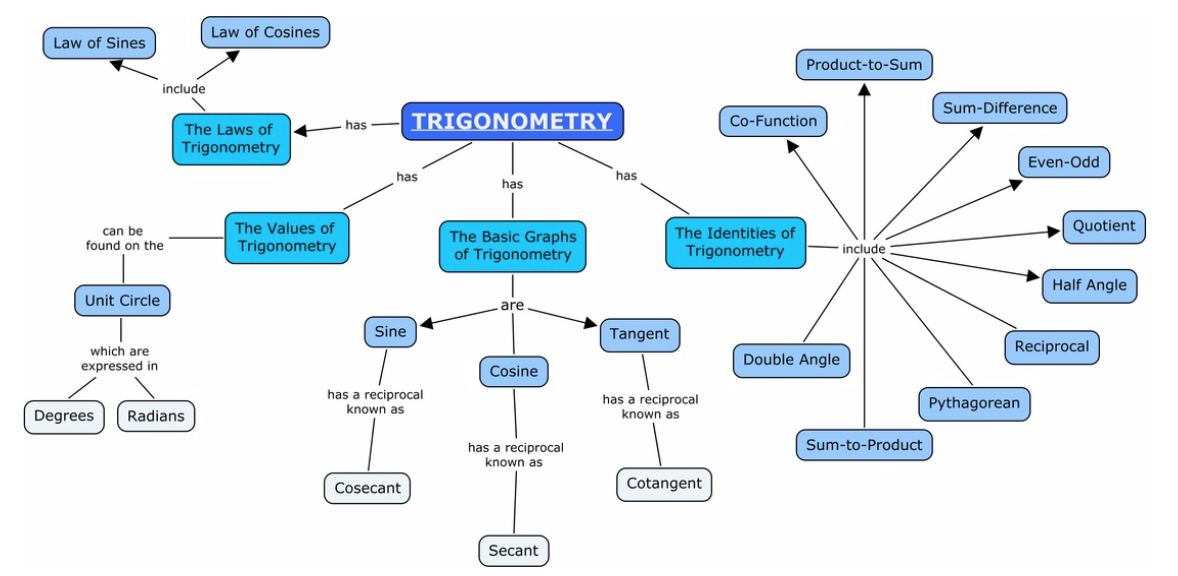
\includegraphics[width=\linewidth]{paraprofcap_mapaconceitual.png}
    \caption{Mapa conceitual da Trigonometria proposto por \citet{chigonga2016}.}
    \label{paraoprofcap_mapaconceitual}
\end{figure}
\citet{chigonga2016} também estudou dificuldades dos estudantes ao estudarem Trigonometria, em especial, ao resolverem equações trigonométricas, e menciona que os estudantes não compreendem a razão pelo o qual seno, cosseno e tangente de certos ângulos assumem valores negativos. 
%
O autor também apresenta um mapa conceitual, que pode ser visto na \Fref{paraoprofcap_mapaconceitual}, mostrando a gama de conexões dessa área. Essas conexões precisam ficar claras para os estudantes, de forma que eles percebam a Trigonometria como um todo e não como partes independentes dissociadas de significado.

\citeauthor{feijo2018} afirma que ``mesmo os alunos que apresentam entendimento sobre algum dos muitos ramos da Trigonometria (prioritariamente as razões trigonométricas) [...], o têm de forma rasa e desconexa com os demais ramos"  \citep[p. 52]{feijo2018}(2018, p. 52) . 
% 
Ela ainda constata que os erros cometidos pelos estudantes ocorrem desde o uso das definições e conceitos, até nas manipulações e generalizações.

Diante das dificuldades encontradas pelos estudantes ao estudar Trigonometria, concluímos que este ramo da Matemática requer um grande cuidado para ser apresentado aos estudantes do Ensino Médio.
%
A Trigonometria assume um papel importante dentro da Matemática por sua origem histórica e por sua aplicação em outras áreas.
%
Além disso, seu aprendizado mostra que o estudante foi capaz de articular raciocínio algébrico, geométrico e gráfico, atingindo um nível de abstração relevante em Matemática \citep{weber2005}. 

Alguns autores sugerem que ensinar Matemática, em especial Trigonometria, através de atividades pode ser um facilitador do processo de ensino e aprendizagem \citep{costa1997, mendes2001, silva2011}. 
%
Nesse contexto, consideramos atividade toda tarefa delegada aos alunos para ser trabalhada individualmente ou em grupo, em sala de aula ou fora dela, com o auxílio do professor ou não.
%
Cada atividade, ao ser realizada, levará o estudante a atingir um objetivo específico e compreender um determinado conceito.

Em seu estudo, \citeauthor{costa1997} propõe duas sequências didáticas distintas para introduzir conceitos trigonométricos. 
%
Seu objetivo é introduzir os conceitos de maneira significativa e, a partir disso, investigar como se deu a construção do conhecimento. 
%
A autora compara os resultados obtidos com o uso das sequências didáticas e afirma que certamente o conteúdo foi melhor absorvido com essas atividades do que da maneira tradicional. 
%
Já \citeauthor{mendes2001} utiliza atividades que envolvem o contexto histórico da Trigonometria como recurso metodológico.
%
O autor apresenta uma forma de repensar as aulas de Matemática conduzindo o aluno pelo caminho da descoberta e construção do conhecimento.
%
\citeauthor{silva2011} faz uso de atividades de modelagem, utilizando recursos computacionais e materiais concretos para levar o conhecimento de Trigonometria para sua sala de aula. 
%
Segundo a autora, além de contribuir para o aprendizado do aluno, a abordagem do conteúdo por meio de de atividades serviu para modificar a forma com que ela própria ensina em suas turmas, e abandonar o modelo definição, exemplo e exercício sempre utilizado em suas aulas.

%Outra possibilidade seria utilizar ferramentas computacionais para .... Falar disso? Não temos foco nisso né?

Diante da problemática mencionada e da necessidade de trabalhar com problemas em variados contextos, conforme sugerido pela BNCC, neste capítulo buscamos apresentar a Trigonometria por meio de atividades que exploram situações práticas de diversos contextos de forma dinâmica, valorizando o pensamento construtivo do estudante e evitando um foco puramente mecânico. 

%Pesquisas, como a de Blackett apontam que o uso de ferramentas computacionais pode ser muito útil no ensino/aprendizagem da trigonometria. XXXXc
%BLACKETT, Norman; TALL, David O. Gender and the versatile learning of trigonometry using computer software. Proceedings of the 15th conference of the International Group for the Psychology of Mathematics Education, 1991, 1, 144–151.

%%%%%%%%%%%%%%%%%%%%%%%%%%%%%%%%%
\section*{Objetivos Gerais}
%%%%%%%%%%%%%%%%%%%%%%%%%%%%%%%%%

De maneira geral, pretendemos levar o aluno a:

\begin{itemize}
\item reconhecer a importância de relações válidas no triângulo para resolver problemas, além das relações métricas do triângulo retângulo;
%
\item compreender as razões trigonométricas de um ângulo agudo a partir da semelhança de triângulos;
%
\item aplicar as razões trigonométricas na resolução de problemas que envolvam triângulos;
%
\item calcular o valor de seno, cosseno e tangente para ângulos com valores entre $0^\circ$ e $180^\circ$;
%
\item conhecer dois importantes resultados da Trigonometria:  Lei dos Senos e a Lei dos Cossenos;
%
\item aplicar a Lei dos Senos e a Lei dos Cossenos na resolução de problemas de diversas áreas do conhecimento.
\end{itemize}

%%%%%%%%%%%%%%%%%%%%%%%%%%%%%%%%%
\subsection*{Pré-requisitos}
%%%%%%%%%%%%%%%%%%%%%%%%%%%%%%%%%
\begin{habilities}{EF06MA19}
Identificar características dos triângulos e classificá-los em relação às medidas dos lados e dos ângulos.

\tcbsubtitle{EF06MA25} Reconhecer a abertura do ângulo como grandeza associada às figuras geométricas.

\tcbsubtitle{EF06MA26} Resolver problemas que envolvam a noção de ângulo em diferentes contextos e em situações reais, como ângulo de visão.

\tcbsubtitle{EF06MA27} Determinar medidas da abertura de ângulos, por meio de transferidor e/ou tecnologias digitais.

\tcbsubtitle{EF07MA24} Construir triângulos, usando régua e compasso, reconhecer a condição de existência do triângulo quanto à medida dos lados e verificar que a soma das medidas dos ângulos internos de um triângulo é $180^\circ$.

\tcbsubtitle{EF09MA11} Resolver problemas por meio do estabelecimento de relações entre arcos, ângulos centrais e ângulos inscritos na circunferência, fazendo uso, inclusive, de softwares de geometria dinâmica.

\tcbsubtitle{EF09MA12} Reconhecer as condições necessárias e suficientes para que dois triângulos sejam semelhantes.

\tcbsubtitle{EF09MA13} Demonstrar relações métricas do triângulo retângulo, entre elas o teorema de Pitágoras, utilizando, inclusive, a semelhança de triângulos.
\end{habilities}

%%%%%%%%%%%%%%%%%%%%%%%%%%%%%%%%%
\subsection*{Distratores}
%%%%%%%%%%%%%%%%%%%%%%%%%%%%%%%%%

A partir de nossa prática docente e das pesquisas da área, apontamos dois principais distratores ligados a este conteúdo:

\begin{itemize}
\item Os estudantes frequentemente não associam o cálculo do seno, cosseno e tangente a um ângulo. 

\item Segundo \citet{weber2005}, os estudantes demonstram dificuldade em estimar seno de ângulos não notáveis, por exemplo, $\sen(20^\circ)$.

\item Segundo \citet{feijo2018}, os estudantes costumam confundir o valor de seno e cosseno de um ângulo.

\item Segundo \citet{silvaneto2006}, os estudantes costumam ter problemas para encontrar, em um triângulo, o lado oposto ou adjacente de um ângulo específico.
\end{itemize}
\end{apresentacao}


\def\currentcolor{session1}
\begin{texto}
{
    \section{Seção 1: Trigonometria no triângulo retângulo}

    Nesta seção são apresentados os fundamentos da Trigonometria. Inicialmente, apresentamos um breve histórico de suas origens, ressaltando a ideia do surgimento da Trigonometria através das necessidades e curiosidades dos nossos antepassados em medir distâncias, comprimentos e ângulos. Depois disso, introduzimos os conceitos básicos da Trigonometria e destacamos algumas situações reais onde podemos utilizá-la. 

    O estudo da Trigonometria está intimamente relacionado com alguns conceitos da Geometria Euclidiana tais como ângulos, semelhança, arcos da circunferência, entre outros. Diante dessa realidade, procuramos levar o aluno a rever alguns desses conceitos nas partes introdutórias desta seção.

    Nesta primeira seção, são introduzidas as razões trigonométricas de ângulos agudos: seno, cosseno e tangente. Também estabelecemos as principais relações e propriedades dessas razões trigonométricas, destacando os seus valores para alguns ângulos específicos, os chamados ângulos notáveis. Tentamos também destacar que os ângulos notáveis raramente aparecem em problemas que surgem na prática. 

    Ao longo do texto, por diversas vezes, o aluno é convidado a fazer as suas próprias reflexões, questionamentos e sugerir respostas para suas perguntas, fazendo-o pensar sobre os conceitos desenvolvidos na seção e como utilizá-los para modelar e resolver problemas que fazem parte do seu cotidiano. Além disso, o texto apresenta atividades que têm por objetivo desenvolver, fixar e mostrar o alcance dos conceitos desenvolvidos nesta seção.

    No decorrer desta seção, será necessário calcular seno, cosseno e tangente de ângulos não notáveis. Para isso, sugerimos utilizar a tabela trigonométrica disponibilizada no final do capítulo. Caso seja possível utilizar meios eletrônicos para os cálculos que envolvem ângulos não notáveis, o professor também pode optar por eles.
}
\end{texto}
\clearmargin
\clearmargin
\begin{objectives}{Alguns quocientes constantes a partir de um ângulo dado}
{
\begin{itemize}
\item Resgatar ideias da Geometria que serão úteis para  desenvolver o conteúdo deste capítulo, como ângulos, triângulos, semelhança de triângulos e etc; relembrar a proporcionalidade existente entre lados de triângulos semelhantes.

\item \textbf{Conceitos abordados}: triângulos retângulos e semelhança de triângulos.
\end{itemize}
}{1}{1}
\end{objectives}
\begin{sugestions}{Alguns quocientes constantes a partir de um ângulo dado}
{
Sugerimos ao professor uma revisão do capítulo {\textit{Semelhança de Triângulos}} antes de utilizar esta atividade em sala de aula. A semelhança de triângulos será primordial para resolver os itens (d) e (e) desta atividade. No item (d), sugerimos ao professor que medie uma discussão entre os estudantes que o leve a perceber a semelhança existente entre os triângulos trabalhados. Já no item (e), é preciso levar o estudante a justificar as igualdades fornecidas no enunciado sem fazer nenhum cálculo e sim usando semelhança de triângulos. 

\textbf{Organização da turma}: individual
}{1}{1}
\end{sugestions}
\begin{answer}{Alguns quocientes constantes a partir de um ângulo dado}
{
\begin{enumerate}
\item Usando o segmento $PQ$ como unidade de comprimento obtemos as seguintes medidas:

\begin{table}[H]
\centering
\begin{tabular}{|c|c|c|c|c|c|}
\hline
$\tmat{AB}$   & $\tmat{AG}$ & $\tmat{AF}$ & $\tmat{BC}$ & $\tmat{GE}$ & $\tmat{FD}$   \\  \hline
$16$ u.c.  & $9$ u.c. & $4$ u.c.  &  $12$ u.c. &  $6,8$ u.c. & $3$ u.c.   \\\hline
\end{tabular}
\caption{Medidas dos triângulos da \Fref{Proporcao1}.}
\end{table}
\end{enumerate}
}{1}
\end{answer}
\clearmargin
\mspace{.25em}
\begin{answer}{Alguns quocientes constantes a partir de um ângulo dado}
{
\begin{enumerate}\setcounter{enumi}{1}
\item A partir dos valores da tabela anterior, segue que:
   
\begin{table}[H]
\centering
\begin{tabular}{|c|e{1.5cm}|e{1.5cm}|e{1.5cm}|} 
\hline
\tcolor{} & $\dfrac{BC}{AB}$    & $\dfrac{GE}{AG}$ & $\dfrac{FD}{AF}$  \tabularnewline 
 \hline
\tcolor{Quociente} & $\dfrac{12}{16}$   & $\dfrac{6,8}{9}$  & $\dfrac{3}{4}$ \tabularnewline
\hline 
\tcolor{Aproximação} & $0{,}75$ & $0{,}755$ & $0{,}75$   \tabularnewline
\hline 
\end{tabular}
\caption{Quocientes e aproximações obtidos a partir dos dados da  \Fref{Proporcao1}.}
\label{Table_quocientes2}
\end{table}

\item{}
Os quocientes $\frac{BC}{AB}, \frac{GE}{AG}$ e $\frac{FD}{AF}$ são aproximadamente iguais.

\item{}
Note que, $C\hat{A}B=E\hat{A}G=D\hat{A}F$ e $A\hat{B}C=A\hat{G}E=A\hat{F}D$. Sendo assim, os triângulos $ABC, AGE$ e $AFD$ possuem ângulos internos congruentes, o que implica que eles são semelhantes e, consequentemente, seus lados correspondentes são proporcionais. Daí, com base no que foi aprendido no capítulo \textit{Semelhança de Triângulos} vale que:
$$\frac{BC}{AB}=\frac{GE}{AG}=\frac{FD}{AF}.$$

Sendo assim, as aproximações encontradas na segunda linha da \Tref{Table_quocientes2} são, na verdade, iguais e não aproximadamente iguais. A pequena variação de valores encontrada é fruto da estimativa da medida do segmento $GE$ como sendo $6,8$u.c.

\item{}
Como foi mencionado no item anterior, os triângulos $ABC, AGE$ e $AFD$ são semelhantes (pois apresentam ângulos correspondentes congruentes). Sendo assim, vale que: 
$$\dfrac{AB}{AC}=\dfrac{AG}{AE}=\dfrac{AF}{AD}.$$
$$\dfrac{BC}{AC}=\dfrac{GE}{AE}=\dfrac{FD}{AD}.$$
\end{enumerate}
}{1}
\end{answer}
\begin{objectives}{Acessibilidade}
{
\begin{itemize}
\item Comparar triângulos em uma situação real
\item \textbf{Conceitos abordados}: triângulos retângulos, semelhança de triângulos e inclinação.
\end{itemize}
}{1}{2}
\end{objectives}
\clearmargin
\begin{sugestions}{Acessibilidade}
{
Nesta atividade será definida a inclinação de uma rampa de acessibilidade e o aluno será convidado a calcular a inclinação de duas rampas. Essas duas rampas possuem medidas diferentes, mas a mesma inclinação. Este fato está ligado à semelhança de triângulos e será ser explorado no item \titem{c)} da atividade. Essa será mais uma oportunidade do aluno trabalhar em uma situação real envolvendo triângulos semelhantes.

\textbf{Organização da turma}: individual.

\textbf{Enriquecimento da discussão}: essa atividade tem como objetivo reiterar ao estudante que, ao observarmos o mundo ao nosso redor, a Matemática está sempre presente. Nesta atividade, o estudante é convidado a pensar em um problema real, onde ele poderá aplicar estratégias simples para solucioná-lo. Além disso, essa atividade revela ao aluno que nos problemas da vida real não há questionamentos prontos do tipo ``faça'', ``determine'' ou ``calcule''. Na verdade, é ele quem deve tomar a decisão sobre o que calcular ou determinar para responder a certos questionamentos.
}{1}{1}
\end{sugestions}
\clearmargin
\begin{answer}{Acessibilidade}
{
\begin{enumerate}


\item{}
Segundo a \Fref{Cadeirante}, o primeiro trecho da rampa possui altura de $30\text{cm}=0,30$m e comprimento horizontal de $3,60$m. Então, a inclinação desta rampa é 
$$\frac{0{,}30}{3{,}60}\cdot 100\approx 8{,}33\%.$$

Já o segundo trecho da rampa possui altura de $80-30=50\text{cm}=0,5$m e comprimento de $6$m. Logo, sua inclinação é dada por 
$$\frac{0{,}50}{6}\cdot 100\approx 8{,}33\%.$$

Sendo assim, o dois trechos da rampa estão de acordo com a norma NBR9050 da ABNT já que possuem inclinação acima de $5\%$.

\item{}
A vista lateral das duas rampas está representada na  \Fref{Rampadef} pelos triângulos retângulos $ABC$ (primeiro trecho) e $DEF$ (segundo trecho).
\begin{figure}[H]
    \centering
    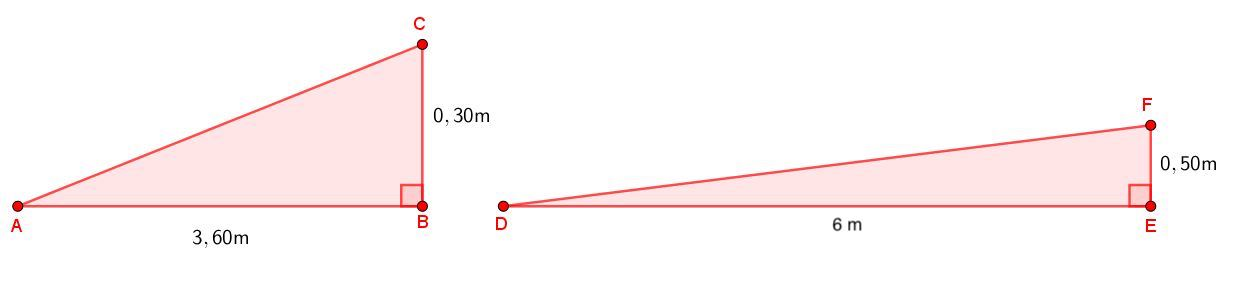
\includegraphics[scale=0.275]{Rampadef.JPG}
    \caption{Vista lateral das rampas de acessibilidade da  \Fref{Cadeirante}.}
    \label{Rampadef}
\end{figure}

\item{}
Note que 
$$\fra{BC}{AB}=\fra{EF}{DE},$$
e por isso, ao fazer os cálculos da inclinação das rampas encontramos o mesmo valor para os dois trechos. 
Logo, os ângulos $A\hat{B}C$ e $D\hat{E}F$ dos triângulos $ABC$ e $DEF$, respectivamente, são congruentes e $\fra{BC}{AB}=\fra{EF}{DE}$, então os triângulos $ABC$ e $DEF$ são semelhantes.

Isto nos leva a concluir que duas rampas possuem a mesma inclinação, se e só semente se, suas vistas laterais são triângulos retângulos semelhantes. 
\end{enumerate}
}{1}
\end{answer}

\explore{Trigonometria, uma Necessidade Humana?}

A Trigonometria lida com as relações entre as medidas dos ângulos e dos lados de um triângulo. O seu surgimento está ligado, possivelmente, à necessidade de nossos antepassados em medir distâncias inacessíveis, como a altura de uma montanha, de um monumento ou do raio terrestre. Esse estudo remonta aos primórdios da história da Mesopotâmia e do Egito, mas alcançou novo patamar a partir do filósofo e matemático grego Tales de Mileto, que viveu no século V a.C. e foi a primeira pessoa na história a quem se atribuem descobertas matemáticas.

Na sociedade moderna, o uso da Trigonometria extrapolou as suas motivações iniciais e passou a fazer parte, por exemplo, dos sistemas modernos de navegação utilizados por aviões e embarcações. Pode não parecer, mas a Trigonometria está muito presente em nossa vida nos dias atuais. Ela está em nossas mãos quando utilizamos um telefone celular para nos guiar para um dado endereço, ou precisamos de uma previsão do valor que pagaremos por uma viagem com um motorista de aplicativo ou mesmo quando jogamos um jogo eletrônico. 

A Trigonometria está espalhada por toda parte! Muitas vezes ela não está tão explícita como outros conceitos matemáticos tais como percentagens, proporcionalidade, áreas e volumes. Porém, com um olhar mais cuidadoso e conhecimento básico dessa teoria, podemos identificá-la em diversas ocasiões e situações do mundo moderno, e em diversas áreas como Engenharia, Arquitetura e Ciências Naturais.

Uma das primeiras aplicações da Trigonometria foi a determinação da medida do raio do planeta Terra feita pelo famoso sábio grego Eratóstenes, conhecido como o ``pai da Geografia''. Eratóstenes, com uma impressionante precisão, apontou que o raio da Terra mede $6.370$ km, como veremos adiante. Ele nasceu em Cirene, na Líbia, em 276 a.C. e passou a maior parte da sua vida em Alexandria, no Egito, tendo sido diretor da sua famosa biblioteca. 

\begin{figure}[H]
    \centering
    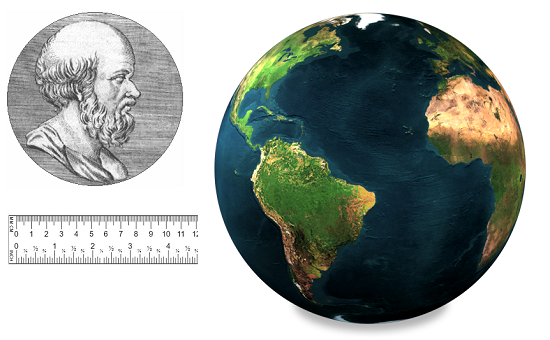
\includegraphics[width=.55\linewidth]{Eratostenes.png}
    \caption{Eratóstenes. Fonte: https://bit.ly/3iK6cIW}
    \label{Eratostenes}
\end{figure}

Para obter uma aproximação da medida do raio da Terra, Eratóstenes observou e utilizou os seguintes fatos:
\begin{itemize}
    \item{}
    no primeiro dia de verão na cidade de Siena (atual cidade de Assuã no Egito), o Sol ao meio-dia está na vertical;
    
    \item{}
    no mesmo dia e à mesma hora, na cidade de Alexandria, o ângulo entre uma vara colocada na vertical e a linha que une a extremidade de cima à ponta da sombra é de $\frac{1}{50}$  de uma volta completa, ou seja, $\dfrac{1}{50} \cdot 360^\circ=7,2^\circ$;
    
    \item{}
    Siena fica exatamente ao Sul de Alexandria;
    
    \item{}
    a distância entre as duas cidades é de cerca de $800$km;
    
    \item{}
    os raios luminosos provenientes do Sol são linhas paralelas;
    
    \item{}
    a amplitude do ângulo  Siena—Centro da Terra—Alexandria é igual à do ângulo que os raios de Sol em Alexandria fazem com a vertical.
\end{itemize}

Essas informações estão resumidas na  \Fref{Eratostenes2}:

\begin{figure}[H]
    \centering
    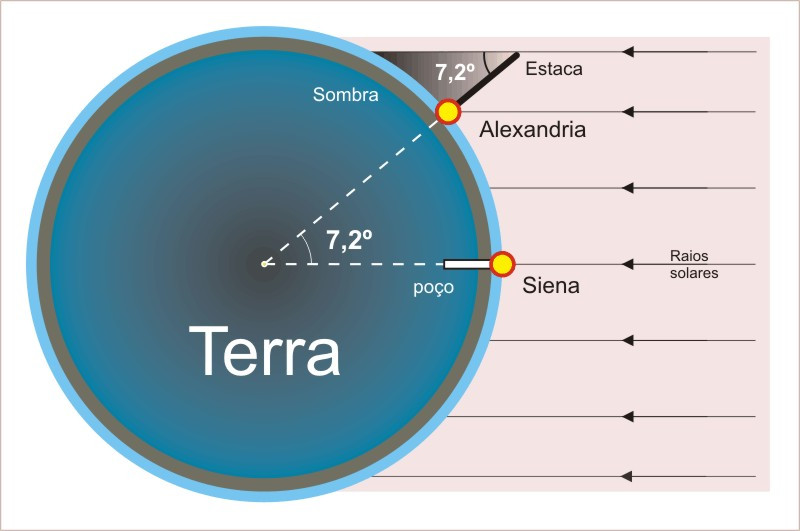
\includegraphics[width=.7\linewidth]{Eratostenes2.jpg}
    \caption{Medindo o raio terrestre. Fonte: https://bit.ly/33a6uEN}
    \label{Eratostenes2}
\end{figure}

 A partir dessas informações, Eratóstenes obteve uma estimativa para a medida do raio terrestre, utilizando uma simples proporção: o ângulo central de medida $7,2^\circ$ corresponde a um arco de comprimento $800$km sobre a superfície terrestre, enquanto que o ângulo central de $360^\circ$ corresponde ao comprimento de uma circunferência que circunda superfície terrestre. Supondo que a medida do raio da Terra (supostamente esférica) seja $R$, o comprimento dessa circunferência é $2\pi R$, onde $\pi \approx 3,14$. Assim,
 $$\frac{800}{7,2^\circ}=\frac{2\pi R}{360^\circ} \iff R \approx \frac{360^\circ \cdot 800}{7,2^\circ \cdot 2 \cdot 3,14}  \iff R\approx 6.370 \text{km}.$$

 O valor aceito atualmente para o raio terrestre é $6.371$km, portanto, o erro cometido por Eratóstenes foi de aproximadamente $1$km, que percentualmente corresponde a $\frac{1}{631} \approx 0,01\%$. Esta estimativa é surpreendente, diante dos poucos recursos disponíveis na época. 
 
 O vídeo disponível no endereço \url{https://www.youtube.com/watch?v=BjO9G4XGpiE} ilustra a determinação da medida do raio da Terra por Eratóstenes.

\newpage
\begin{task}{Alguns quocientes constantes a partir de um ângulo dado}

Diferentemente de outros ramos da Matemática, a Trigonometria muitas vezes não aparece de forma explícita ao nosso redor, mas se pararmos para observar com mais atenção podemos identificar diversas situações onde ela está presente. Por exemplo, a  \Fref{Rampas} mostra uma rampa bastante utilizada nas oficinas de manutenção de automóveis, que é formada por diversos triângulos retângulos.
\begin{figure}[H]
    \centering
    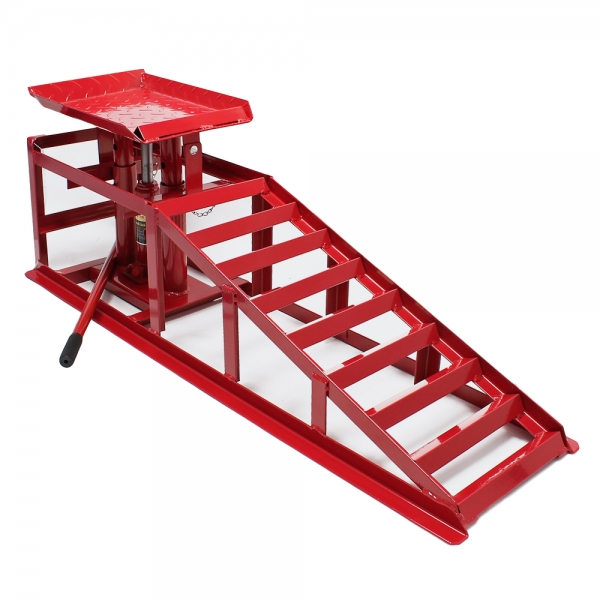
\includegraphics[scale=0.2]{Rampa1.jpg}
    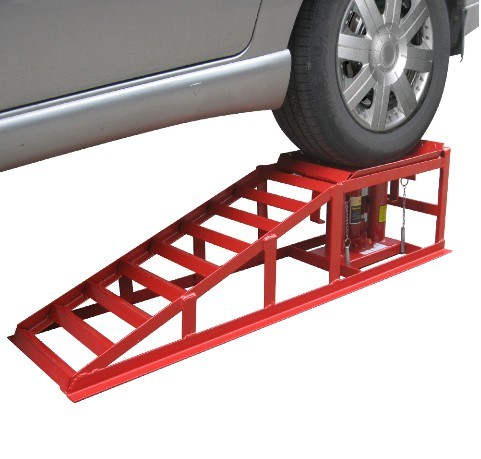
\includegraphics[scale=0.4]{Rampa2.jpg}
    \caption{Rampa para manutenção de automóveis. Fonte: https://bit.ly/32oQgWe}
    \label{Rampas}
\end{figure}
%Falta fonte:https://www.google.com/search?q=lava+jato+rampa&tbm=isch&ved=2ahUKEwiQ0eLU3ODqAhWMBbkGHUi0CdkQ2-cCegQIABAA&oq=lava+jato+rampa&gs_lcp=CgNpbWcQA1CLF1jGH2DdIWgAcAB4AIABhAKIAcwHkgEFMC41LjGYAQCgAQGqAQtnd3Mtd2l6LWltZ8ABAQ&sclient=img&ei=tR4YX9CiLYyL5OUPyOimyA0&bih=937&biw=1920&rlz=1C1SQJL_enBR900BR900#imgrc=vXMxb4NmykjEMM&imgdii=Piq8vyiR1wN8BM

\begin{enumerate}
    \item{}
    A  \Fref{Proporcao1} representa a vista lateral de parte da rampa, onde identificamos os triângulos retângulos $ABC, AGE$ e $AFD$, desenhada sobre uma malha quadriculada.
    \begin{figure}[H]
    \centering
    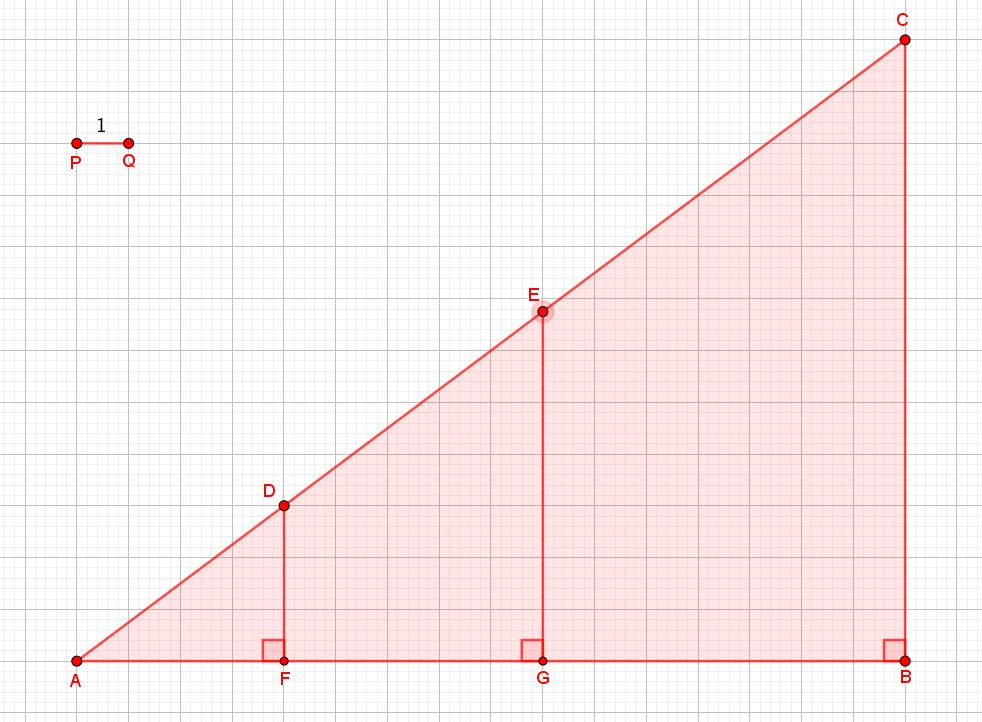
\includegraphics[scale=0.3]{Proporcao1.JPG}
    \caption{Triângulos retângulos na lateral da rampa.}
    \label{Proporcao1}
\end{figure}

Utilizaremos o segmento $PQ$ como uma unidade de comprimento (u.c.), isto é, $PQ=1$ u.c. Com base na  \Fref{Proporcao1} e utilizando a unidade de comprimento mencionada, obtenha estimativas para os comprimentos dos segmentos indicados na  \Tref{Table_ladostriangulos}.

\begin{table}[H]
\centering
\begin{tabular}{|c|c|c|c|c|c|}
\hline
 $\tmat{AB}$    & $\tmat{AG}$ & $\tmat{AF}$ & $\tmat{BC}$ & $\tmat{GE}$ & $\tmat{FD}$   \\  \hline
     &  &   &   &   &    \\\hline
\end{tabular}
\caption{Medidas dos triângulos da  \Fref{Proporcao1}.}
\label{Table_ladostriangulos}
\end{table}

\item{}
A partir das estimativas obtidas no item anterior, indique na \Tref{Table_quocientes} os quocientes pedidos e calcule suas aproximações. Caso seja necessário, utilize $3$ casas decimais para calcular as aproximações pedidas.

\begin{table}[H]

\centering
\begin{tabular}{|c|e{1.5cm}|e{1.5cm}|e{1.5cm}|} 
\hline
\tcolor{}& $\dfrac{BC}{AB}$    & $\dfrac{GE}{AG}$ & $\dfrac{FD}{AF}$    \tabularnewline  \hline
\tcolor{Quociente} &  &  & \tabularnewline \hline 
\tcolor{Aproximação} &  &  & \tabularnewline \hline 
\end{tabular}
\caption{Quocientes e aproximações obtidos a partir dos dados da \Fref{Proporcao1}.}
\label{Table_quocientes}
\end{table}


\item{}
Analisando a \Tref{Table_quocientes}, o que você percebe?

\item{}
Analise novamente os triângulos da \Fref{Proporcao1} e verifique se há alguma relação entre eles. E agora, você mantém sua resposta ao item anterior?

\item{} Justifique as igualdades a seguir:
$$\dfrac{AB}{AC}=\dfrac{AG}{AE}=\dfrac{AF}{AD},$$
$$\dfrac{BC}{AC}=\dfrac{GE}{AE}=\dfrac{FD}{AD}.$$

\end{enumerate}
\end{task}

\begin{task}{Acessibilidade}
Segundo o Estatuto da Pessoa com Deficiência, cujo objetivo principal é assegurar e promover condições de igualdade a todas as pessoas, todo indivíduo que possui alguma deficiência tem direito à igualdade de oportunidades. 

\begin{figure}[H]
    \centering
    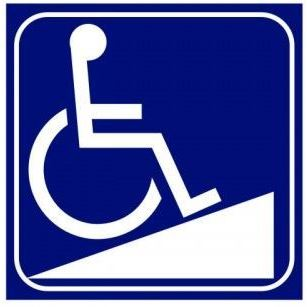
\includegraphics[scale=0.6]{Cadeirante2.JPG}
    \caption{Símbolo universal de acessibilidade. Fonte: \url{https://bit.ly/3lbX3ey}.}
    \label{Cadeirante2}
\end{figure}
%https://assimcomovoce.blogfolha.uol.com.br/2012/05/28/calcadas-para-cadeirantes/


Em termos de acessibilidade, todas as edificações públicas e privadas que se destinam a uso coletivo devem, por lei, ser adaptados à pessoa com deficiência. Para isso, dentre muitas outras coisas, as edificações devem conter as chamadas rampas de acessibilidade. 

Uma rampa de acessibilidade é uma adaptação realizada nas construções que facilita a livre movimentação de cadeirantes e pessoas com mobilidade reduzida, que normalmente não podem fazer uso de escadas. A inclinação de uma rampa é a relação entre sua altura $h$ e seu comprimento horizontal $c$ expressa em porcentagem, ou seja, a inclinação em porcentagem $i$ da rampa é dada por 
$$i=\frac{h}{c}\cdot 100.$$
A \Fref{Rampapercentual} mostra a vista lateral de algumas rampas e suas inclinações. Na primeira delas, por exemplo, a rampa possui altura $1$ e comprimento $20$. Neste caso, a inclinação da rampa é de $5\%$.

\begin{figure}[H]
    \centering
    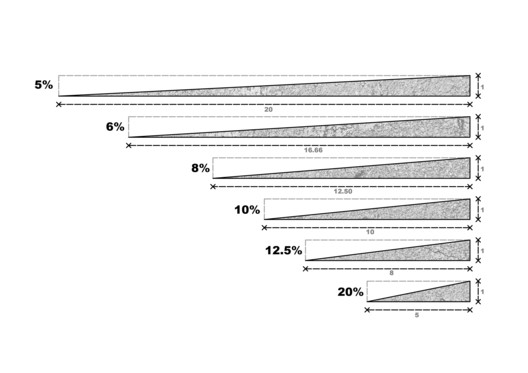
\includegraphics[scale=3]{Rampapercentual.jpg}
    \caption{Inclinação percentual de uma rampa. Fonte:https://bit.ly/3lbX3ey.}
    \label{Rampapercentual}
\end{figure}



Segundo a norma NBR 9050 da Associação Brasileira de Normas Técnicas (ABNT), para ser considerada uma rampa, sua inclinação deve ser igual ou superior a $5\%$. 

A \Fref{Cadeirante} ilustra  o acesso a um prédio comercial que foi adaptado para pessoas com dificuldade de locomoção. Esse sistema de acessibilidade é constituído por duas rampas com as dimensões fornecidas na figura.

\begin{figure}[H]
    \centering
    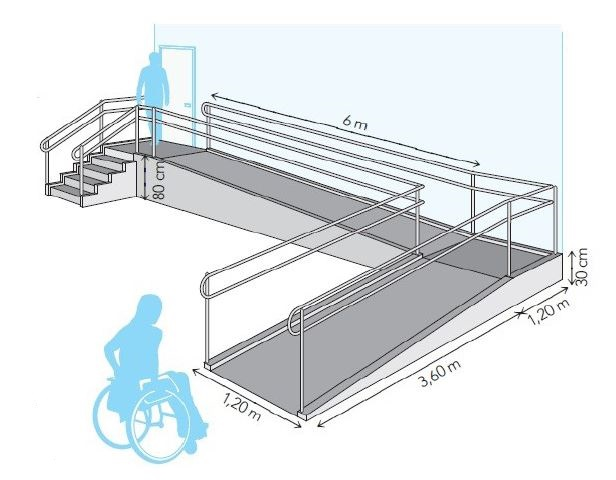
\includegraphics[scale=0.7]{Cadeirante.JPG}
    \caption{Rampas de acessibilidade de um prédio comercial. Fonte: https://bit.ly/3guY3XA.}
    \label{Cadeirante}
\end{figure}
%https://www.google.com/search?q=rampa+de+acesso+a+cadeirantes&tbm=isch&ved=2ahUKEwis2bO4i6brAhVRDdQKHR0KB8IQ2-cCegQIABAA&oq=rampa+de+acesso+a+cadeirantes&gs_lcp=CgNpbWcQAzoICAAQBxAFEB5Qz-8DWN2BBGCNhgRoAHAAeACAAdMBiAH4DJIBBTAuNi4zmAEAoAEBqgELZ3dzLXdpei1pbWfAAQE&sclient=img&ei=yHw8X6zVKNGa0AadlJyQDA&bih=888&biw=1920#imgrc=wCGGhfoYIGad2M&imgdii=LnuW4GPLMbnr6M


\begin{enumerate}
\item{}
Calcule a inclinação das duas rampas da \Fref{Cadeirante} e verifique se elas atendem à norma NBR 9050. Caso seja necessário fazer aproximações, utilize duas casas decimais.

\item{}
Faça um desenho que represente a vista lateral de cada uma das rampas da \Fref{Cadeirante}. 

\item{}  
Analisando os dois desenhos feitos no item anterior, é possível encontrar alguma relação entre eles que justifique os valores das inclinações encontrados no item \titem{a)}.
\end{enumerate}

\end{task}

\arrange{As principais razões trigonométricas}

Por meio dos quocientes trabalhados nas atividades anteriores, vamos introduzir algumas razões trigonométricas associadas a um ângulo agudo dado. Essas razões são ferramentas matemáticas simples, mas extremamente úteis para tratar problemas reais, como por exemplo, determinar distâncias que não podem ser medidas diretamente. 

Vamos primeiramente fixar um ângulo agudo $P\hat{O}Q$ de medida $\alpha$. Sobre o lado $OP$ de $P\hat{O}Q$, considere dois pontos quaisquer $A_1$ e $A_2$ e sobre o lado $OQ$, os pontos $B_1$ e $B_2$ de modo que os triângulos $A_1B_1O$ e $A_2B_2O$ sejam retângulos em $B_1$ e $B_2$, respectivamente, como na \Fref{TriagRet1}.

\begin{figure}[H]
    \centering
    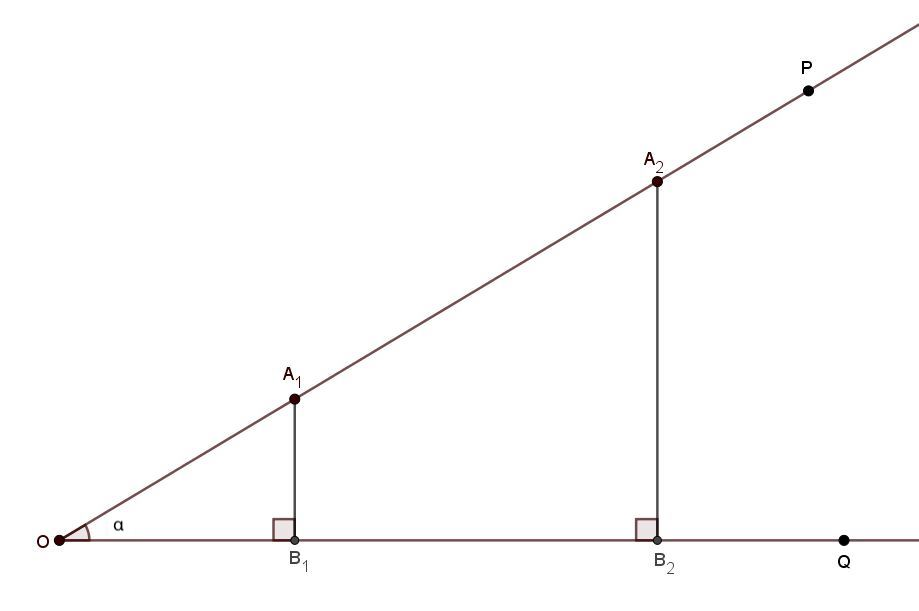
\includegraphics[scale=0.35]{TriagRetSem1.JPG}
    \caption{Triângulos retângulos construídos a partir do ângulo $\alpha$.}
    \label{TriagRet1}
\end{figure}

Os triângulos $A_1B_1O$ e  $A_2B_2O$ são semelhantes (por que?), então
\begin{equation}
\frac{A_1B_1}{A_2B_2}=\frac{OB_1}{OB_2}=\frac{OA_1}{OA_2}=k \label{sec1_razaodesem}
\end{equation}
onde $k$ é razão de semelhança entre $A_1B_1O$ e $A_2B_2O$.

Neste caso, temos
\begin{eqnarray}
A_1B_1 & = & k \cdot A_2B_2, \label{sec1_razaodesem_ig1}\\ 
OB_1 & = & k \cdot OB_2,         \label{sec1_razaodesem_ig2} \\
OA_1 & = & k \cdot O A_2.         \label{sec1_razaodesem_ig3}
\end{eqnarray}
De \eqref{sec1_razaodesem_ig1} e \eqref{sec1_razaodesem_ig3} obtemos:
\begin{equation}
\fra{A_1B_1}{OA_1}=\fra{k\cdot A_2B_2}{k \cdot OA_2}=\fra{A_2B_2}{OA_2}. \label{sec1_razaodesem_ig4}
\end{equation}
Dessa forma, a igualdade $\fra{A_1B_1}{OA_1}=\fra{A_2B_2}{OA_2}$ independe da razão de semelhança $k$. 

Neste caso, o que podemos concluir é que independentemente dos triângulos semelhantes escolhidos, a relação \eqref{sec1_razaodesem_ig4} é sempre válida. Isto significa que os quocientes $\fra{A_1B_1}{OA_1}$ e $\fra{A_2B_2}{OA_2}$ são constantes. Na verdade, esses quocientes só serão alterados se for mudada a amplitude do ângulo $\alpha$, ou seja, os quocientes $\fra{A_1B_1}{OA_1}$ e $\fra{A_2B_2}{OA_2}$ dependem apenas do ângulo $\alpha$.

Analogamente, de \eqref{sec1_razaodesem_ig1}, \eqref{sec1_razaodesem_ig2} e \eqref{sec1_razaodesem_ig3}, encontramos
\begin{eqnarray}
\fra{OB_1}{OA_1} & = \fra{k\cdot OB_2}{k \cdot OA_2} & =  \fra{OB_2}{OA_2}, \nonumber\\ 
\fra{A_1B_1}{OA_1} & =\fra{k\cdot A_2B_2}{k \cdot OB_2} & =  \fra{A_2B_2}{OB_2}. \nonumber 
\end{eqnarray}
Daí,
\begin{eqnarray}
\fra{OB_1}{OA_1} = \fra{OB_2}{OA_2}, \label{sec1_razaodesem_ig7}\\ 
\fra{A_1B_1}{OA_1} = \fra{A_2B_2}{OB_2}.  \label{sec1_razaodesem_ig8} 
\end{eqnarray}
não dependem da razão de semelhança $k$. Assim, os quocientes que compõem as relação \eqref{sec1_razaodesem_ig7} e \eqref{sec1_razaodesem_ig8} são também constantes e só dependem do ângulo $\alpha$.
    
Diante disso, cada um dos quocientes \eqref{sec1_razaodesem_ig4}, \eqref{sec1_razaodesem_ig7} e \eqref{sec1_razaodesem_ig8} recebe um nome especial e todos eles compõem o que chamamos de {\textbf{razões trigonométricas  do ângulo $\alpha$}}, visto que esses quocientes dependem exclusivamente do ângulo $\alpha$. O primeiro chamamos de seno do ângulo $\alpha$, o segundo de cosseno do ângulo $\alpha$ e o terceiro de tangente do ângulo $\alpha$. 
    
Para fixar melhor essas ideias e algumas notações, vamos considerar um triângulo  $ABC$ retângulo em $A$, construído a partir de um ângulo agudo $\alpha$, como da \Fref{TriagRet6}.     
\begin{figure}[H]
\centering
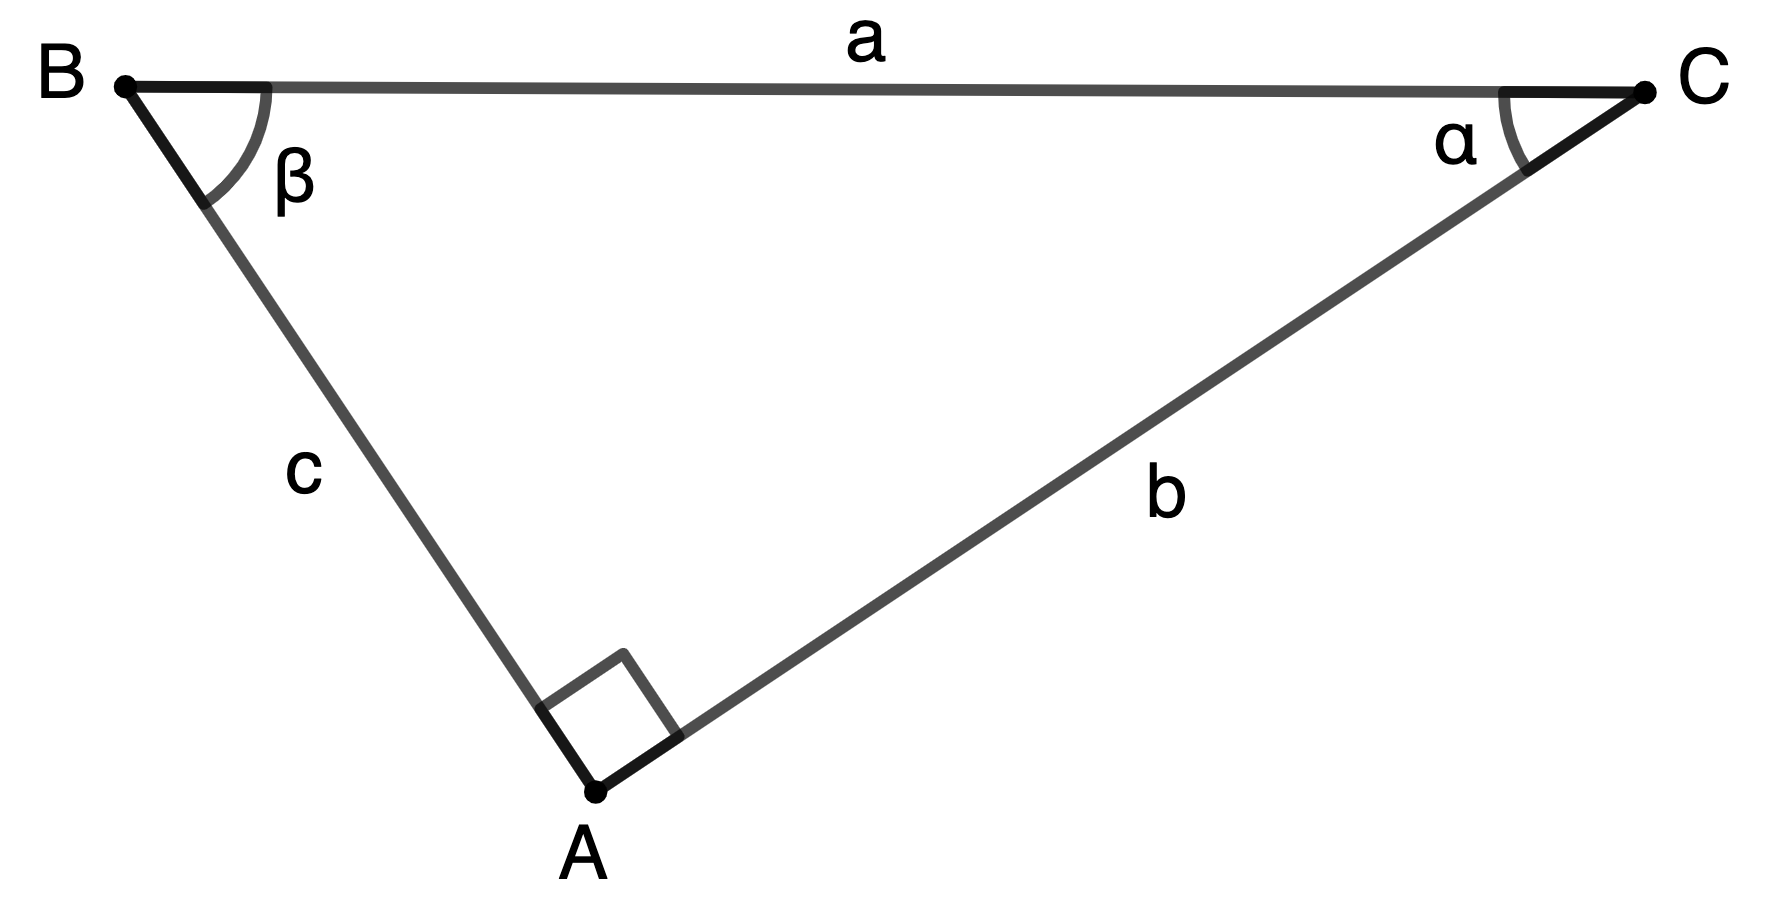
\includegraphics[scale=0.9]{sec1_triagretangulo.png}
\caption{Triângulo retângulo construído a partir de um ângulo $\alpha$ dado.}
\label{TriagRet6}
\end{figure}

As razões trigonométricas do ângulo $\alpha$ são seno de $\alpha$, cosseno de $\alpha$ e tangente de $\alpha$, e serão denotadas por $\sen\alpha, \cos \alpha$ e $\tg\alpha$, respectivamente. Usando o triângulo $ABC$, calculamos as razões trigonométricas de $\alpha$ da seguinte forma:
$$\sen\alpha=\fra{AB}{BC}=\fra{c}{a}\;,\quad\cos\alpha=\fra{AC}{BC}=\fra{b}{a} \quad\text{ e }\;\; \tg\alpha=\fra{AB}{AC}=\fra{c}{b}.$$

\begin{observationtitle}{Atenção!}
As definições de seno, cosseno e tangente de um ângulo, apesar de construídas a partir de um triângulo retângulo, independem do triângulo escolhido, como discutido anteriormente. Por isso, calculamos o seno, cosseno e tangente do ângulo $\alpha$ e não do triângulo $ABC$.
\end{observationtitle}

Note que, como o seno e o cosseno de um ângulo agudo $\alpha$ de $ABC$ são obtidos por quocientes entre as medidas de um cateto e da hipotenusa, sempre maior que o cateto, segue que os seus valores são positivos e menores que $1$. Ou seja, 
$$0 < \sen\alpha < 1 \ \ \text{e}  \ \ 0  < \cos\alpha < 1.$$

\begin{observationtitle}{Relação Fundamental}
A partir das definições dadas anteriormente, podemos encontrar outras relações importantes envolvendo o seno, cosseno e tangente de um ângulo agudo. Usando a notação da \Fref{TriagRet6} e o triângulo retângulo $ABC$, podemos observar que
$$\tg\alpha=\fra{AB}{AC}=\fra{c}{b}=\fra{\sen\alpha}{\cos\alpha}.$$

E ainda,
\begin{equation}\label{sec1_relfundamental1}
\sen^2\alpha+\cos^2\alpha=\left(\frac{c}{a}\right)^2+\left(\frac{b}{a}\right)^2=\frac{b^2+c^2}{a^2}
\end{equation}
Como $ABC$ é um triângulo retângulo, pelo teorema de Pitágoras sabemos que $a^2=b^2+c^2$. Logo, a equação \eqref{sec1_relfundamental1} pode ser reescrita da seguinte forma:
\begin{equation}\label{sec1_relfundamental2}
\sen^2\alpha+\cos^2\alpha=1.
\end{equation}

A relação \eqref{sec1_relfundamental2} é chamada de {\textbf{relação fundamental da Trigonometria}}.
\end{observationtitle}

Analisando um pouco mais o triângulo $ABC$, podemos obter as seguintes relações entre as razões trigonométricas do ângulos complementares $\alpha$ e $\beta$:
$$\sen\alpha=\cos\beta=\frac{c}{a}, \quad  \sen\beta=\cos\alpha=\frac{b}{a} \quad \text{e} \quad \tg\alpha=\fra{\sen\alpha}{\cos\alpha}=\frac{\cos\beta}{\sen\beta}=\frac{1}{\tg\beta}.$$
    
\begin{observationtitle}{Observação}
        $\bullet$ De acordo com as definições de seno e cosseno de um ângulo agudo $\alpha$, podemos concluir que num triângulo retângulo construído a partir de $\alpha$ cuja hipotenusa tem medida $a$, os seus catetos medem $a\cdot\cos\alpha$  e $a\cdot\sen\alpha$. Veja a \Fref{TriagRet3}.
    
    \begin{figure}[H]
    \centering
    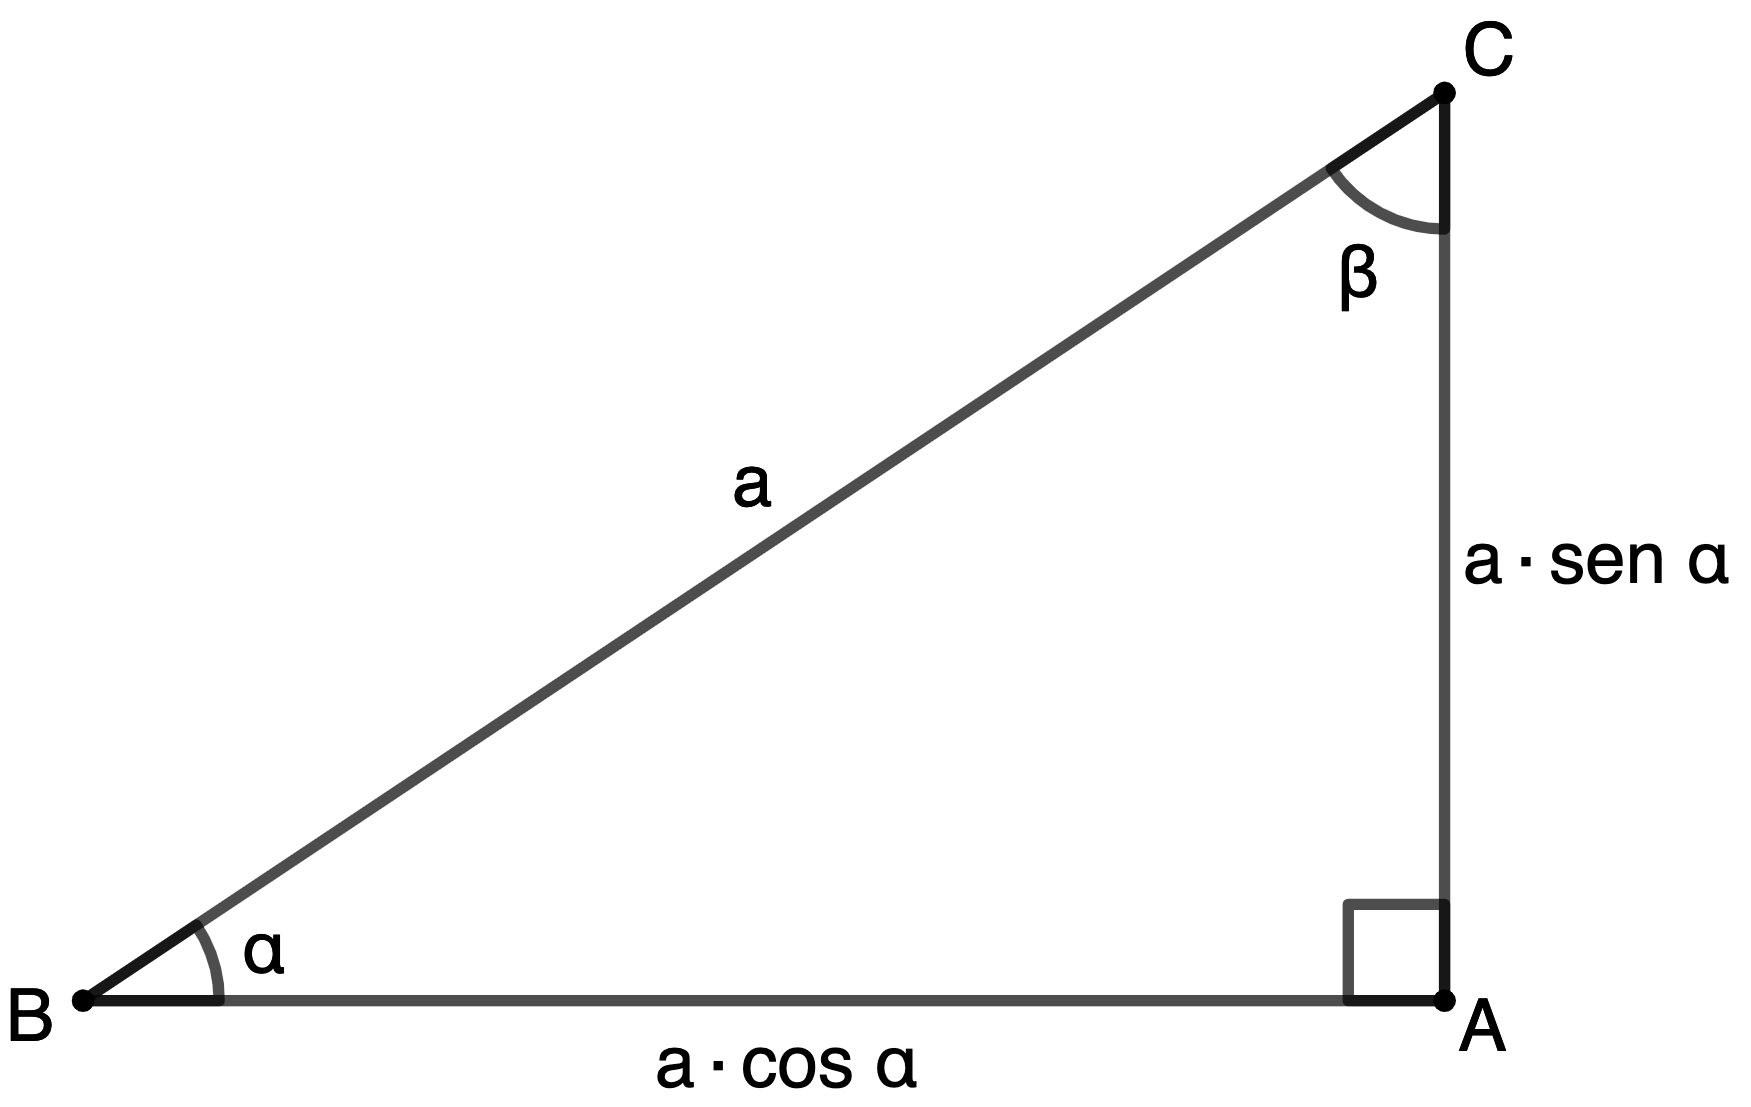
\includegraphics[scale=1]{sec1_triangret_hipa.png}
    \caption{Catetos de um triângulo retângulo com hipotenusa medindo $a$.}
    \label{TriagRet3}
\end{figure}

$\bullet$ Considere um triângulo equilátero $ABC$ de lado $1$ e um quadrado $EFGH$ de diagonal $1$. No triângulo $ABC$, sabemos que cada uma das suas alturas também é bissetriz  dos seus ângulos internos e mediatriz de cada um dos seus lados, enquanto que, no quadrado, as diagonais são bissetrizes dos seus ângulos internos. Veja a \Fref{TriangEquil1}.

\begin{figure}[H]
    \centering
    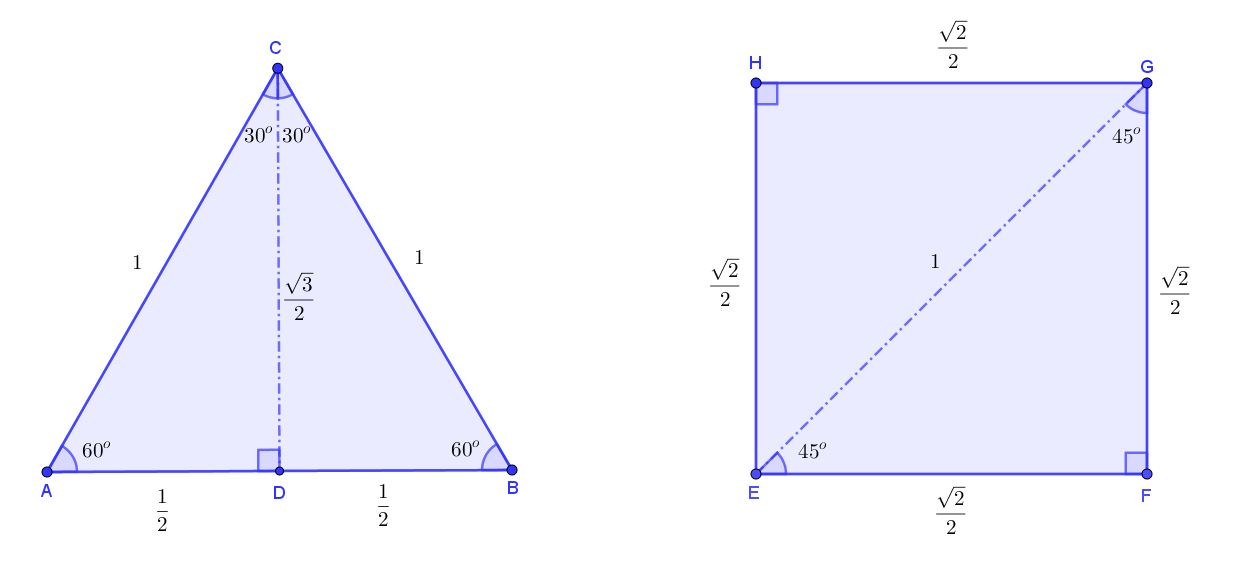
\includegraphics[scale=0.4]{TriangEquil1.JPG}
    \caption{Um triângulo equilátero de lado $1$ e um quadrado de diagonal $1$.}
    \label{TriangEquil1}
\end{figure}

Na \Fref{TriangEquil1}, os  triângulos $ADC$ e $EGH$ são retângulos em $D$ e $H$, respectivamente, e suas hipotenusas medem $1$.

Com auxílio dos triângulos $ADC$ e $EGH$ podemos calcular os valores de seno, cosseno e tangente dos ângulos cujas medidas são $30^\circ, 45^\circ$ e $60^\circ$, chamados de ângulos notáveis. Faça esses cálculos e verifique os valores apresentados na \Tref{table_angulosnotaveis} estão corretos.

\begin{table}[H]
\centering
\begin{tabular}{|c|e{1cm}|e{1cm}|e{1cm}|}
\hline
\tcolor{} &  $\tmat{30^\circ}$ &  $\tmat{45^\circ}$ & $\tmat{60^\circ}$ \tabularnewline 
\hline
$\sen$   & $\frac{1}{2}$ & $\frac{\sqrt{2}}{2}$ & $\frac{\sqrt{3}}{2}$ \tabularnewline
\hline
$\cos$   & $\frac{\sqrt{3}}{2}$ & $\frac{\sqrt{2}}{2}$ & $\frac{1}{2}$ \tabularnewline 
\hline
$\tg$   & $\frac{\sqrt{3}}{3}$ & $1$ & $\sqrt{3}$ \tabularnewline
\hline
\end{tabular}
\caption{Seno, cosseno e tangente dos ângulos notáveis.}
\label{table_angulosnotaveis}
\end{table}

\begin{figure}[H]
    \centering
    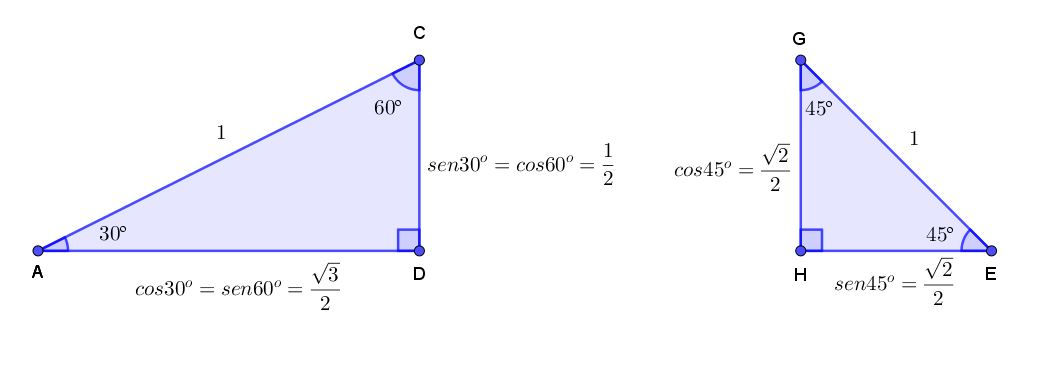
\includegraphics[scale=0.5]{TriagRet4.JPG}
    \caption{Triângulos retângulos $ADC$ e $EGH$.}
    \label{TriagRet4}
\end{figure}
\end{observationtitle}
    
Apesar de ser comum encontrarmos nos livros didáticos muitos problemas que envolvem os ângulos notáveis, vale a pena destacar que eles não são comumente encontrados nos problemas práticos. Nesses casos, como obter os valores do seno, cosseno e tangente destes ângulos? 

Podemos  determinar esses valores de três formas diferentes. A primeira delas consiste em fazer toda a construção que nos levou a definição de seno, cosseno e tangente de um ângulo. Ou seja, neste caso, é necessário construir um triângulo retângulo que possua o ângulo do problema como ângulo interno, e a partir daí, usar os quocientes que definimos anteriormente para calcular seno, cosseno e tangente do ângulo do problema. A segunda forma que temos é utilizar a tabela trigonométrica do final para consultar valores de seno, cosseno e tangente de diversos ângulos. Os valores presentes nessa tabela são obtidos a partir de métodos mais sofisticados que não são tratáveis na Escola Básica. E, uma terceira forma, é utilizando calculadoras, computadores ou telefones celulares, onde esses valores podem ser obtidos de modo imediato.

%%%%%
\know{As origens da Trigonometria}
 
 Geralmente, atribui-se as origens da Trigonometria aos gregos, dada a sua inegável contribuição na sistematização do conhecimento disponível na época, sobretudo com os trabalhos dos matemáticos Euclides, Tales, Pitágoras, entre tantos outros. Segundo \cite{mansfield2017}, foram os babilônios, e não os gregos, os primeiros a estudar Trigonometria, devido a uma placa de argila com $3700$ anos que contempla o assunto. A placa de argila, conhecida pelo nome científico de {\textit {Plimpton 322}}, foi encontrada pelo arqueólogo e acadêmico Edgar Banks no início do século XX, no local que hoje corresponde ao sul do Iraque. Segundo investigadores da Universidade de Nova Gales do Sul, na Austrália, o conteúdo da placa teria sido, possivelmente, usada por matemáticos antigos para fazerem cálculos na construção de palácios, templos e canais.
 
\begin{figure}[H]
    \centering
    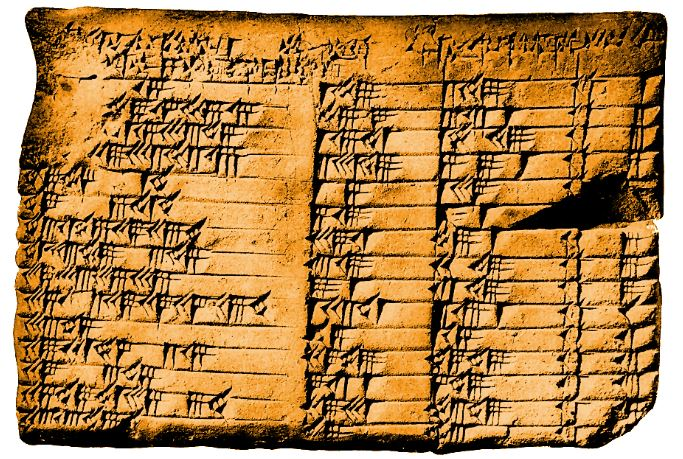
\includegraphics[scale=0.475]{Plimpton.JPG}
    \caption{A placa de argila nomeada {\textit {Plimpton 322}}. Fonte: https://bit.ly/3k1GzVA.}
    \label{Plimpton}
\end{figure}
%https://rcristo.com.br/2018/11/13/conheca-plimpton-322-um-tablete-de-argila-com-escrita-cuneiforme-babilonica-datado-em-3800-anos/

A {\textit {Plimpton 322}}, que a comunidade científica pensa ser proveniente da antiga cidade suméria de Larsa, foi datada do período entre $1822$ a.C. e $1762$ a.C., pertencendo, portanto, à civilização babilônica – o que coloca agora os matemáticos babilônios como os prováveis criadores da Trigonometria, à frente dos gregos.

  
 Apesar de as primeiras noções da Trigonometria serem  bem mais antigas (o grego Hipparchus de Rhodes ($190$ a.C. – $120$ a.C.), considerado o fundador da área, publicou em $180$ a.C. um livro sobre o tema contendo tabelas da primeira função trigonométrica), foi o astrônomo e teólogo alemão Bartholomaeus Pitiscus ($1561$ – $1613$) no seu livro ``Trigonometria: tratado breve e claro da resolução de triângulos'' (em tradução livre do latim), publicado em $1595$, quem mencionou o termo Trigonometria pela primeira vez.  

%%%%% 
\know{Instrumentos de medida}

O ato de medir sempre esteve presente na vida do ser humano, desde os tempos mais remotos. Medir o tamanho de uma propriedade para demarcar terras, a distância entre duas localidades ou entre nosso planeta e astros celestes são exemplos das primeiras medições realizadas por nossos antepassados.

Diante da necessidade de medir objetos ou distâncias, o homem desenvolveu técnicas e instrumentos para realizar tais medidas. Em particular, para realizar suas medições, o homem desenvolveu instrumentos  que foram sendo aprimorados ao longo dos tempos.

Um instrumento de medição muito comum é a trena, como pode ser vista na \Fref{Trena1}. A trena é uma fita ou régua graduada que possui marcações igualmente espaçadas de acordo com alguma unidade de medida. As unidades de medida mais comuns para as trenas são centímetro e metro. Sua forma longa e flexível permite medir objetos longos e curvos. Há registros de que os romanos já possuíam trenas improvisadas por faixas de couro ainda no século VIII a.C.

\begin{figure}[H]
    \centering
    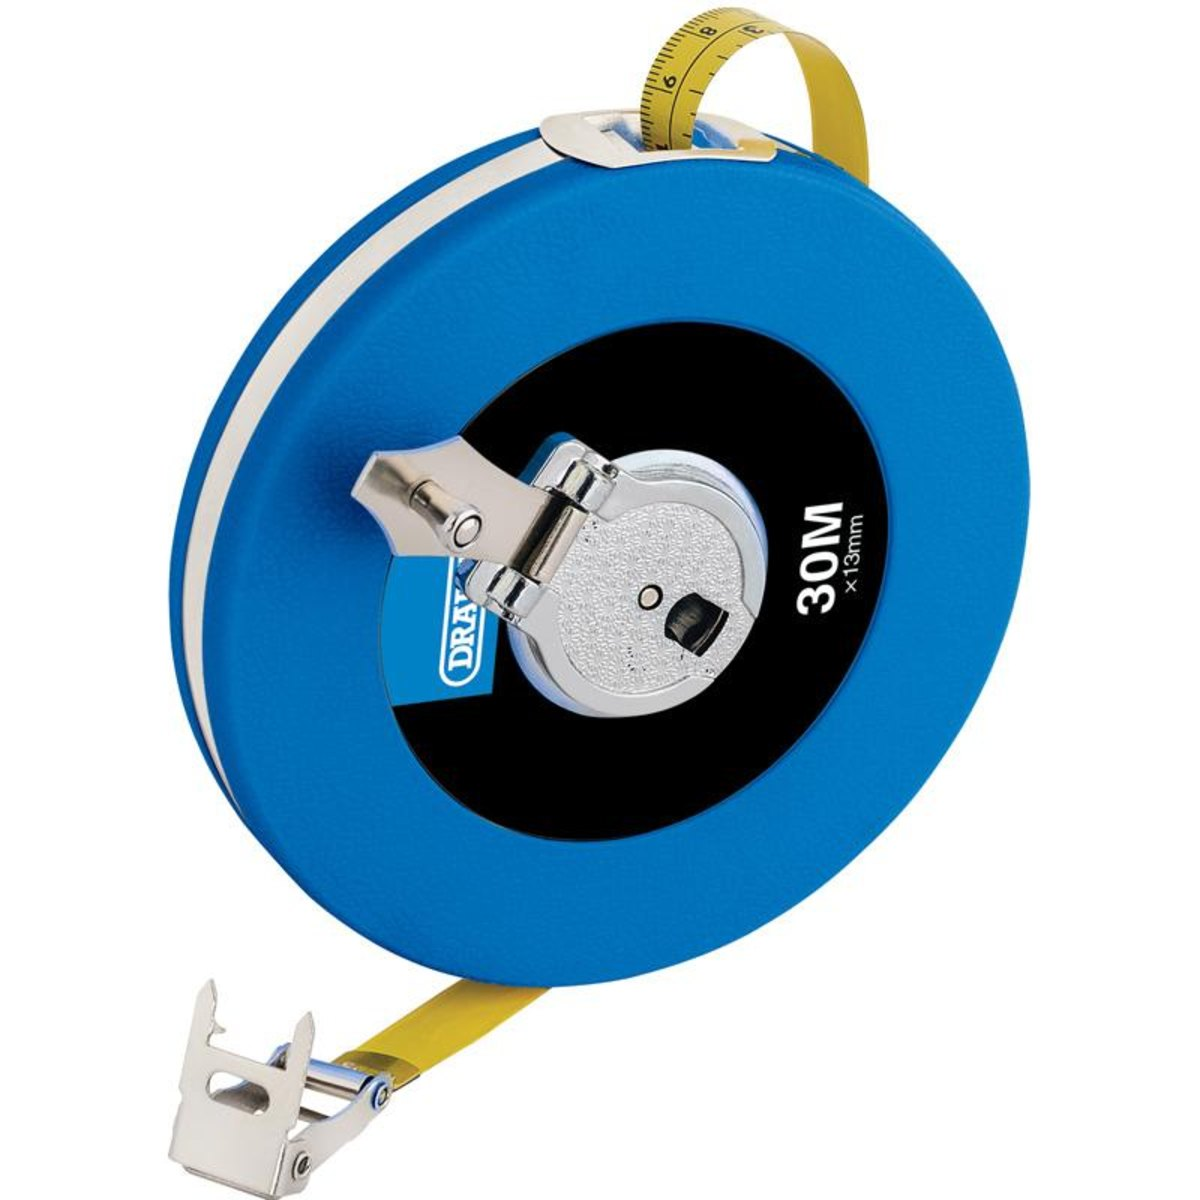
\includegraphics[scale=0.15]{Trena1.jpg}
    \caption{Trena. Fonte: https://bit.ly/2Pc6yvF.}
    \label{Trena1}
\end{figure}
%https://www.google.com/search?q=trena&sxsrf=ALeKk03Af2FHxtDA5MFV_7IkaTwvkJ4shw:1595280956113&source=lnms&tbm=isch&sa=X&ved=2ahUKEwi60dLV5NzqAhWiJ7kGHXucBpIQ_AUoAnoECAwQBA&biw=1920&bih=888#imgrc=P3Kg8LzJ0UHzCM&imgdii=oMl2bqprcH4NsM

Nos dias atuais, são bastante comuns as trenas digitais que podem estimar distâncias utilizando raio laser, além de aplicativos de celulares que utilizam radiações eletromagnéticas para medir distâncias. 

Além de medir distâncias, muito frequentemente temos a necessidade de medir ângulos. Um teodolito é um instrumento ótico que serve para mede ângulos tanto em relação a um plano horizontal pré-fixado, quanto em relação a um plano vertical também pré-fixado. Com o avanço da tecnologia, atualmente, esses instrumentos  oferecem medidas com muita precisão, especialmente nas suas versões digitais. Um teodolito digital pode ser visto na \Fref{Teodolito1}.

\begin{figure}[H]
    \centering
    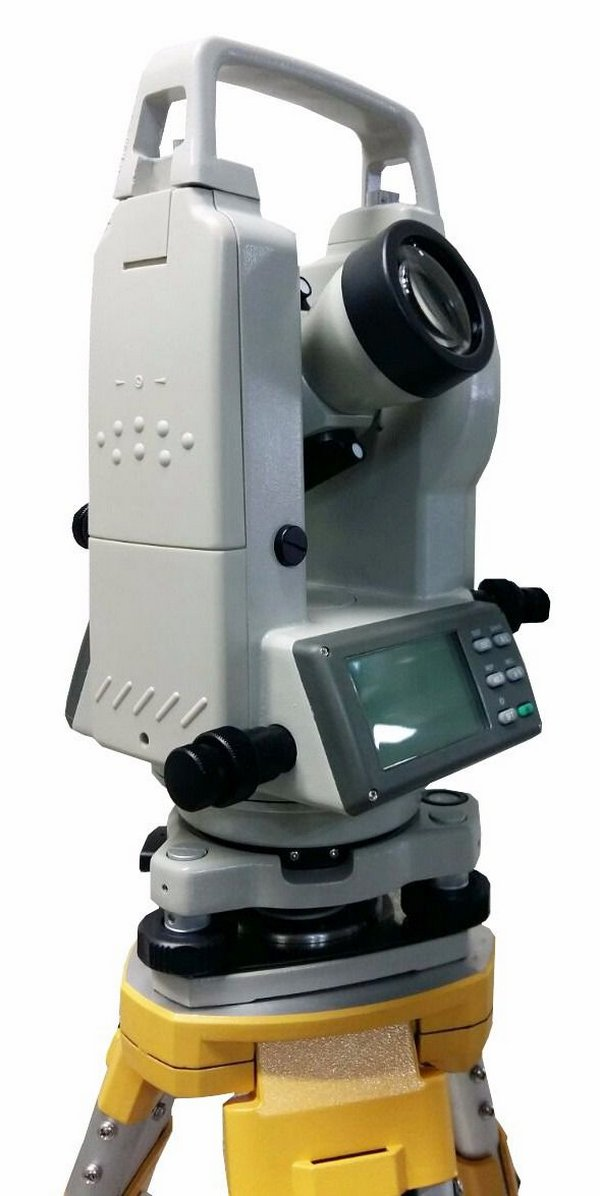
\includegraphics[scale=0.18]{Teodolito1.jpg}
    \caption{Um teodolito digital. Fonte:https://bit.ly/31awZHo.}
    \label{Teodolito1}
\end{figure}
%https://www.google.com/search?q=teodolito&tbm=isch&ved=2ahUKEwiK0_zX5NzqAhUyIrkGHcOkBo8Q2-cCegQIABAA&oq=teodolito&gs_lcp=CgNpbWcQAzIECCMQJzICCAAyAggAMgIIADICCAAyAggAMgIIADICCAAyAggAMgIIADoFCAAQsQM6BAgAEENQ4p4FWIWsBWCpsgVoAHAAeACAAbIBiAH1CpIBAzAuOZgBAKABAaoBC2d3cy13aXotaW1nwAEB&sclient=img&ei=QA4WX4qzPLLE5OUPw8ma-Ag&bih=888&biw=1920#imgrc=ctwUzgB8BZRi-M&imgdii=JYKz0wWOx4FVXM

As trenas, em geral, são muito comuns nas nossas casas, ao contrário do teodolito que é um aparelho mais sofisticado. O teodolito, em geral, é  utilizado por engenheiros, agrimensores, arquitetos e etc. Apesar disso, é possível construir um teodolito caseiro como o da  \Fref{Teodolito2} com materiais caseiros.

\begin{figure}[H]
\centering
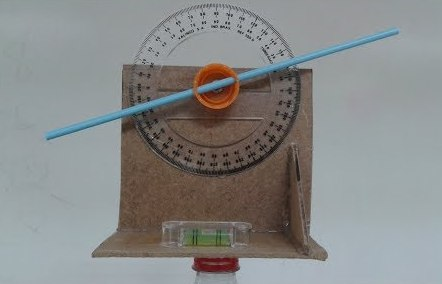
\includegraphics[scale=0.8]{Teodolito2.jpg}
\caption{Um teodolito feito com material caseiro. Fonte:https://bit.ly/2D6uMox.}
\label{Teodolito2}
\end{figure}
\clearpage
\def\currentcolor{session2}
\begin{objectives}{Medindo a altura de uma montanha}
{
\begin{itemize}
\item Utilizar seno, cosseno e tangente de ângulo agudo para resolver situações-problema do mundo real; reconhecer a Trigonometria como uma ferramenta necessária para trabalhar com problemas práticos.

\item \textbf{Conceitos abordados}: triângulos retângulos e razões trigonométricas de um ângulo agudo.
\end{itemize}
}{1}{2}
\end{objectives}
\begin{sugestions}{Medindo a altura de uma montanha}
{
Com a disponibilidade dos recursos digitais dos dias atuais, tais como sites e aplicativos de celulares, um estudante pode, em poucos segundos, responder certas questões que os nossos antepassados investiram um tempo significativo para responder. É preciso conscientizar os estudantes de que apesar da facilidade para responder certas questões proporcionada pelo uso da tecnologia, internamente esses aplicativos utilizam os conceitos desenvolvidos por nossos antepassados, o que justifica a necessidade de entender esses mecanismos e a teoria envolvida. É claro que, na Escola Básica, teremos acesso apenas a parte dos mecanismos e da teoria envolvida.

\textbf{Organização da turma}: individual.

\textbf{Enriquecimento da discussão}: na maioria dos textos que tratam da Trigonometria, as questões são propostas de modo direto, ou seja, são feitas perguntas do tipo ``qual a medida de um certo ângulo ou segmento?'' ou imperativas, tais como ``determine a medida de certo segmento ou ângulo''. Nessa atividade, o aluno será apresentado, de maneira natural, a um determinado problema e será convidado a propor um método para resolvê-lo. Com isso, o aluno terá que elaborar e responder suas próprias questões que, por sua vez, o conduzirão à solução do problema.
}{1}{2}
\end{sugestions}
\begin{answer}{Medindo a altura de uma montanha}
{
No caso específico do Pico do Cabugi, há no seu entorno uma enorme planície, o que facilita o processo de medição da sua altura.  Uma pessoa localizada no ponto $C$ dessa planície em torno da montanha pode, a partir desse ponto, apontar um teodolito na direção do pico da montanha e registrar um ângulo de medida $\theta_1$, conforme ilustra a \Fref{Cabugi2}. Em seguida, essa pessoa, caminhando uma distância $d$ em direção ao pico, chega ao ponto $D$, de onde aponta novamente o teodolito para o pico da montanha; a partir dessa nova posição, o teodolito acusa uma medida $\theta_2$, conforme ilustra a \Fref{Cabugi2}.
\begin{figure}[H]
    \centering
    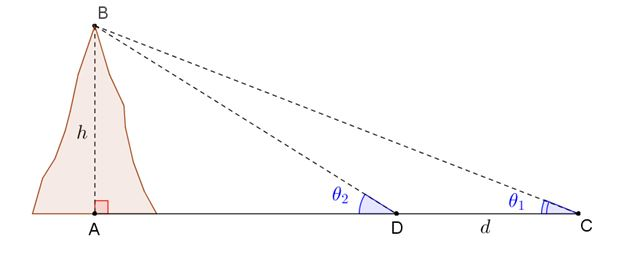
\includegraphics[scale=0.8]{Cabugi2.JPG}
    \caption{Ilustração do Pico do Cabugi.}
    \label{Cabugi2}
\end{figure}

Os seguintes passos levarão à solução do problema:

\begin{itemize}
    \item[$(a)$] No triângulo $ABC$, temos $\tg\theta_1=\frac{h}{AD+d}$.
    \item[$(b)$] No triângulo $ABD$, temos $\tg\theta_2=\frac{h}{AD}$. Assim, os valores desconhecidos são $h$ e $AD$.
    \item[$(c)$] A partir das igualdades encontradas em $(a)$ e $(b)$, vamos isolar $AD$ em ambas as equações e igualar as expressões, obtendo daí uma equação com uma única incógnita $h$. Da igualdade presente em (a), obtemos:
\begin{equation}
\tg\theta_1=\frac{h}{AD+d} \Rightarrow AD+d=\frac{h}{\tg\theta_1}\Rightarrow AD=\frac{h}{\tg\theta_1}-d, \label{um}
\end{equation}
e, da igualdade encontrada em $(b$), temos:
\begin{equation}
\tg\theta_2=\frac{h}{AD} \Rightarrow AD=\frac{h}{\tg\theta_2}. \label{dois}
\end{equation}
Igualando os valores de $AD$ encontrados em \eqref{um} e \eqref{dois}, segue que:
$$\frac{h}{\tg\theta_2}=\frac{h}{\tg\theta_1}-d \Rightarrow h=\left(\frac{\tg\theta_1.\tg\theta_2}{\tg\theta_2-\tg\theta_1}\right)\cdot d.$$
\end{itemize}
    
Assim, podemos determinar a medida da altura do pico em função dos valores $d, \theta_1$  e $\theta_2$  que podem ser encontrados com auxílio de uma trena e de um teodolito caseiro.
    
Apenas por curiosidade, o Pico do Cabugi possui cerca de $590$ metros de altura.
}{9}
\end{answer}
\begin{objectives}{Pitágoras trigonométrico}
{
\begin{itemize}
\item Utilizar as razões trigonométricas de ângulos agudos e áreas de figuras planas para demonstrar o teorema de Pitágoras.
\item \textbf{Conceitos abordados}: razões trigonométricas, áreas e teorema de Pitágoras.
\end{itemize}
}{1}{2}
\end{objectives}
\begin{sugestions}{Pitágoras trigonométrico}
{
\textbf{Organização da turma}: individual.

\textbf{Enriquecimento da discussão}: existem muitas demonstrações do teorema de Pitágoras. Uma das mais antigas é a que está no livro Os Elementos do matemático grego Euclides (Proposição 47, Livro I). Euclides utiliza  equivalência de áreas para demonstrar o teorema de Pitágoras (na verdade, seu enunciado já é uma equivalência de áreas). Essa atividade é uma adaptação da ideia da demonstração realizada por Euclides.

}{1}{1}
\end{sugestions}
\begin{answer}{Pitágoras trigonométrico}
{
\begin{enumerate}
    \item{} 
    No  triângulo retângulo $ABC$, tem-se que:
    $$\cos \alpha=\fra{b}{a} \ \ \text{e} \ \ \cos \beta=\fra{c}{a}.$$
   
    \item{}
    No triângulo $ACL$, $\cos \alpha=\fra{CL}{b} \iff CL=b\cdot\cos \alpha$. Analogamente, no triângulo $ABL$, 
    $\cos \beta=\frac{BL}{c} \iff BL=c\cdot\cos \beta$.
    
    \item{} 
    Ora, $S_1=c^2$ e $S_2=b^2$. Por outro lado, como $\cos \alpha=\frac{b}{a}$ e  $\cos\beta=\frac{c}{a}$, 
    o retângulo $BDJL$ tem lados $BL=c\cdot\cos \beta$ e $BD=a$ e o retângulo $CEJL$ tem lados $CL=b\cdot\cos\alpha$ e $CE=a$, segue que:
    $$\text{Area}(BDJL)=ac\cdot\cos\beta=ac\fra{c}{a}=c^2=S_1,$$
    $$\text{Area}(CEJL)=ab\cdot\cos\alpha=ab\fra{b}{a}=b^2=S_2.$$
    
    \item{}
    Por fim, como $S=a^2$ e $S=S_1+S_2$, segue que:
    $$S=S_1+S_2 \iff a^2=b^2+c^2.$$
\end{enumerate}

Caso tenha acesso a Internet (inclusive de um celular), você pode acessar algumas visualizações da demonstração do teorema de Pitágoras em 
\url{https://www.geogebra.org/m/YA724k8j} e 
\url{https://www.youtube.com/watch?v=CAkMUdeB06o}.
}{1}
\end{answer}
\clearmargin
\begin{objectives}{Largura de uma lagoa}
{
\begin{itemize}
\item Utilizar seno, cosseno e tangente de ângulo agudo para resolver situações-problema do mundo real; reconhecer a Trigonometria como uma ferramenta necessária para trabalhar com problemas práticos.
\item \textbf{Conceitos abordados}: razões trigonométricas de um ângulo agudo e escalas.
\end{itemize}
}{1}{2}
\end{objectives}
\begin{sugestions}{Largura de uma lagoa}
{
Nesta atividade será utilizado o valor de $\tg (85^\circ)=11,43$, que pode ser encontrado na tabela trigonométrica do fim do capítulo. 

\textbf{Organização da turma}: individual,

\textbf{Enriquecimento da discussão}: nessa atividade, o aluno necessitará de régua graduada em centímetros e de um transferidor. O aluno é levado nessa atividade a usar esses instrumentos para resolver um problema real, usando a escala sugerida no mapa. Essa situação problema é interessante, pois mostra como esses instrumentos são úteis e não utilizados apenas para problemas presentes nos livros escolares. Além disso, a atividade põe o aluno numa posição não usual onde ele precisa propor um método ou caminho para resolver um problema.
}{1}{2}
\end{sugestions}
\begin{answer}{Largura de uma lagoa}
{
\begin{enumerate}
 \item{}
Com um teodolito posicionado em $A$, miraríamos o ponto $B$. Em seguida, giraríamos o teodolito sobre o plano horizontal até alcançar um ângulo de $90^\circ$ no sentido horário para quem vê a figura na posição do leitor). Com o teodolito nessa posição, escolheríamos um ponto $C$ de modo que pudéssemos medir a distância $\ell$ de $A$ até $C$, como ilustra a  \Fref{Lagoa2}.
    \begin{figure}[H]
    \centering
    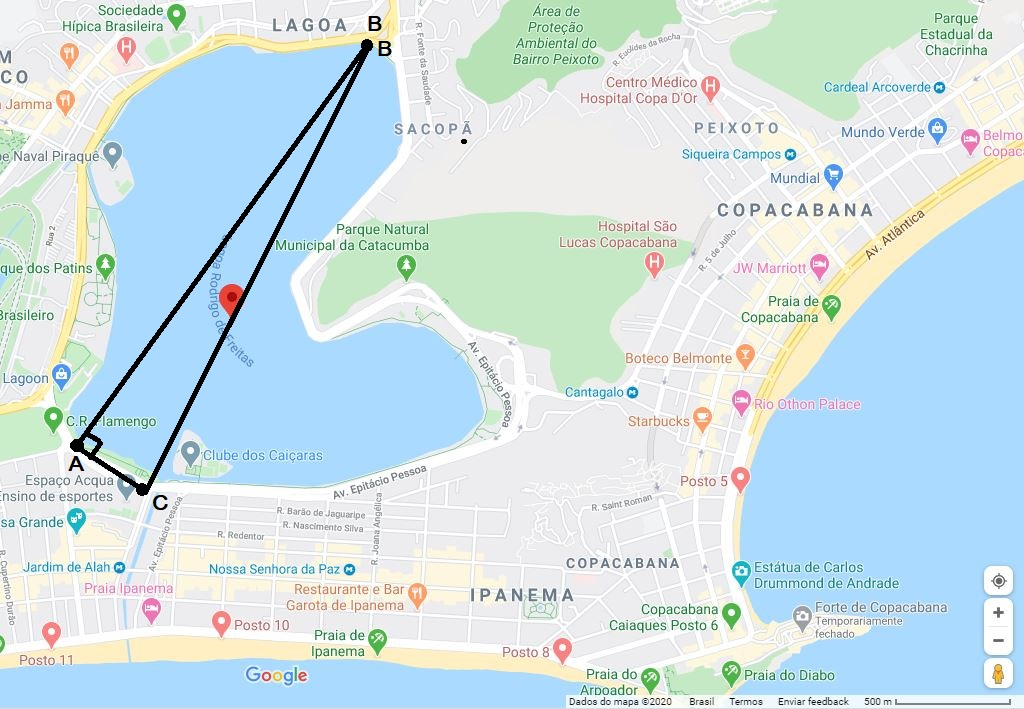
\includegraphics[scale=0.3]{Lagoa2.JPG}
    \caption{Lagoa Rodrigo de Freitas situada na cidade do Rio de Janeiro. Fonte: Google Maps.}
    \label{Lagoa2}
    %Fonte:https://www.google.com.br/maps/place/Lagoa+Rodrigo+de+Freitas/@-22.971588,-43.2178442,15z/data=!3m1!4b1!4m5!3m4!1s0x9bd574afbc853f:0x20a26959ca6918cd!8m2!3d-22.9738464!4d-43.2110285
\end{figure}
Levaríamos o teodolito até o ponto $C$, miraríamos, inicialmente, o ponto $A$ e o giraríamos no sentido horário até o ponto $B$, encontrando o ângulo $A\hat{C}B=\theta$. Sendo assim, $\tg\theta=\frac{d}{\ell} \iff d=\ell\cdot\tg\theta$.

\item{} 
Seguindo o método do item anterior, precisamos utilizar a tangente do ângulo de $85^\circ$ para calcular $d$. Segundo a tabela trigonométrica do final do capítulo, podemos aproximar a tangente de $85^\circ$ por $11,43$, e assim:
$$\tg(85^\circ)=\frac{d}{\ell} \iff d=\ell\cdot\tg(85^\circ) = 200 \cdot 11,43 \approx 2.286\text{m}.$$

\item{} Apoiando a régua sobre o mapa para fazer a medição, encontramos que distância entre os pontos $A$ e $B$ é de aproximadamente $6,7$cm.
   
\item{} Ora, como o segmento de referência da escala possui $1,5$cm (confirme essa medida com a sua régua) e corresponde a uma distância real de $500$m, segue que:
$$\frac{1,5 \text{cm}}{6,7 \text{cm}}=\frac{500 \text{m}}{d} \iff 1,5d=6,7\cdot 500 \iff d \approx 2.233,33 \text{m}.$$

\item{} Usando a escala do Google Maps, a distância estimada entre os pontos $A$ e $B$ é de $2.233,33$m e a estimativa feita com os instrumentos de medida foi de $2.286$m. Entre essas duas estimativas há uma diferença de $2.286  - 2.233,33 =52,67$m. O erro percentual, nesse caso, pode ser obtido da seguinte forma:
$$\frac{2.233,33 \text{m}}{52,67 \text{m}}=\frac{100\%}{x} \iff 2.233,33x=52,67\cdot 100 \iff x\approx 2,35 \%.$$
\end{enumerate}
}{9}
\end{answer}

\practice{Trigonometria no triângulo retângulo}

\begin{task}{Medindo a altura de uma montanha}

Já dissemos que, desde os tempos mais remotos, uma das principais motivações para o desenvolvimento da Trigonometria foi a necessidade de efetuar medições, especialmente obter medidas que fossem inacessíveis diretamente, tais como a medida do raio da Terra, a altura de uma montanha, a largura de um rio, entre outras. Nesta atividade, convidamos você a propor uma possível solução para um problema clássico, supondo que você tenha à mão instrumentos de medidas tais como uma trena e um teodolito caseiro.

No interior do estado do Rio Grande do Norte, uma das montanhas mais famosas é o Pico do Cabugi, localizado no município de Angicos. Sabendo que há uma vasta planície em torno dessa montanha, como você poderia utilizar uma trena e um teodolito para estimar a altura dessa montanha? 

\begin{figure}[H]
    \centering
    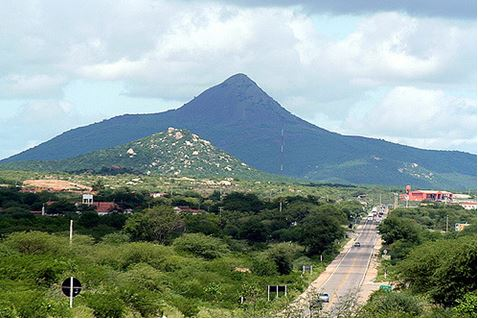
\includegraphics[scale=0.8]{Cabugi1.JPG}
    \caption{Pico do Cabugi,  Angicos - RN. Fonte: https://bit.ly/3lhedri.}
    \label{Cabugi1}
\end{figure}
% Fonte: https://bit.ly/3lhedri
\end{task}

\begin{task}{Pitágoras trigonométrico}
O teorema de Pitágoras, provavelmente, está entre os resultados mais populares de toda a Matemática. O teorema afirma que, num triângulo retângulo $ABC$ cujas medidas da hipotenusa e dos seus catetos são, respectivamente, $a, b$ e $c$, tem-se que $a^2=b^2+c^2$. Geometricamente, isso significa que construindo quadrados sobre a hipotenusa e sobre os catetos deste triângulo retângulo, a área do quadrado sobre a hipotenusa, que nomearemos por $S$, é igual à soma das áreas dos quadrados construídos sobre os catetos, que nomearemos por $S_1$ e $S_2$, conforme ilustra a \Fref{Pitagoras1}.
\begin{figure}[H]
    \centering
    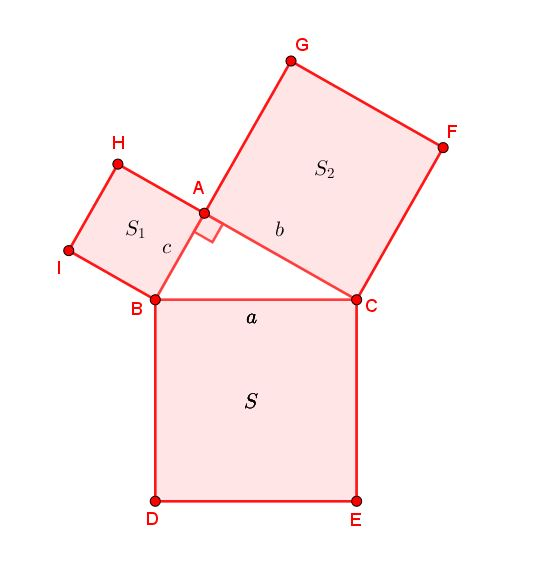
\includegraphics[scale=0.4]{Pitagoras1.JPG}
    \caption{O teorema de Pitágoras: $S=S_1+S_2$.}
    \label{Pitagoras1}
\end{figure}
Ao longo dos tempos, surgiram diversas demonstrações desse teorema. A seguir, vamos utilizar as  razões trigonométricas para deduzí-lo.

\begin{enumerate}
    \item{}
    Sejam $A\hat{C}B=\alpha$ e $A\hat{B}C=\beta$. Determine os valores de $\cos \alpha$ e $\cos \beta$.
    
    \item{}
    Considerando o segmento $AJ$ perpendicular à $DE$, seja $L$ o ponto de interseção de $AJ$ com $BC$, conforme ilustra a \Fref{Pitagoras1.1}.
    \begin{figure}[H]
    \centering
    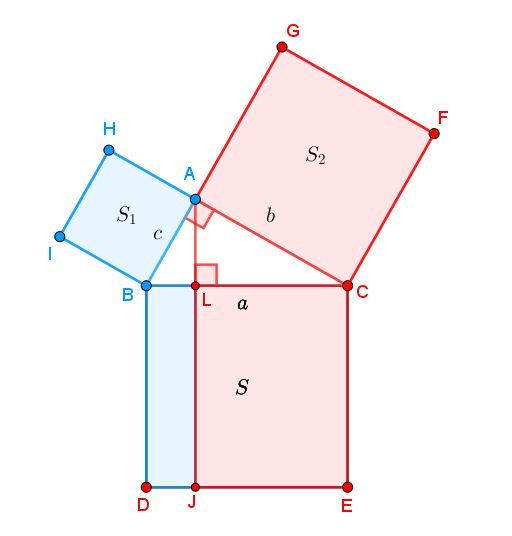
\includegraphics[scale=0.4]{Pitagoras2.JPG}
    \caption{O teorema de Pitágoras: $S=S_1+S_2$.}
    \label{Pitagoras1.1}
\end{figure}
    Obtenha as medidas dos segmentos $BL$ e $CL$ em função das medidas $\alpha, \beta, b$ e $c$.
    
    \item{}
    Qual a relação entre as medidas das áreas dos retângulos $BDJL$ e $CEJL$ e as áreas $S_1$ e $S_2$?
    \item{}
    Usando o fato de que a medida da área do quadrado $BCED$ é igual à soma das medidas dos retângulos $BDJL$ e $CEJL$, conclua que $a^2=b^2+c^2$.
\end{enumerate}
\end{task}

\begin{task}{Largura de uma lagoa}
A \Fref{Lagoa1} mostra uma tela do aplicativo {\textit{Google Maps}} contendo o mapa da região da Lagoa Rodrigo de Freitas situada na cidade do Rio de Janeiro. Nosso objetivo é estimar a distância entre dois pontos fixados na borda dessa lagoa.

Para este exercício, você precisará de uma régua graduada e um transferidor. E caso seja necessário, aproxime valores decimais com duas casas decimais.
\begin{figure}[H]
    \centering
    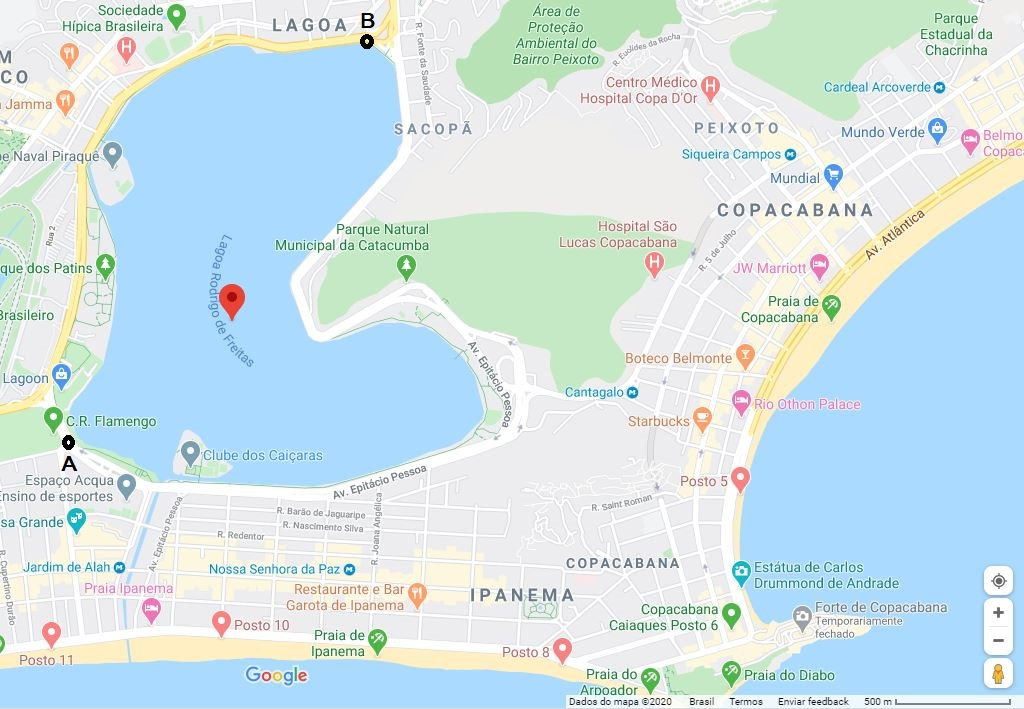
\includegraphics[scale=0.45]{Lagoa1.JPG}
    \caption{Lagoa Rodrigo de Freitas situada na cidade do Rio de Janeiro. Fonte: Google Maps.}
    \label{Lagoa1}
\end{figure}
%Fonte:https://www.google.com.br/maps/place/Lagoa+Rodrigo+de+Freitas/@-22.971588,-43.2178442,15z/data=!3m1!4b1!4m5!3m4!1s0x9bd574afbc853f:0x20a26959ca6918cd!8m2!3d-22.9738464!4d-43.2110285

\begin{enumerate}
\item{}
Na \Fref{Lagoa1}, mostramos os pontos $A$ e $B$ fixados sobre a borda da lagoa. Supondo que você dispusesse de instrumentos de medida adequados (trena e teodolito, por exemplo), proponha um método para estimar a distância $d$ entre esses dois pontos.

\item{}
Seja $C$ um ponto sobre a borda da lagoa tal que $B\hat{A}C=90^\circ$ (medido com o teodolito). Considere ainda que a distância $\ell$ (medida com a trena) entre os pontos $A$ e $C$ seja de $200$m, e que o ângulo $A\hat{C}B$ mede $85^\circ$ (medido com o teodolito). Use o método que você sugeriu no item anterior para estimar um valor para a distância entre os pontos $A$ e $B$.

\item{}
Utilizando uma régua graduada em centímetros e o mapa da \Fref{Lagoa1}, encontre uma estimativa em centímetros para a distância entre $A$ e $B$.

\item{}
No canto inferior direito da \Fref{Lagoa1}, podemos encontrar a escala utilizada para a construção do mapa pelo aplicativo. Neste caso, a escala utilizada é $1,5$cm para representar $500$m. Usando a distância entre os pontos $A$ e $B$ do item anterior, e essa escala, dê uma estimativa para a distância real entre os pontos $A$ e $B$.

\item{}
Tomando a estimativa da distância entre os pontos $A$ e $B$ obtida no item \titem{d)} como referência, qual o erro percentual para a mesma distância que você determinou no item \titem{b)}.
\end{enumerate}
\end{task}

\know{Novamente a medida do raio da Terra}

Adaptamos um texto escrito pelos professores Eduardo Wagner e Marcos Paulo para o Livro Aberto para propor uma nova discussão sobre a medida do raio da Terra.

No início desta seção, discutimos como Eratóstenes determinou com uma excelente precisão a medida do raio terrestre. Agora, utilizando os conceitos estudados nesta seção, vamos mostrar  uma nova forma para estimar a medida do raio da Terra. 
        
Para isso, precisamos levar o teodolito para um lugar alto e que conheçamos sua altura em relação ao nível do mar. Com uma única medição você vai se surpreender com o poder da Trigonometria para resolver esse problema. Mas um pouco de imaginação, ou criatividade, é também necessária!

Vamos considerar a Terra como uma esfera de centro $C$ e raio $R$, e um ponto $P$ situado a uma altura $h$ em relação ao nível do mar. A reta que é definida pelos pontos $C$ e $P$ é dita a reta vertical que passa pelo ponto $P$ e qualquer reta perpendicular a $CP$ é chamada de reta horizontal. Portanto, na \Fref{RaioTerra}, a reta $PX$, perpendicular a $CP$, é uma reta horizontal passando pelo ponto $P$.

   \begin{figure}[H]
    \centering
    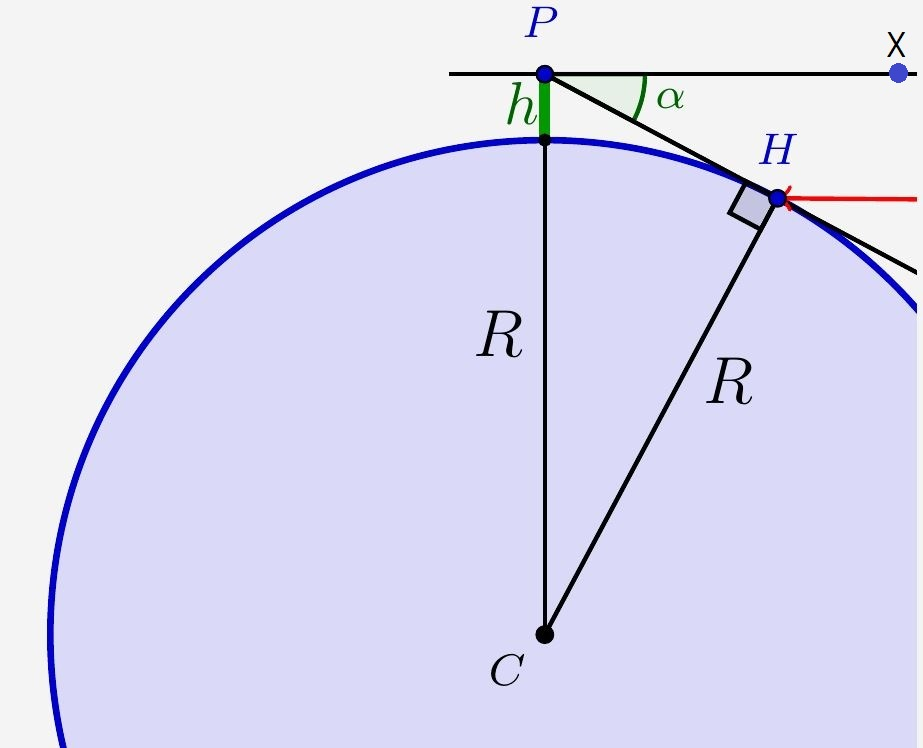
\includegraphics[scale=0.2]{RaioTerra1.JPG}
    \caption{Cálculo da medida do raio da Terra.}
    \label{RaioTerra}
\end{figure}



Considere um teodolito localizado em $P$. Em um dia claro, um observador em $P$ apontando o teodolito na direção $PX$ só vê o céu. Dessa mesma posição, girando ligeiramente o teodolito, ele vê um ponto $H$ sobre a linha do horizonte (diremos que a linha do horizonte é a linha onde o céu encontra o mar). Com auxílio do teodolito, é possível medir o ângulo $X\hat{P}H=\alpha$.

Note que $P\hat{C}H=X\hat{P}H=\alpha$. Assim, no triângulo $PCH$ temos:
\begin{equation}\label{raioT}
\cos\alpha=\frac{R}{R+h} \Rightarrow R=\frac{h\cdot\cos\alpha}{1-\cos\alpha}.
\end{equation}

No Rio de Janeiro, por exemplo, no famoso morro do Corcovado, a base da estátua do Cristo Redentor está aproximadamente $710$m acima do nível do mar. Posicionando o teodolito no pátio do entorno dos pés do Cristo, é possível ver o horizonte em diversas direções. Em uma delas, o teodolito registrou $\alpha=26^\circ$. Como $h=710$m, usando \eqref{raioT}, um valor aproximado para o raio da Terra é 
$$R=\frac{710\cdot\cos(26^\circ)}{1-\cos(26)^\circ}=\frac{710\cdot0,8988}{1-0,8988}\approx 6.305,8102\text{km}.$$

\begin{paginatexto}{Seção 2: Leis da Trigonometria}
Nesta seção, o objetivo é explorar relações entre lados e ângulos pertencentes a triângulos acutângulos e obtusângulos, mostrando ao estudante que podemos ir além do teorema de Pitágoras e das razões trigonométricas dos ângulos agudos exploradas na seção anterior.

Até aqui, as definições de seno, cosseno e tangente de um dado ângulo agudo foram apresentadas apoiadas em uma família especial de triângulos (a saber: triângulos retângulos construídos a partir do ângulo dado); agora, o desafio é transcender o triângulo retângulo e levar o estudante a trabalhar também com ângulos obtusos. 
%
Nesse sentido, esta seção apresentará a definição de seno, cosseno e tangente para ângulos de $0^\circ$ até $180^\circ$. 
%
O professor que sentir necessidade de aprofundamento da discussão acerca desta definição deverá usar o \textit{Para Saber+ Explorando Senos e Cossenos}.

O estudante também será apresentado nesta seção a dois resultados muito importantes da Trigonometria. 
%
São eles: Lei dos Cossenos e Lei dos Senos.
%
Estes dois resultados serão demonstrados e sua importância será comprovada através de uma seleção de problemas de diversos contextos.
%
As demonstrações das duas leis serão apresentadas sempre para os três tipos possíveis de triângulos: retângulo, acutângulo e obtusângulo, e, caberá ao professor decidir se deve ou não abordar as demonstrações em sua aula, podendo optar também por apenas algumas delas.

Em geral, os livros didáticos fazem uso do círculo trigonométrico para definir seno, cosseno e tangente de um ângulo qualquer.
%
A proposta deste capítulo não é usar este tipo de estratégia, mas apenas trabalhar com os ângulos internos de um triângulo qualquer (portanto, entre $0^\circ$ e $180^\circ$).
%
Deixaremos a abordagem do círculo trigonométrico, a definição de radiano e outros conceitos relacionados para o capítulo que abordará as funções trigonométricas.

Sobre a linguagem usada em sala de aula, sugerimos que os estudantes sejam incentivados a usar o vocabulário adequado no contexto de triângulos, em especial, em relação a sua classificação. 
%
Percebemos, em nossa prática docente, que triângulos retângulos são comumente chamados de retângulos, enquanto triângulos acutângulos ou obtusângulos são comumente chamados, apenas, de triângulos.
%
A familiaridade com os termos adequados permitirá que o estudante leia o texto com maior fluidez e compreenda melhor o conteúdo.

No decorrer da seção, frequentemente será necessário calcular seno, cosseno e tangente de ângulos não notáveis, ainda que agudos. 
%
Para estes casos, sugerimos utilizar a tabela trigonométrica disponibilizada no final do capítulo. %
Com o auxílio desta tabela, o estudante poderá obter aproximações dos valores do seno, cosseno e tangente de diversos ângulos e também poderá encontrar o ângulo que possui um determinado valor de seno ou cosseno ou tangente inspecionando a tabela. Neste segundo caso, em especial, evitaremos fazer qualquer menção às funções trigonométricas inversas, que não fazem parte do escopo deste capítulo.
%
Caso seja possível utilizar formas eletrônicas para os cálculos que envolvem ângulos não notáveis, o professor também poderá optar por utilizá-los.
\end{paginatexto}

\def\currentcolor{session1}
\begin{objectives}{Explorando um triângulo não retângulo}
{
\begin{itemize}
\item Trabalhar com o teorema Pitágoras, reafirmando sua aplicabilidade apenas para triângulos retângulos; desenvolver uma relação métrica válida em um triângulo obtusângulo que dará origem, mais adiante, à lei dos cossenos.
\item \textbf{Conceitos abordados}: relações métricas em triângulos retângulos.
\end{itemize}
}{1}{1}
\end{objectives}
\begin{sugestions}{Explorando um triângulo não retângulo}
{

Para esta atividade, o estudante deverá utilizar uma régua para fazer as construções pedidas.

\textbf{Organização da turma}: em duplas ou pequenos grupos para que os alunos possam se envolver nas discussões propostas.

\textbf{Dificuldades previstas}: é muito comum que os estudantes usem o teorema de Pitágoras em um triângulo qualquer, não atentando para o fato de sua validade estar ligada ao triângulo ser retângulo. Sugerimos ao professor ficar atento a este distrator e corrigir erros relacionados, caso apareçam, aproveitando a situação para uma revisão do conteúdo já estudado.

\textbf{Enriquecimento da discussão}: esta atividade pretende despertar o interesse do aluno na busca por um resultado que estenda o teorema de Pitágoras para triângulos quaisquer. Provavelmente, o aluno nunca foi levado a questionar essa possibilidade; com essa atividade, pretendemos que ele comece a desconfiar da existência de algum resultado ainda por ele desconhecido. Além disso, sugerimos ao professor que permita e incentive o aluno a se expressar livremente e que aproveite a oportunidade para ajudá-lo a refinar seu vocabulário no contexto dos triângulos (tipos, ângulos internos e externos, ângulos complementares e suplementares, altura e etc).  
}{1}{1}
\end{sugestions}
\begin{answer}{Explorando um triângulo não retângulo}
{
\begin{enumerate}
    \item{}
    Na  \Fref{sec2_trignaoret_resl_fig}, apresentamos uma possível construção para o triângulo $ABC$. Independentemente da construção realizada, o triângulo $ABC$ não é retângulo. Como o ângulo $B\hat{A}C$ é obtuso, então os demais ângulos internos desse triângulo possuem medida menor que $90^\circ$. Do contrário, as medidas dos ângulos internos de $ABC$ não somariam $180^\circ$.
    
    \begin{figure}[H]
    \centering
    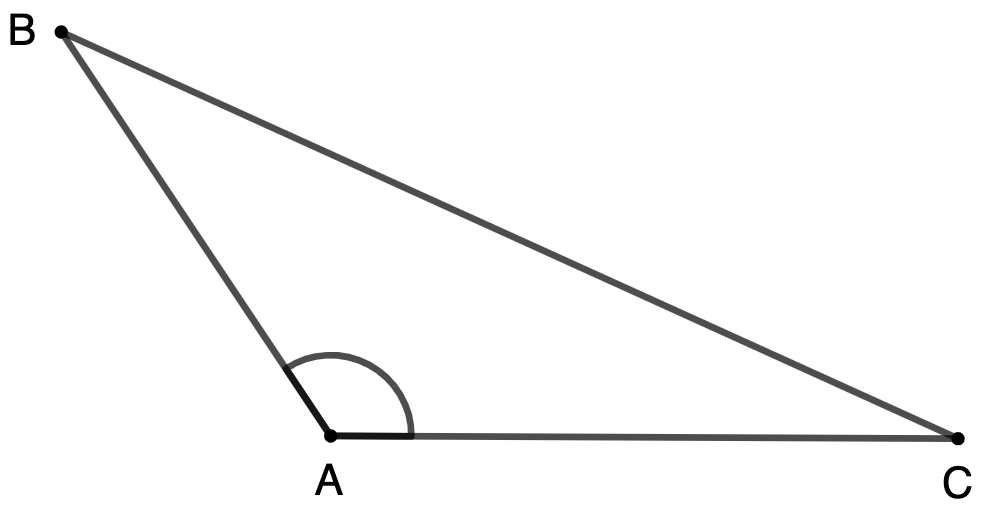
\includegraphics[scale=0.6]{sec2_explorando_trig_nao_ret_res1.png}
    \caption{Triângulo não retângulo $ABC$.}
    \label{sec2_trignaoret_resl_fig}
\end{figure}
    
    \item{}
    Na \Fref{sec2_trignaoret_res2_fig}, $BD$ é a  altura do triângulo $ABC$ traçada a partir de $B$. Neste caso, como o ângulo $B\hat{A}C$ é obtuso, a altura $BD$ é externa ao triângulo.
    \begin{figure}[H]
    \centering
    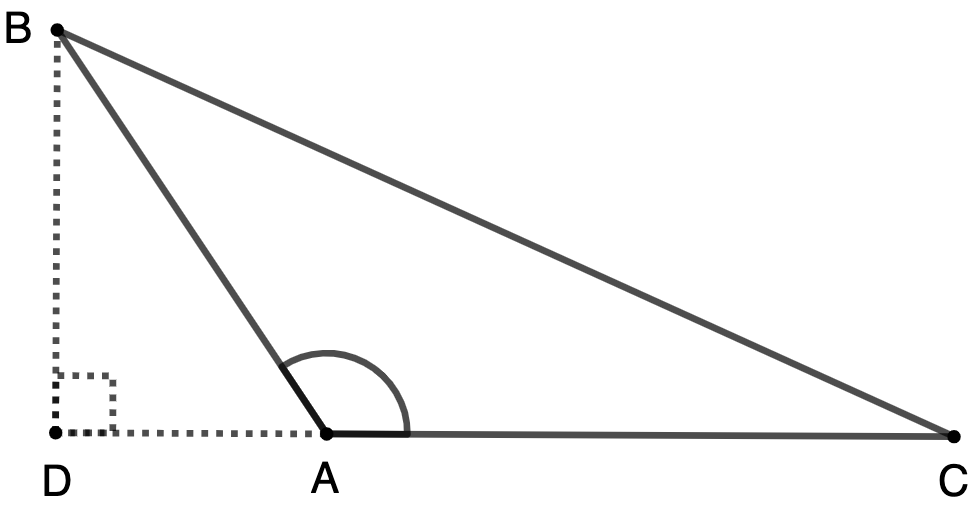
\includegraphics[scale=0.6]{sec2_explorando_trig_nao_ret_res2.png}
    \caption{Altura $BD$ do triângulo $ABC$ a partir de $B$.}
    \label{sec2_trignaoret_res2_fig}
\end{figure}
    
    \item{}
    Neste item, usaremos a  \Fref{sec2_trignaoret_res3_fig} que contém a notação apresentada no enunciado.
   
    Aplicando o teorema de Pitágoras no triângulo $DBA$ retângulo em $D$, obtemos 
    \begin{equation}
     c^2=h^2+u^2.   \label{sec2_at_trignaoret_eq1}
    \end{equation}
    
    Agora, fazendo o mesmo cálculo para o triângulo $DBC$ retângulo em $D$, obtemos 
    \begin{equation}
     a^2=h^2+(u+b)^2.   \label{sec2_at_trignaoret_eq2}
    \end{equation}
    \begin{figure}[H]
    \centering
    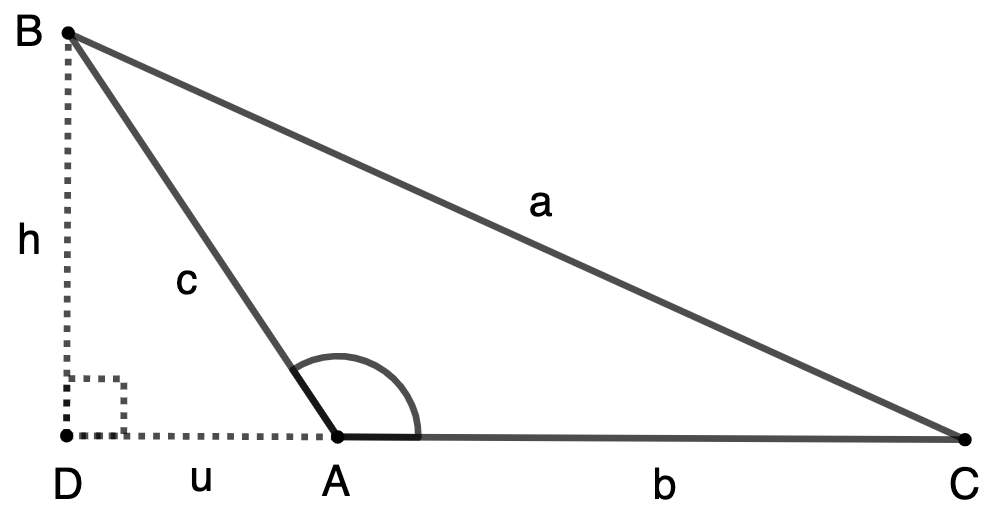
\includegraphics[scale=0.6]{sec2_explorando_trig_nao_ret_res3.png}
    \caption{Triângulo $ABC$ e sua altura $BD$.}
    \label{sec2_trignaoret_res3_fig}
\end{figure}
    
    \item{}
    O triângulo $ABC$ não é retângulo, portanto não podemos usar o teorema de Pitágoras para encontrar uma relação como a encontrada no item anterior para os triângulos $DBA$ e $DBC$, que são retângulos. 
    
    Neste caso, como pede o enunciado, vamos encontrar uma relação envolvendo $a, b, c$ e $u$ para o triângulo $ABC$. Para isso, de \eqref{sec2_at_trignaoret_eq1} temos que $h^2=c^2-u^2$. Substituindo essa igualdade em \eqref{sec2_at_trignaoret_eq2}, vemos que
    $$a^2=c^2-u^2+u^2+2bu+b^2 \iff a^2=b^2+c^2+2bu,$$
    
    que é a relação pedida.
    
    \item{}
    As relações provenientes da aplicação do teorema de Pitágoras aos triângulos retângulos $DBA$ e $DBC$ envolvem apenas as medidas dos lados dos triângulos, enquanto que a relação obtida no item anterior utiliza (além das medidas dos lados) uma medida $u$ externa ao triângulo, mas determinada por ele. 
    
    Para responder a segunda pergunta, é necessário buscar uma forma de expressar $u$ em termos dos dados do triângulo. Veremos mais adiante que, para isso, precisaremos envolver os ângulos do triângulo. 
\end{enumerate}
}{9}
\end{answer}
\clearmargin
\begin{objectives}{Desenvolvendo um jogo de futebol para videogame}
{
Perceber a necessidade de estender para triângulos não necessariamente retângulos a teoria já estudada, indo além do teorema de Pitágoras; aplicar a argumentação utilizada na demonstração da lei dos cossenos, que será sistematizada adiante, na solução de um problema numérico e adquirir familiaridade com este tipo de argumentação antes dela ser utilizada.  

\textbf{Conceitos abordados}: razões trigonométricas de um ângulo agudo.
}{1}{2}
\end{objectives}
\begin{sugestions}{Desenvolvendo um jogo de futebol para videogame}
{
Nesta atividade serão utilizados os seguintes dados, que poderão ser acessados pelos estudantes na tabela trigonométrica do fim do capítulo: $\arcsen({0,82}) = 55^\circ, \arcsen({0,089}) = 5^\circ$ e $\arccos({0,98})=10,29^\circ$. Para encontrar o ângulo que possui determinado valor de seno e cosseno, será necessário utilizar a tabela de maneira contrária à tradicional (quando queremos encontrar o valor de seno e cosseno de um dado ângulo). Ou seja, o estudante deverá procurar na coluna seno e cosseno o valor encontrado na atividade e então, identificar na coluna dos ângulos qual o ângulo relacionado ao dado valor de seno e cosseno. É importante lembrar que, como já foi dito anteriormente, o professor não deve utilizar a linguagem e nomenclatura de função trigonométrica inversa em sua sala de aula. Destacamos esses dados, neste momento, para informar ao professor o que será utilizado na atividade e com o intuito de auxiliá-lo na manipulação da tabela.

\textbf{Organização da turma}: em duplas ou pequenos grupos para que os alunos possam ter espaço para se envolver nas discussões propostas.

\textbf{Enriquecimento da discussão}: essa atividade deve ser usada para destacar novamente que o teorema de Pitágoras só é válido para triângulos retângulos e para guiar o estudante a concluir que uma ampliação deste teorema necessariamente deve envolver também algum dos ângulos do triângulo, diferentemente do teorema de Pitágoras. É muito importante que o professor guie e fomente a discussão em torno dessas questões.
}{1}{2}
\end{sugestions}
\clearmargin
\mspace{.25em}
\begin{answer}{Desenvolvendo um jogo de futebol para videogame}
{\paragraph{Parte I}

\begin{enumerate}\small
    % 

    \item Visualmente, provavelmente, será difícil decidir qual ângulo é o maior. Entretanto, nesse item podemos incentivar que os estudantes conversem, discutam e conjecturem entre si.
    
    \item{}
    Vamos primeiramente calcular o ângulo do chute ao gol do jogador $A$. Como o triângulo $AT_1T_2$ não é um triângulo retângulo, não podemos usar o teorema de Pitágoras diretamente, tão pouco as razões trigonométricas aprendidas na seção anterior. Vamos então, buscar triângulos retângulos presentes na situação para aplicarmos a teoria que conhecemos, e indiretamente calcular o ângulo procurado.
    
    Vamos usar a \Fref{sec2_futebol_res1_fig} para nos auxiliar nesse item. Seja $M$ o ponto posicionado sobre a junção das linhas que delimitam o campo de futebol.

    \notas{
\adjustbox{valign=t}
{
        \begin{minipage}{\linewidth}
        \begin{figure}[H]
                \centering
                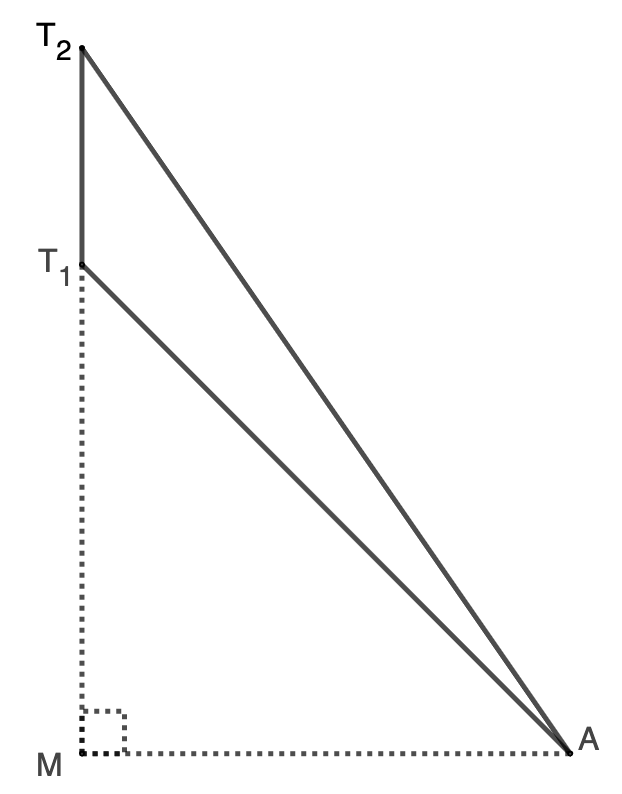
\includegraphics[scale=0.3]{sec2_trig1_atfutebol.png}
                \caption{Triângulo $AT_1T_2$. (Atividade \hyperref[desenvolvendo-jogo]{Desenvolvendo um jogo de futebol para videogame})}
                \label{sec2_futebol_res1_fig}
            \end{figure}
        \end{minipage}
}
        }

    Note que o triângulo $MAT_1$ é retângulo em $M$ e isósceles, já que $AM$ e $MT_1$ são congruentes (ver \Fref{sec2_futebol4_fig}). Sendo assim, o ângulo $M\hat{A}T_1$ mede $45^\circ$. Além disso, como $MAT_2$ é retângulo (e não isósceles, já que este triângulo não possui dois lados congruentes), então 
    $$\sen(M\hat{A}T_2)=\frac{MT_2}{AT_2}=\frac{16,5+7,3}{28,96}=0,821.$$
    Neste caso, o resultado foi aproximado utilizando duas casas decimais.
    
    Com o auxílio da tabela trigonométrica do final do capítulo, é possível determinar que $M\hat{A}T_2$ mede aproximadamente $55^\circ$. Portanto, $T_1\hat{A}T_2=M\hat{A}T_2-M\hat{A}T_1$ mede aproximadamente $55^\circ-45^\circ=10^\circ$.
    
    Sendo assim, o jogador $A$ possui um ângulo certeiro ao gol de aproximadamente $10^\circ$.
    
    \notas{
\adjustbox{valign=t}
{
        \begin{minipage}{\linewidth}
        \begin{figure}[H]
            \centering
            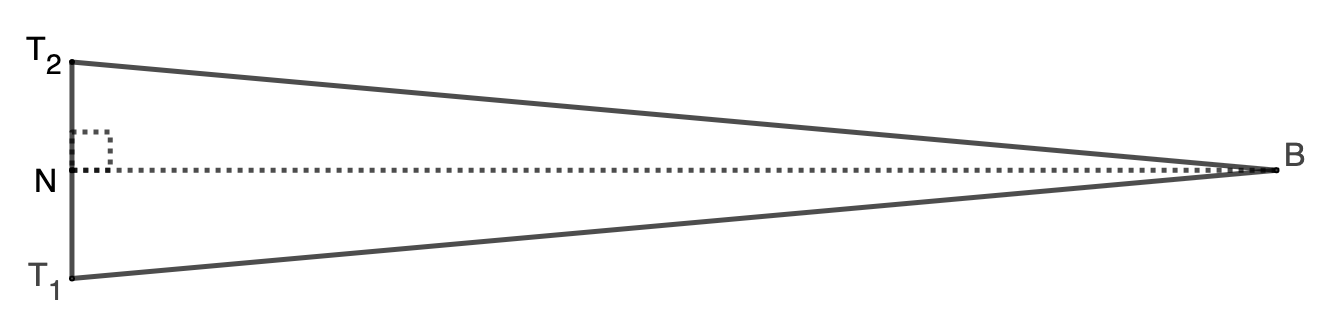
\includegraphics[scale=0.2]{sec2_trig2_atfutebol.png}
            \caption{Triângulo $BT_1T_2$. (Atividade \hyperref[desenvolvendo-jogo]{Desenvolvendo um jogo de futebol para videogame})}
            \label{sec2_futebol_res2_fig}
        \end{figure}
        \end{minipage}
}
        }
    
    Trabalhando com a situação do jogador $B$, ilustrada na \Fref{sec2_futebol_res2_fig}, nos deparamos com um triângulo isósceles $BT_1T_2$. Marque $N$ como sendo o pé da perpendicular baixada de $B$ sobre $T_1T_2$. Dessa forma, $BN$ é a altura do triângulo em relação à base $T_1T_2$, que também é a bissetriz do ângulo $B$. Assim,
    $$\sen(N\hat{B}T_1)=\sen(N\hat{B}T_2)=\fra{NT_1}{BT_1}=\fra{3,65}{40,82}=0,089.$$
    Novamente com o auxílio da tabela trigonométrica do final do capítulo, concluímos que $N\hat{B}T_1$ e $N\hat{B}T_2$ medem aproximadamente $5^\circ$. Portanto, $T_1\hat{B}T_2$ mede aproximadamente $10^\circ$.
    
    Pelos cálculos acima, o jogador $B$ possui um ângulo certeiro ao gol de $10^\circ$.
    
    Nos casos dos dois jogadores $A$ e $B$, utilizamos aproximações com três casas decimais para medir distâncias e calcular o valor de seno do ângulo. Podemos, então, concluir que os jogadores $A$ e $B$ possuem, aproximadamente, o mesmo ângulo certeiro ao gol. 
\end{enumerate}
}{1}
\end{answer}

\clearmargin
\mspace{.25em}
\begin{answer}{Desenvolvendo um jogo de futebol para videogame}
{
\begin{enumerate}
\item Visualmente, provavelmente, será difícil decidir qual ângulo é o maior, mas como no primeiro item desta atividade, devemos incentivar os estudantes a se expressarem e conjecturarem sobre a situação. 
    
    \item{}
    Vamos utilizar a \Fref{sec2_futebol_res3_fig} para resolver esse item. Na situação mostrada na figura, marcamos o ponto $O$ como sendo o pé da perpendicular baixada de $T_2$ até $T_1C$. Logo, $OT_2$ é a altura do triângulo $T_1CT_2$ em relação ao lado $T_1C$. 

    \notas
    {
    \adjustbox{valign=t}
    {
    \begin{minipage}{\linewidth}
        \begin{figure}[H]
            \centering
            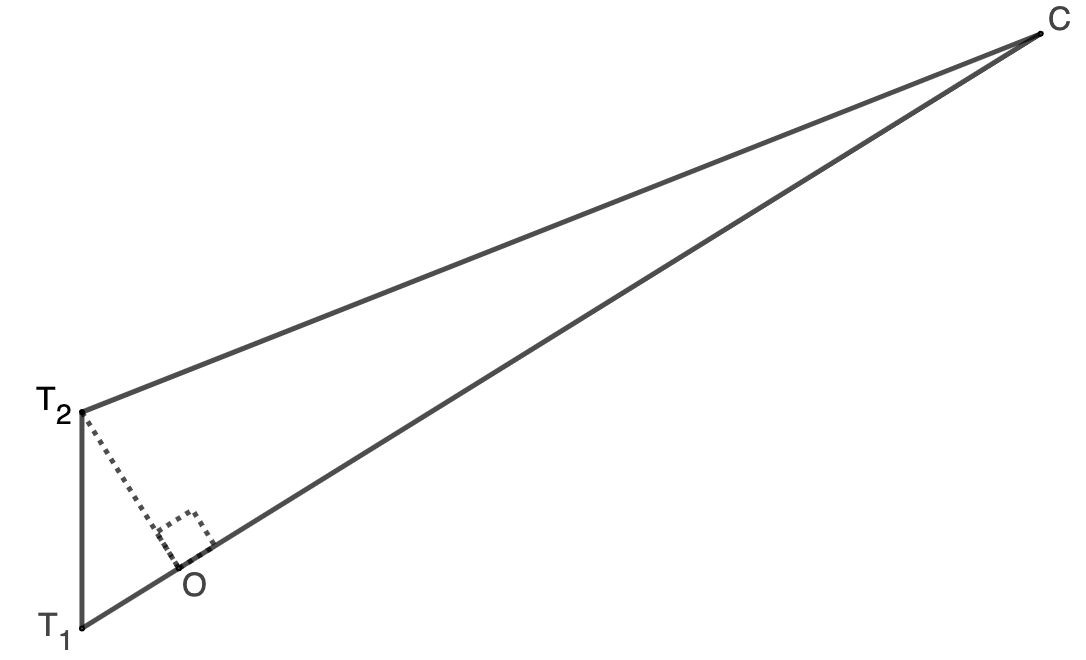
\includegraphics[scale=0.4]{sec2_trig3_atfutebol.png}
            \caption{Triângulo $CT_1T_2$. (Atividade \hyperref[desenvolvendo-jogo]{Desenvolvendo um jogo de futebol para videogame})}
            \label{sec2_futebol_res3_fig}
        \end{figure}
    \end{minipage}
    }
    }
     
    Como $OCT_2$ é um triângulo retângulo, temos
    $$\sen(\hat{T_2CT_1})=\fra{OT_2}{CT_2}\;\; \text{ e } \;\; \cos(\hat{T_2CT_1})=\fra{CO}{CT_2}.$$
    
    Logo,
    \begin{eqnarray}
    OT_2=CT_2 \cdot \sen(\hat{T_2CT_1}),\label{sec2_futebol_res_eq1}\\
    CO=CT_2 \cdot \cos(\hat{T_2CT_1}).\label{sec2_futebol_res_eq2}
    \end{eqnarray}
    De \eqref{sec2_futebol_res_eq2}, temos que
    \begin{equation}
        OT_1=T_1C-CT_2\cdot\cos(\hat{T_2CT_1}).\label{sec2_futebol_res_eq3}
    \end{equation}
    Agora, observando que $OT_1T_2$ é um triângulo retângulo em $O$, podemos usar o teorema de Pitágoras:
    $$T_1T_2^2=OT_1^2+OT_2^2.$$
    
    Utilizando as equações \eqref{sec2_futebol_res_eq1} e \eqref{sec2_futebol_res_eq3} na equação acima, temos
    $$T_1T_2^2=(T_1C-CT_2\cdot\cos(\hat{T_2CT_1}))^2+(CT_2\cdot\sen(\hat{T_2CT_1}))^2$$
    que implica
    $$7,3^2=38,08^2-2\cdot 38,08\cdot 34,79\cdot \cos(\hat{T_2CT_1})+34,79^2.$$
    Resolvendo a equação acima encontramos $\cos(\hat{T_2CT_1})=0,983$, e usando a tabela trigonométrica, podemos concluir que o ângulo $\cos(\hat{T_2CT_1})$ mede aproximadamente $10^\circ$.
     
    Considerando novamente todas as aproximações feitas, podemos concluir então, que os jogadores $A,B$ e $C$ possuem, aproximadamente, o mesmo ângulo certeiro ao gol. 
      
    \item{}
    Sim, é possível calcular o ângulo em todos os casos. Para isso, basta seguir o procedimento do item anterior, sem nenhuma informação adicional.
\end{enumerate}
}{1}
\end{answer}
\clearmargin
\begin{answer}{Desenvolvendo um jogo de futebol para videogame}
{
\paragraph{Parte II}
\begin{enumerate}
  \item{}
     Preenchendo a tabela pedida, temos:
     \begin{table}[H]
\centering
\begin{tabular}{|c|c|c|c|}
\hline
\tcolor{Jogador} & $\tmat{\quad a \quad}$ & $\tmat{\quad b \quad}$ & $\tmat{\quad c \quad}$ \\ %
\hline                               
A & 7,3 & 23,33 & 28,96 \\
\hline
B & 7,3 & 40,82 & 40,82 \\
\hline
C & 7,3 & 38,08 & 34,79 \\
\hline
\end{tabular}
\caption{Dados dos jogadores $A, B$ e $C$.}
\label{sec2_tabfutebol_res1}
\end{table}

     \item{}
     Preenchendo a tabela pedida, temos os seguintes valores aproximados:
     \begin{table}[H]
\centering
\begin{tabular}{|c|c|c|c|e{3cm}|}
\hline
\tcolor{Jogador} & $\tmat{\quad a \quad}$ & $\tmat{\quad b \quad}$ & $\tmat{\quad c \quad}$ & \tcolor{$\quad  \dfrac{\bm{b^2+c^2-a^2}}{\bm{2bc}} \quad$} \tabularnewline %\hline                               
$A$ & $7{,}3$ & $23{,}33$ & $28{,}96$ & $0{,}984$ \tabularnewline
\hline
$B$ & $7{,}3$ & $40{,}82$ & $40{,}82$ & $0{,}984$ \tabularnewline
\hline
$C$ & 7{,}3 & $38{,}08$ & $34{,}79$ & $0{,}984$ \tabularnewline
\hline
\end{tabular}
\caption{Dados dos jogadores $A, B$ e $C$.}
\label{sec2_tabfutebol_res2}
\end{table}

\item{}
Por esta tabela, percebemos que a expressão $\frac{b^2+c^2-a^2}{2bc}$ gera valores aproximadamente iguais para os triângulos $AT_1T_2, BT_1T_2$ e $CT_1T_2$. Isto nos permite conjecturar que há alguma relação entre os lados dos três triângulos que envolve algo que não se altera nesses três triângulos, mesmo sendo estes diferentes. Lembrando o que encontramos na PARTE I desta atividade, provavelmente esta terceira coluna expressa algo relacionado ao ângulo do chute certeiro ao gol, que é aproximadamente igual para os três jogadores. Isso será explicado com detalhes a seguir.
 \end{enumerate}
}{1}
\end{answer}

\explore{Indo além do teorema de Pitágoras}\label{exp_estendenoteopitagoras}


No Ensino Fundamental, estudamos algumas relações métricas do triângulo retângulo, como o teorema de Pitágoras. 
%
O amplo uso desses resultados no estudo dos mais diversos problemas geométricos mostra sua relevância e importância para a Geometria.

Como sabemos, o teorema de Pitágoras é um teorema válido apenas para triângulos retângulos. 
%
Mas, então, será que existe um resultado similar ao teorema de Pitágoras válido para um triângulo qualquer? 
%
Ou seja, existe um teorema que relacione a medida dos lados de um triângulo qualquer? 
%
Com o auxílio das relações trigonométricas estabelecidas neste capítulo, iremos juntos buscar uma resposta para esse questionamento.


\begin{task}{Explorando um triângulo não retângulo}
Nesta atividade, você precisará de uma régua para fazer as construções pedidas.

A partir do ângulo obtuso com vértice em $A$ da \Fref{sec2_explorando_trig_nao_ret_fig}, construa um triângulo $ABC$ de forma que o vértice $C$ esteja sobre o lado horizontal do ângulo obtuso dado e $B$ sobre o outro lado. 

Utilizando o triângulo $ABC$ que você construiu, faça o que se pede a seguir.
\begin{figure}[H]
    \centering
    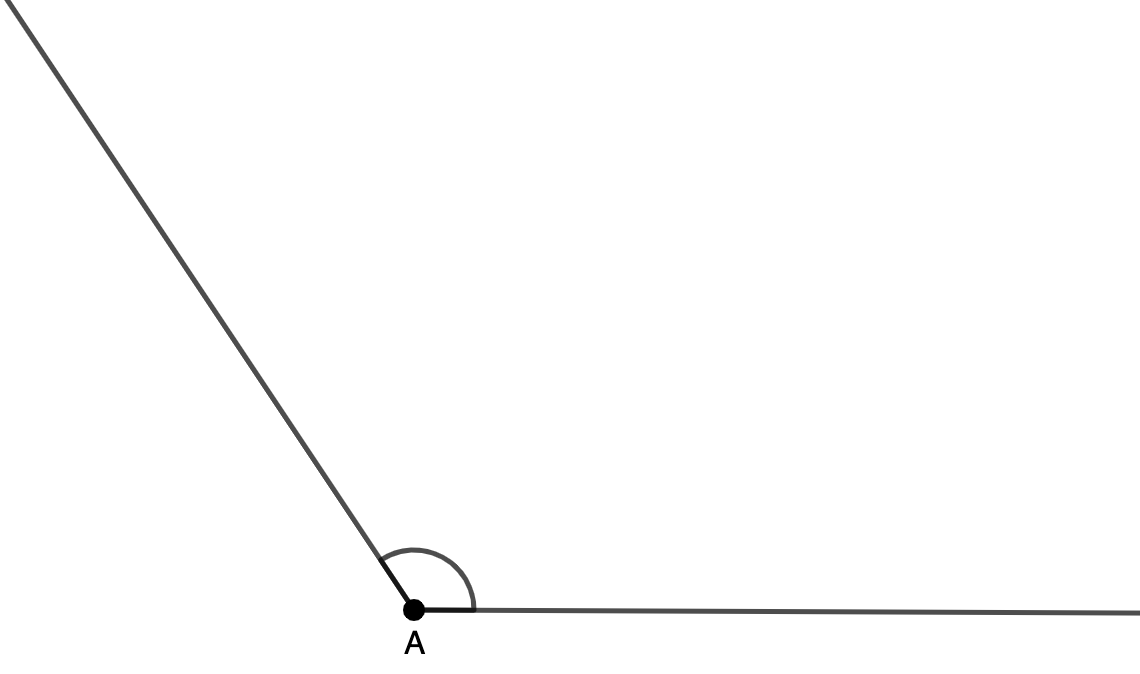
\includegraphics[scale=0.35]{sec2_explorando_trig_nao_ret1.png}
    \caption{Ângulo obtuso com vértice em $A$.}
    \label{sec2_explorando_trig_nao_ret_fig}
\end{figure}

\begin{enumerate}
    \item{}
    O triângulo $ABC$ que você construiu é retângulo? Por que?
    
    \item{}
    Construa agora a altura $BD$ do triângulo $ABC$ partindo do vértice $B$. 
    
    \item{}
    Usando o teorema de Pitágoras nos triângulos retângulos $DBA$ e $DBC$, encontre uma relação métrica entre os comprimentos dos lados de cada um dos triângulos. Denote por $a, b, c, h$ e $u$ os comprimentos de $BC, AC, AB, BD$ e $AD$, respectivamente. 
    
    \item{}
    É possível encontrar uma relação métrica envolvendo apenas as medidas dos lados do triângulo $ABC$ (no item anterior, você fez isso para os triângulos retângulos $DBA$ e $DBC$)? Caso sua resposta seja sim, encontre-a. Caso sua resposta seja não, encontre uma relação envolvendo apenas $a, b, c$ e $u$ a partir das duas relações encontradas no item anterior para $DBA$ e $DBC$.
    
    \item{}
    Qual é a principal diferença entre as relações obtidas nos dois itens anteriores para os triângulos $DBA, DBC$ e $ABC$? Sobre essa principal diferença, é possível transformar as relações obtidas para que ela não exista?
    
    \end{enumerate}
\end{task}

\begin{reflection}
Você consegue imaginar o que aconteceria se o ângulo com vértice em $A$ dado no início da atividade anterior fosse agudo e não obtuso? A mesma relação encontrada no item \titem{d)} seria válida?
\end{reflection}

\begin{task}{Desenvolvendo um jogo de futebol para videogame}
\label{desenvolvendo-jogo}
Um desenvolvedor de jogos de videogame está criando um jogo de futebol e precisa de ajuda para realizar alguns cálculos matemáticos. Para auxiliá-lo, vamos responder as perguntas listadas na \textbf{Parte I} desta atividade. 

\medskip

Atenção para dois fatos a serem considerados na realização da atividade: 
\begin{itemize}
    \item {}
     Após um chute ao gol, a bola fará seu deslocamento sempre em contato com o gramado do campo de futebol e em linha reta. Neste caso, vamos considerar que o ângulo para um chute certeiro ao gol (ou seja, que passe entre as traves, aqui representadas por um único ponto cada) deve ser calculado como o ângulo formado pelos segmentos de reta que unem a posição dos pés do jogador (também representada por um único ponto) e os pés das traves. Na  \Fref{sec2_futebol1_fig}, o ângulo para um chute ao gol do jogador $P$ é o ângulo entre os segmentos $PT_1$ e $PT_2$.
\begin{figure}[H]
    \centering
    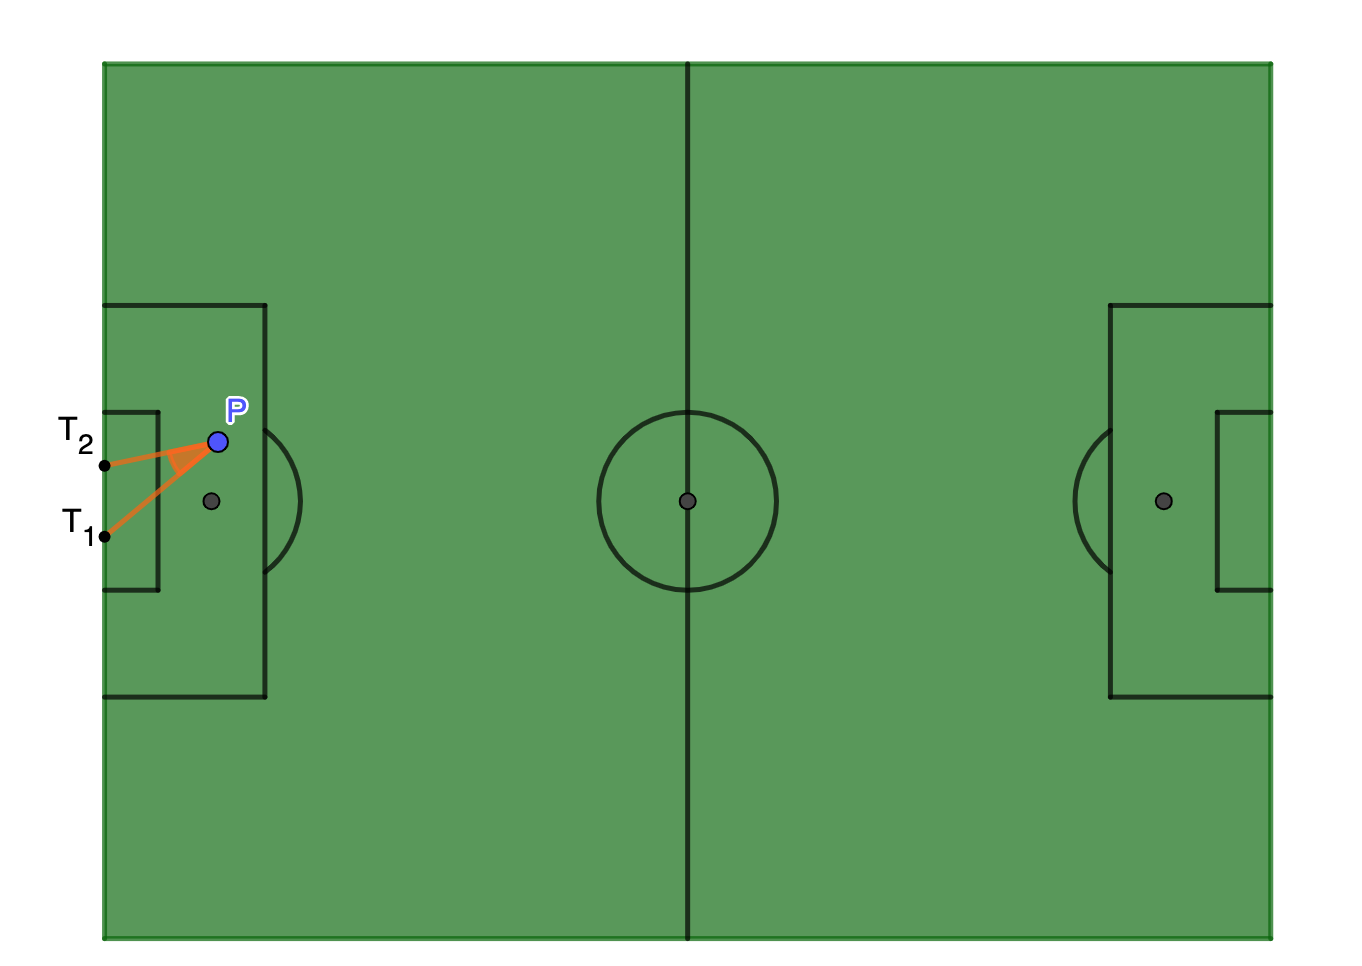
\includegraphics[scale=.4]{sec2_futebol1.png}
    \caption{Ângulo para um chute certeiro ao gol do jogador $P$.}
    \label{sec2_futebol1_fig}
\end{figure}



    \item{}
    Sempre que necessário, os valores numéricos sejam aproximados com 3 casas decimais.
\end{itemize}
\newpage

\paragraph{Parte I}

\begin{enumerate}
    \item{}
    Considere dois jogadores $A$ e $B$ posicionados dentro do campo de futebol, como na \Fref{sec2_futebol2_fig}. O jogador $A$ está sobre a quina da grande área e o jogador $B$ fora da grande área e próximo ao círculo central do campo. Analisando apenas visualmente a situação, na sua opinião, qual jogador possui o maior ângulo para um chute certeiro ao gol? Discuta com seu colega.
\begin{figure}[H]
    \centering
    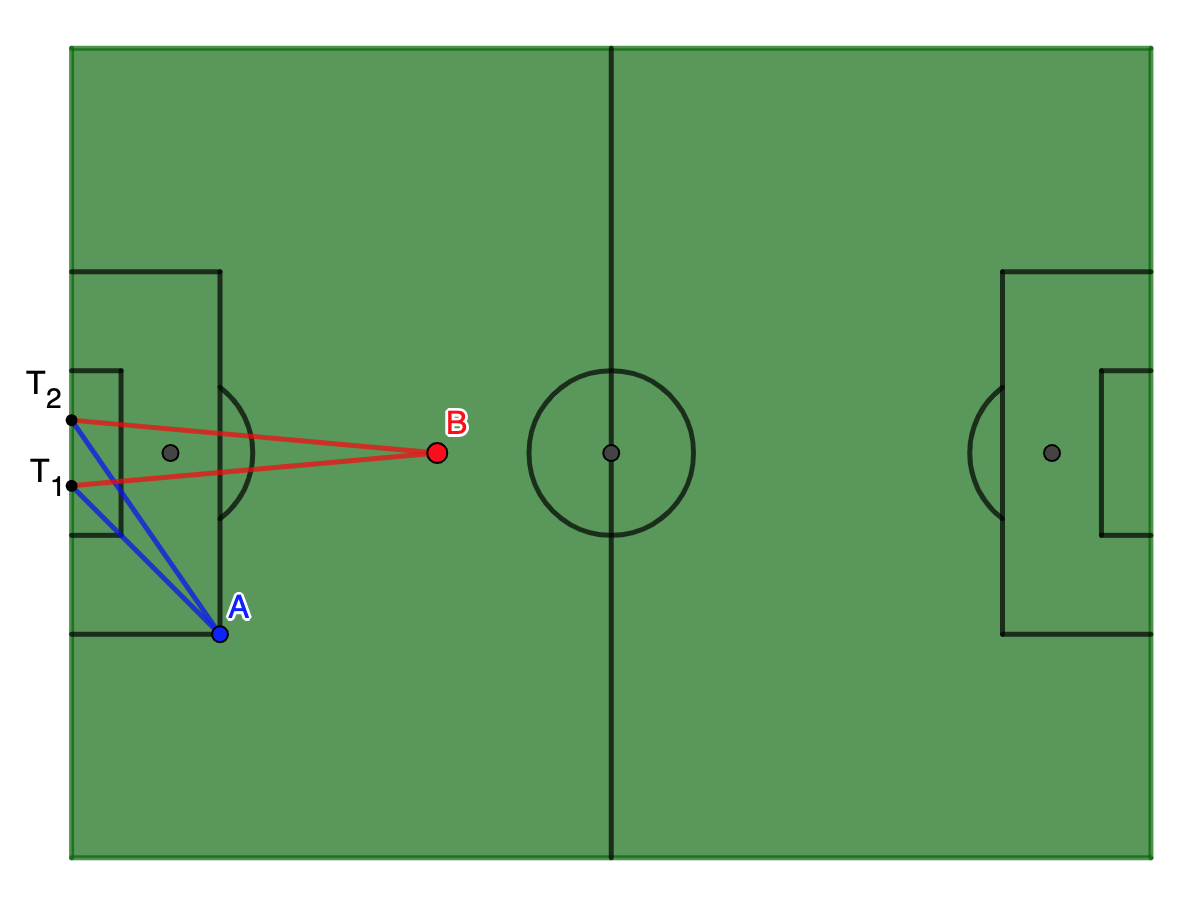
\includegraphics[scale=0.35]{sec2_futebol2.png}
    \caption{Jogadores $A$ e $B$ se preparando para um chute ao gol.}
    \label{sec2_futebol2_fig}
\end{figure}



    \item{}
    Considere $AT_1=23,33, AT_2=28,96$ e $BT_1=BT_2=40,82$. Utilizando seus conhecimentos geométricos e as medidas do campo de futebol disponíveis na \Fref{sec2_futebol4_fig}, tente confirmar sua resposta ao item anterior. Se você não tiver chegado a uma conclusão do item anterior, não se preocupe. Com os valores dados neste item, você terá uma nova oportunidade de buscar a resposta. Se for preciso, use a tabela trigonométrica presente no final do capítulo com aproximações dos valores de seno e cosseno de diversos ângulos para resolver a atividade.
\begin{figure}[H]
    \centering
    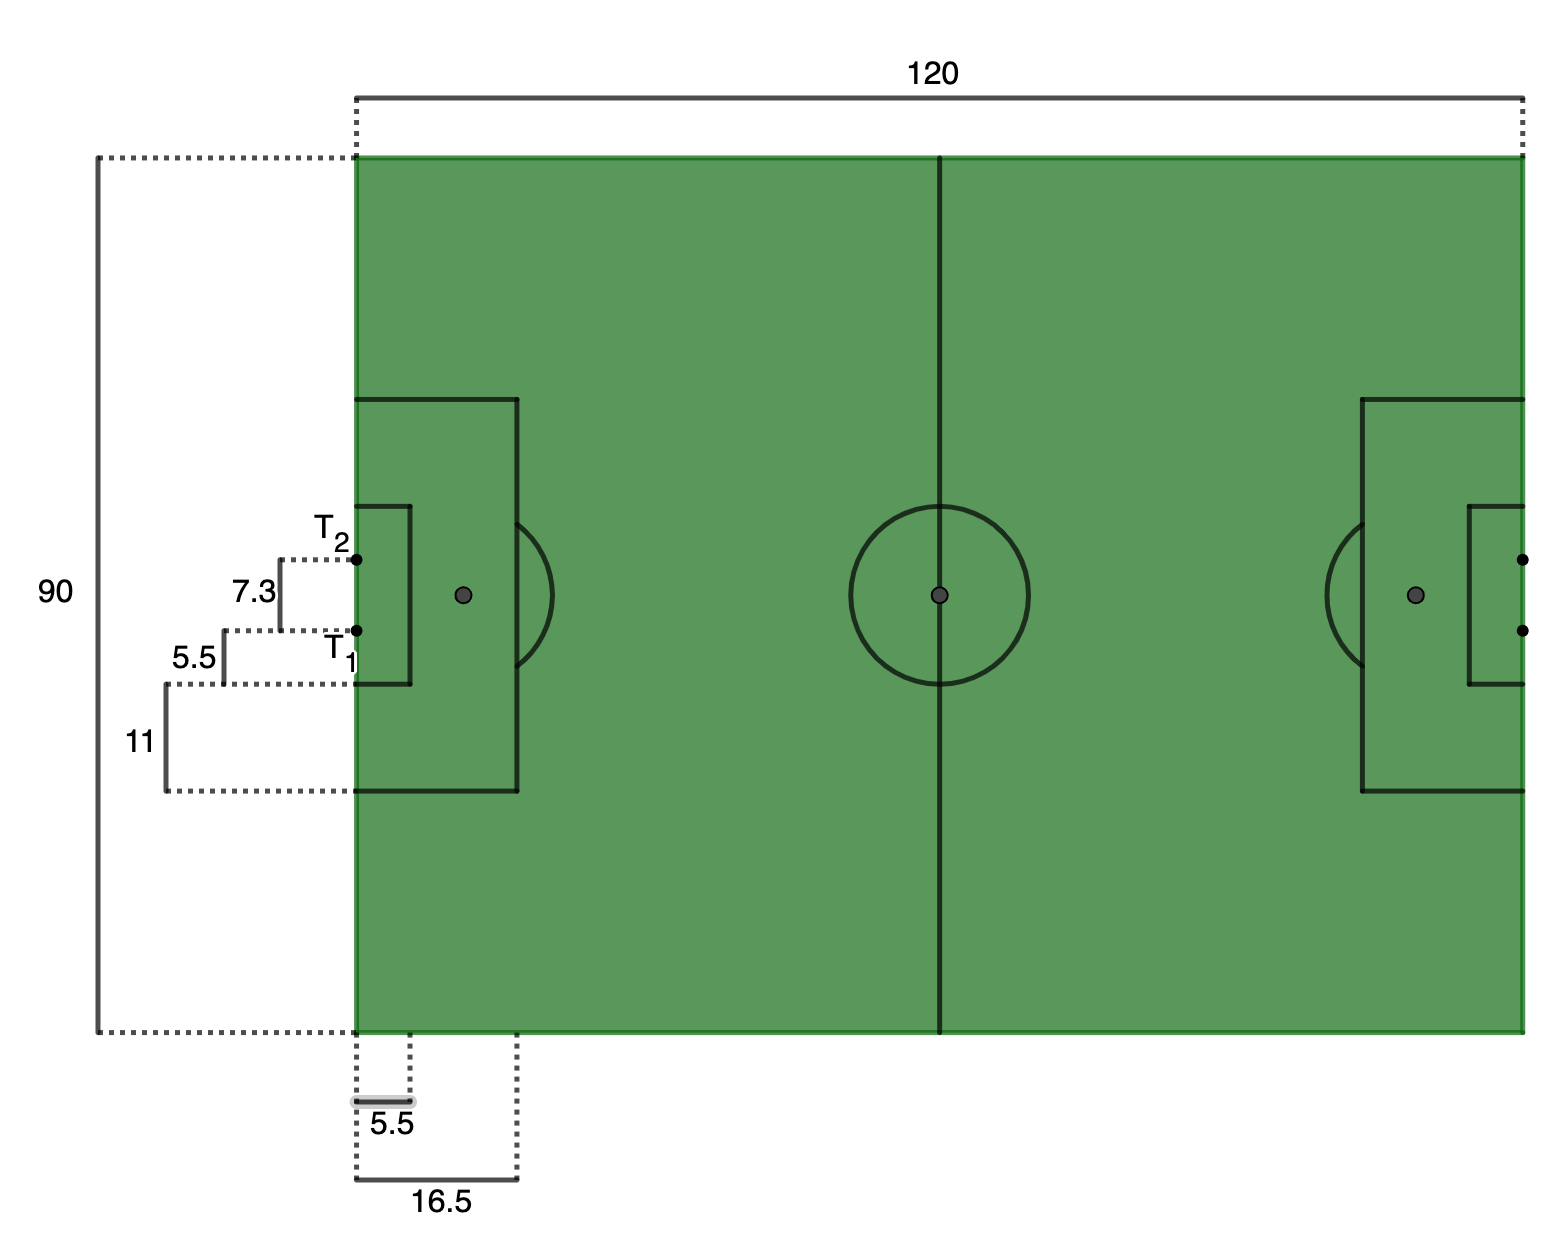
\includegraphics[scale=0.3]{sec2_futebol4.png}
    \caption{Medidas do campo de futebol do jogo.}
    \label{sec2_futebol4_fig}
\end{figure}

    
    \item{}
    Agora, o desenvolvedor de jogos precisa adicionar um novo jogador ao cenário anterior, o jogador $C$, como na \Fref{sec2_futebol3_fig}. Assim como fizemos anteriormente, analise a situação visualmente e decida se é possível apontar, dentre os jogadores $A, B$ e $C$, qual deles possui o maior ângulo para um chute certeiro ao gol. Discuta com seu colega.
\begin{figure}[H]
    \centering
    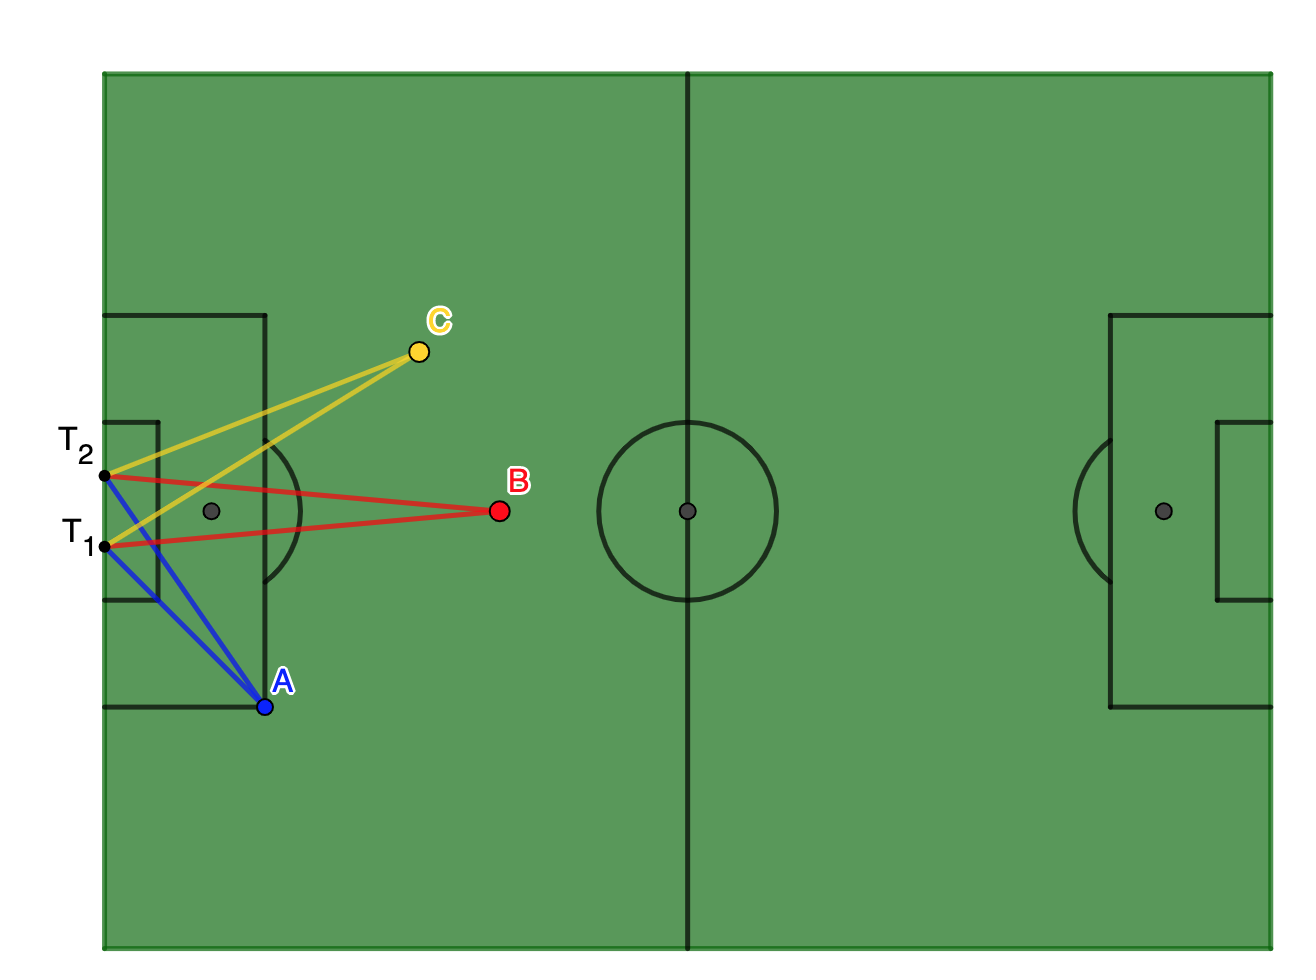
\includegraphics[scale=0.4]{sec2_futebol3.png}
    \caption{Jogadores $A, B$ e $C$.}
    \label{sec2_futebol3_fig}
\end{figure}



    \item{}
    Considere $CT_1=38,08$ e $CT_2=34,79$. Após utilizar seus conhecimentos geométricos e as medidas do campo de futebol disponíveis na \Fref{sec2_futebol4_fig}, você manteria sua resposta do item anterior?

    \item{}
    Apenas com os dados das distâncias dos jogadores às traves que delimitam o gol, o desenvolvedor de jogos poderá calcular todos os ângulos de chutes certeiros ao gol? Você teria alguma sugestão para ajudar esse desenvolvedor? Existe alguma informação que poderia ser adicionada à situação para auxiliar na solução do problema do desenvolvedor?
    
    Caso tenha acesso a Internet (inclusive de um celular), você pode interagir com jogadores dentro de um campo de futebol por meio do aplicativo GeoGebra disponível em: <https://www.geogebra.org/m/aezzjs3c>
    
\end{enumerate}

\newpage

\paragraph{Parte II} 

Agora, vamos utilizar os dados que foram usados na PARTE I desta atividade para responder aos itens seguintes.

\begin{enumerate}

    \item{}
    Sejam $a$ a distância entre os pés das traves, e $b$ e $c$ as distâncias entre a posição de um jogador qualquer dentro de campo e os pés das traves. Usando os dados na PARTE I desta atividade para os jogadores A, B e C, preencha a \Tref{sec2_tabfutebol1}.
\begin{table}[H]
\centering
\begin{tabular}{|c|c|c|c|}
\hline
\tcolor{Jogador} & $\tmat{\quad a \quad}$ & $\tmat{\quad b \quad}$ & $\tmat{\quad c \quad}$ \\ %
\hline                               
A & & &  \\
\hline
B & & & \\
\hline
C & & & \\
\hline
\end{tabular}
\caption{Dados dos jogadores $A, B$ e $C$.}
\label{sec2_tabfutebol1}
\end{table}

\item{}
Vamos agora inserir uma coluna na \Tref{sec2_tabfutebol1} para calcular o valor de 
$$\fra{b^2+c^2-a^2}{2bc}$$
para cada uma das posições dos jogadores, como pode ser visto na \Tref{sec2_tabfutebol2}.
\begin{table}[H]
\centering
\begin{tabular}{|c|c|c|c|e{3.1cm}|}
\hline
\tcolor{Jogador} & $\tmat{\quad a \quad}$ & $\tmat{\quad b \quad}$ & $\tmat{\quad c \quad}$ & \tcolor{$\quad  \dfrac{\bm{b^2+c^2-a^2}}{\bm{2bc}} \quad$} \tabularnewline
\hline                               
$A$ & & & & \tabularnewline
\hline
$B$ & & & & \tabularnewline
\hline
$C$ & & & & \tabularnewline
\hline
\end{tabular}
\caption{Dados dos jogadores $A, B$ e $C$.}
\label{sec2_tabfutebol2}
\end{table}

    \item{}
    Analisando a \Tref{sec2_tabfutebol2} preenchida com os dados pedidos, o que é possível concluir? Tente analisar a tabela lembrando da sua resposta para o item (d) da PARTE I desta atividade.
\end{enumerate}
\end{task}

\arrange{Lei dos Cossenos}
\label{org_leidoscossenos}

Nas atividades anteriores, repare que o teorema de Pitágoras e as razões trigonométricas dos ângulos dos chutes ao gol não puderam ser aplicados diretamente para solucionar os problemas. Isso se deve ao fato de os triângulos que modelam as situações estudadas não serem triângulos retângulos. Por isso, a partir destes triângulos, tivemos que criar triângulos retângulos para, então, fazer uso das razões trigonométricas. A partir daí, conseguimos resolver o problema.

Nessa seção, nosso objetivo é generalizar o que foi feito no caso particular da atividade anterior obtendo um teorema que pode ser utilizado em qualquer triângulo e que é chamado lei dos cossenos. Esse teorema responde à pergunta que fizemos no início da seção sobre existir uma relação entre os lados de um triângulo qualquer. Depois de sua apresentação e demonstração, refletiremos sobre a pergunta feita no início da seção.

Primeiramente, enunciaremos e demonstraremos a lei dos cossenos para triângulos acutângulos. Na verdade, mesmo sem saber, você já fez isso no caso particular da atividade do jogo de videogame, mas agora refaremos todos os passos da solução de tal atividade de uma maneira geral que vale para  triângulos acutângulos. Mais adiante, estenderemos esse resultado para triângulos retângulos e obtusângulos.

\begin{observationtitle}{Lei dos Cossenos - parte 1}
\leavevmode\phantomsection\label{sec2_leidoscossenos_parte1}
Seja $ABC$ um triângulo acutângulo, onde $a, b$ e $c$ são as medidas dos lados $BC, AC$ e $AB$, respectivamente, e $\alpha=\angle(C\hat{A}B)$ como na \Fref{sec2_leidoscossenos_enunciado1}. Então,
\begin{equation}
    a^2=b^2+c^2-2bc\cos\alpha. \label{sec2_leidoscossenos_acut_eq}
\end{equation}
\begin{figure}[H]
    \centering
    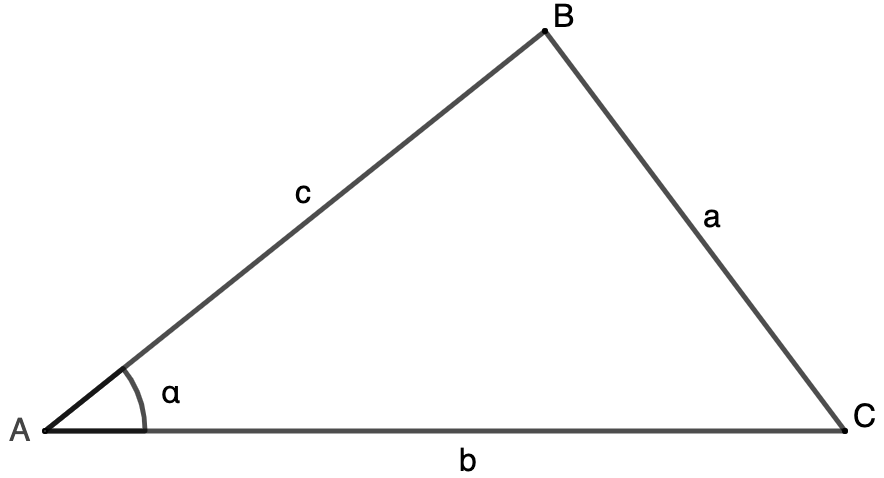
\includegraphics[scale=0.4]{sec2_leidoscossenos_enunciado.png}
    \caption{O triângulo $ABC$ é acutângulo com ângulo interno $\alpha$.}
    \label{sec2_leidoscossenos_enunciado1}
\end{figure}
\end{observationtitle}


\paragraph{Demonstração da Lei dos Cossenos - parte 1}
\phantomsection\label{sec2_leidoscossenos_demo}
Vamos, então, considerar o triângulo acutângulo $ABC$, como na \Fref{sec2_leidoscossenos_enunciado1}.

Seja $BD$ a altura do triângulo $ABC$ traçada a partir do vértice $B$ e $h$ a medida de sua altura. Para facilitar os cálculos, vamos chamar de $u$ e $v$ as medidas dos segmentos $AD$ e $DC$, respectivamente. Neste caso, $b=u+v$. Veja a \Fref{sec2_leidoscossenos_acut_demo1_fig}.

\begin{figure}[H]
    \centering
    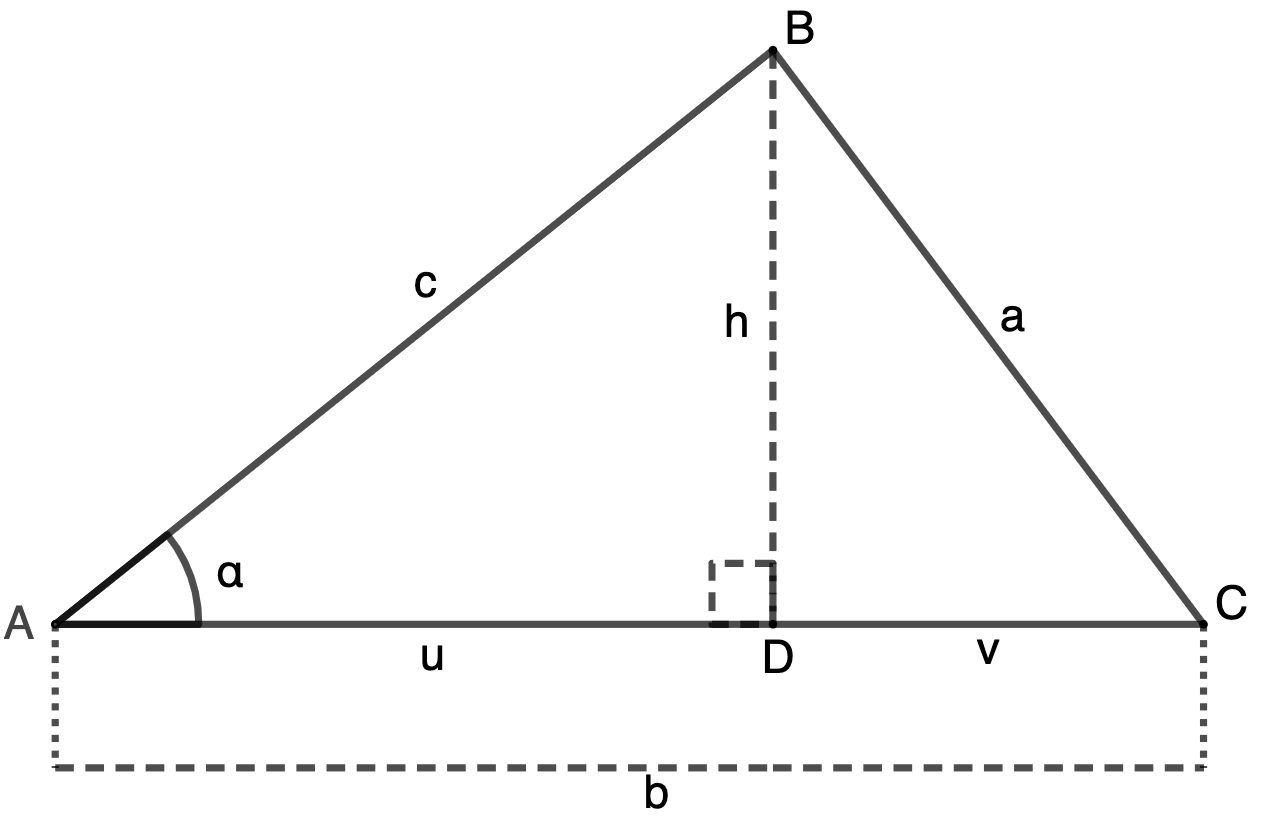
\includegraphics[scale=0.7]{sec2_leisdoscossenos_acut_demo1.png}
    \caption{Triângulo $ABC$ com altura $BD$.}
    \label{sec2_leidoscossenos_acut_demo1_fig}
\end{figure}

Repare que $ADB$ é um triângulo retângulo em $D$. Usando as razões trigonométricas estudadas na seção anterior neste triângulo, temos:
\begin{eqnarray}{}
 \sen\alpha = \fra{h}{c} & \iff h=c\sen\alpha, \label{sec2_leidoscossenos_demo_eq3}\\ 
 \cos\alpha = \fra{u}{c} & \iff u=c\cos\alpha. \label{sec2_leidoscossenos_demo_eq4}
\end{eqnarray}

Além disso, $BDC$ é um triângulo retângulo em $D$, então, o teorema de Pitágoras nos garante que:
\begin{equation}
    a^2=h^2+v^2. \label{sec2_leidoscossenos_demo_eq5}
\end{equation}

Como $v=b-u$, a equação \eqref{sec2_leidoscossenos_demo_eq5} pode ser reescrita da seguinte forma:
\begin{equation}
    a^2=h^2+(b-u)^2. \label{sec2_leidoscossenos_demo_eq6}
\end{equation}

Substituindo as equações \eqref{sec2_leidoscossenos_demo_eq3} e \eqref{sec2_leidoscossenos_demo_eq4} na equação \eqref{sec2_leidoscossenos_demo_eq6}, obtemos:
$$a^2=(c\sen\alpha)^2+(b-c\cos\alpha)^2,$$
ou seja,
\begin{equation}\label{sec2_leidoscossenos_demo_eq7}
    a^2=c^2\sen^2\alpha+b^2-2bc\cos\alpha+c^2\cos^2\alpha = c^2(\sen^2\alpha+\cos^2\alpha)+b^2-2bc\cos\alpha.
\end{equation}
Pela relação fundamental, a equação \eqref{sec2_leidoscossenos_demo_eq7} pode ser reescrita:
$$a^2=b^2+c^2-2bc\cos\alpha,$$
\noindent mostrando que \eqref{sec2_leidoscossenos_acut_eq} vale nesse caso.


\begin{reflection}
Compare a equação fornecida pela lei dos cossenos e a quarta coluna da \Tref{sec2_tabfutebol2}. Faz sentido os valores aproximados da quarta coluna serem tão próximos?
\end{reflection}

Este resultado é o primeiro passo na direção de respondermos à pergunta do início da seção sobre a existência de um resultado que relacione os lados de um triângulo qualquer.
%
No caso do triângulo acutângulo, agora, já sabemos que essa relação existe, mas ela também utiliza o cosseno de um ângulo interno do triângulo, que neste caso é sempre agudo.
%
Será que é possível encontrar um resultado semelhante a esse para triângulos retângulos e obtusângulos? 

Caso trabalhemos com triângulos retângulos e obtusângulos, seus ângulos internos podem ser retos ou obtusos, além de agudos. 
%
Porém, caso o ângulo seja reto ou obtuso, sabemos calcular seu cosseno? 
%
A resposta é: com o que aprendemos até aqui não. 
%
Sendo assim, vamos ampliar a definição de cosseno de um ângulo agudo para um ângulo qualquer entre $0^\circ$ e $180^\circ$, antes de procedermos com o estudo da lei dos cossenos. 

Já sabemos calcular o cosseno de um ângulo agudo com o que aprendemos na seção anterior, a definição a seguir contemplará agora todos os ângulos entre $0^\circ$ e $180^\circ$. Vejamos.

Definimos:
\begin{itemize}[topsep=0pt, itemsep=0pt]
\item $\cos(0^\circ)=1$;
\item $\cos(90^\circ)=0$;
\item $\cos(180^\circ)=-1$;
\item para um ângulo obtuso $\alpha$, $\cos\alpha=-\cos(180^\circ-\alpha).$
\end{itemize}

Nesta definição, utilizamos o cosseno de $180^\circ-\alpha$ para definir o cosseno de $\alpha$. Note que se $\alpha$ é um ângulo obtuso, então $180^\circ-\alpha$ é um ângulo agudo e portanto, sabemos calcular seu cosseno com o conteúdo que aprendemos até aqui.

Por agora, basta que tenhamos a definição anterior em mente para continuarmos nosso estudo de Trigonometria. Se você quiser saber um pouco mais sobre essa definição, veja o \textit{Para saber+ Explorando a definição de senos e cossenos}. E ainda, no capítulo que trata as funções trigonométricas, você terá a oportunidade de trabalhar mais profundamente com cossenos (e senos também) de um ângulo qualquer, indo além do que estamos vendo aqui.

\begin{observation}
Já sabemos que o cosseno de um ângulo agudo $\alpha$ assume apenas valores positivos e menores que $1$, então, de acordo com a definição acima,  
$$\text{se }0^\circ \leq\alpha \leq180^\circ, \text{então} -1\leq\cos\alpha\leq 1.$$
\end{observation}

Agora, de posse dessas informações, vamos enunciar e demonstrar a lei dos cossenos para qualquer triângulo retângulo e obtusângulo. 

\begin{observationtitle}{Lei dos Cossenos - Parte 2}
\leavevmode\phantomsection\label{sec2_leidoscossenos_parte2}
Seja $ABC$ um triângulo retângulo em $A$ ou obtusângulo, onde $a, b$ e $c$ são as medidas dos lados $BC, AC$ e $AB$, respectivamente, e $\alpha=\angle(C\hat{A}B)$ como na \Fref{sec2_leidoscossenos_enunciado2}. Então,
\begin{equation}\label{sec2_leidoscossenos_eq2}
    a^2=b^2+c^2-2bc\cos\alpha.
\end{equation}
\begin{figure}[H]
    \centering
    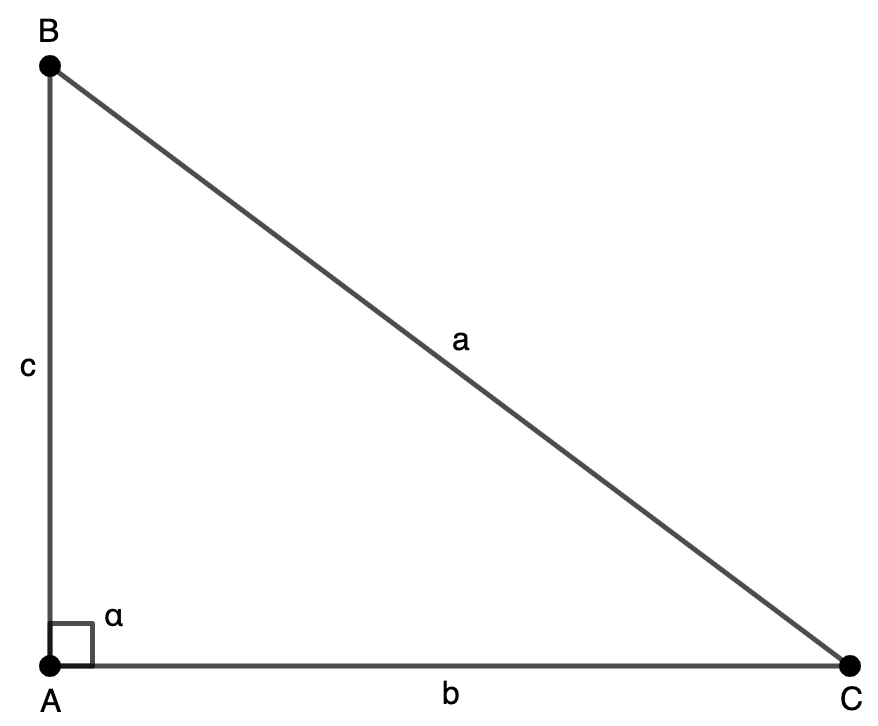
\includegraphics[height=.115\textheight]{sec2_leidoscossenos_enunciado_trigret.png}
    %\hspace{1.5cm}
    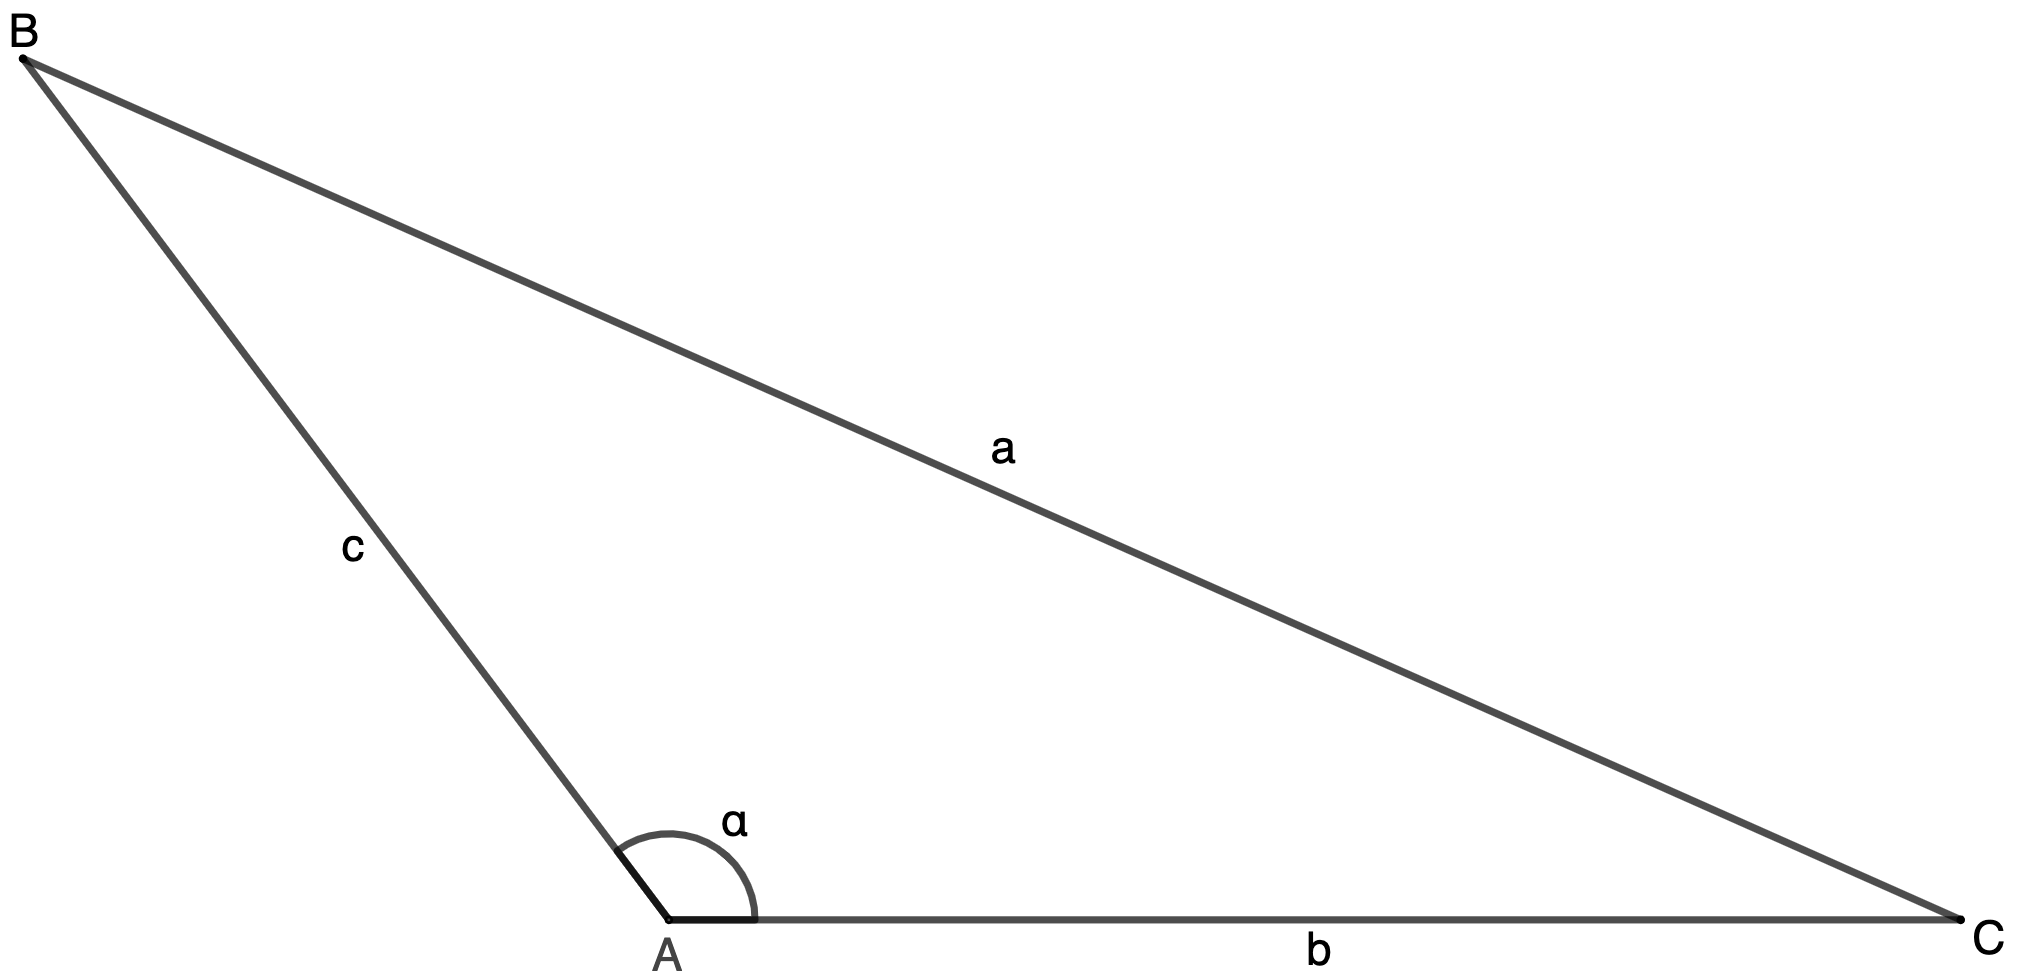
\includegraphics[height=.115\textheight]{sec2_leidoscossenos_enunciado_trigobt1.png}
    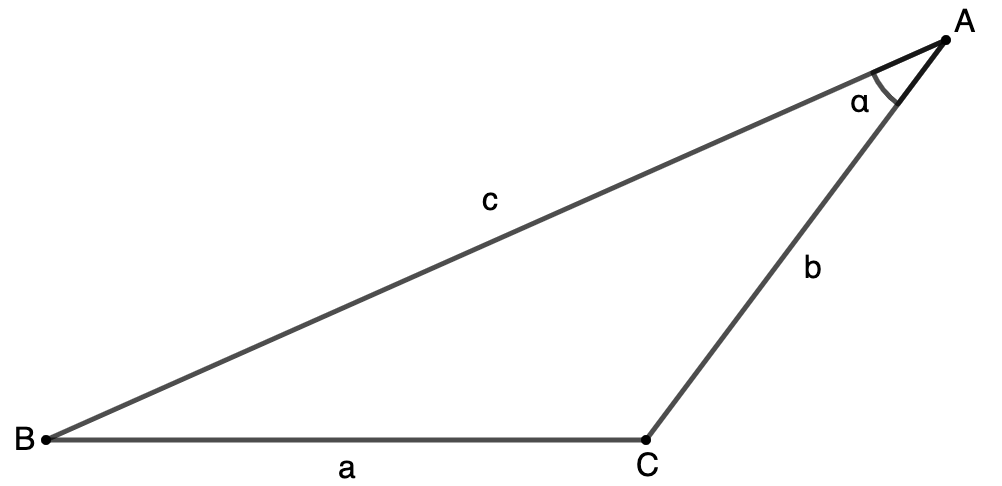
\includegraphics[height=.115\textheight]{sec2_leidoscossenos_enunciado_trigobt2.png}
    \caption{O triângulo $ABC$ da esquerda é retângulo em $A$, enquanto o central é obtusângulo com ângulo $\alpha$ obtuso e o da direita é obtusângulo com ângulo $\alpha$ agudo.}
    \label{sec2_leidoscossenos_enunciado2}
\end{figure}
\end{observationtitle}

\paragraph{Demonstração da Lei dos Cossenos}
\phantomsection\label{sec2_leidoscossenos_demo2}

Nesta demonstração, precisamos considerar que $ABC$ pode ser um triângulo retângulo em $A$ ou obtusângulo, como mostra a \Fref{sec2_leidoscossenos_enunciado2}. Dividiremos, então, essa demonstração em duas partes. Na primeira parte, trabalharemos apenas com um triângulo retângulo e na segunda, com um triângulo obtusângulo que poderá ter $\alpha$ agudo ou obtuso.

Primeira parte: $ABC$ é retângulo em $A$.

Estamos considerando, nesta parte, que $\alpha=90^\circ$. Veja a \Fref{sec2_leidoscossenos_fig_demoret1}.

\begin{figure}[H]
    \centering
    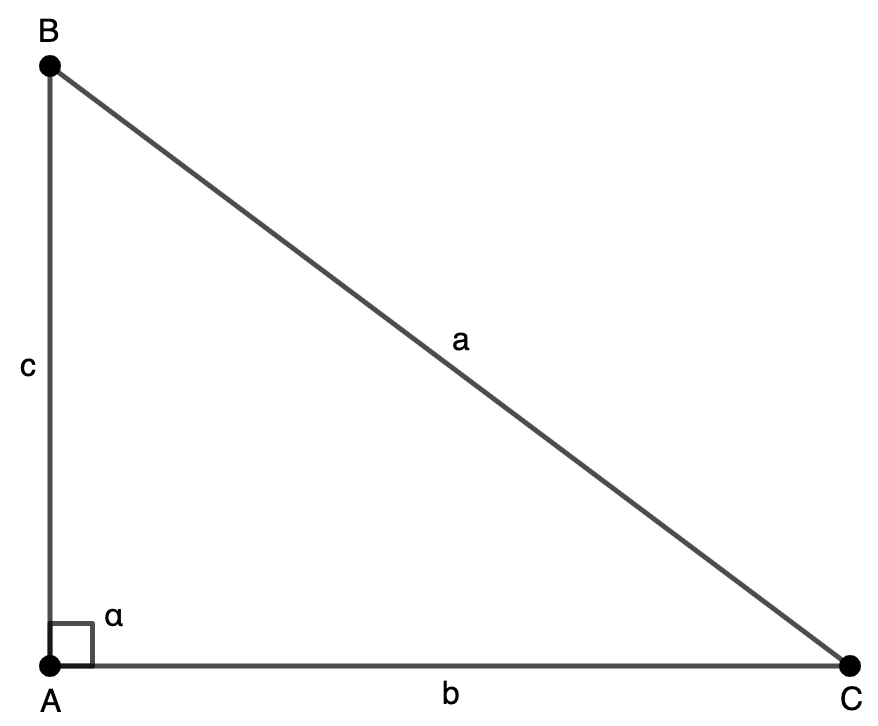
\includegraphics[scale=0.3]{sec2_leidoscossenos_enunciado_trigret.png}
     \caption{O triângulo $ABC$ é retângulo em $A$.}
    \label{sec2_leidoscossenos_fig_demoret1}
\end{figure}

Pela definição anterior, $\cos \alpha = \cos 90^\circ=0$, então 
\begin{equation}\label{sec2_leidoscossenos_demoret1}
b^2+c^2-2bc\cos\alpha= b^2+c^2-2bc \cdot 0 = b^2+c^2.
\end{equation}

Por outro lado, o triângulo $ABC$ é retângulo em $A$ e portanto, pelo teorema de Pitágoras sabemos que
\begin{equation}\label{sec2_leidoscossenos_demoret2}
a^2=b^2+c^2.
\end{equation}

\no Unindo as equações \eqref{sec2_leidoscossenos_demoret1} e \eqref{sec2_leidoscossenos_demoret2}, concluímos que
$$a^2=b^2+c^2-2bc\cos\alpha,$$
mostrando assim que \eqref{sec2_leidoscossenos_eq2} vale nesse caso.

\vspace{0.5cm}

Segunda parte: $ABC$ é obtusângulo.

Precisamos, nesta parte, considerar que o ângulo $\alpha$ pode ser obtuso ou agudo. A seguir, trabalharemos com cada uma das possibilidades.

Consideremos primeiramente que $\alpha$ é obtuso. Veja a \Fref{sec2_leidoscossenos_fig_demo_obtusangulo_obtuso1}.

\begin{figure}[H]
    \centering
    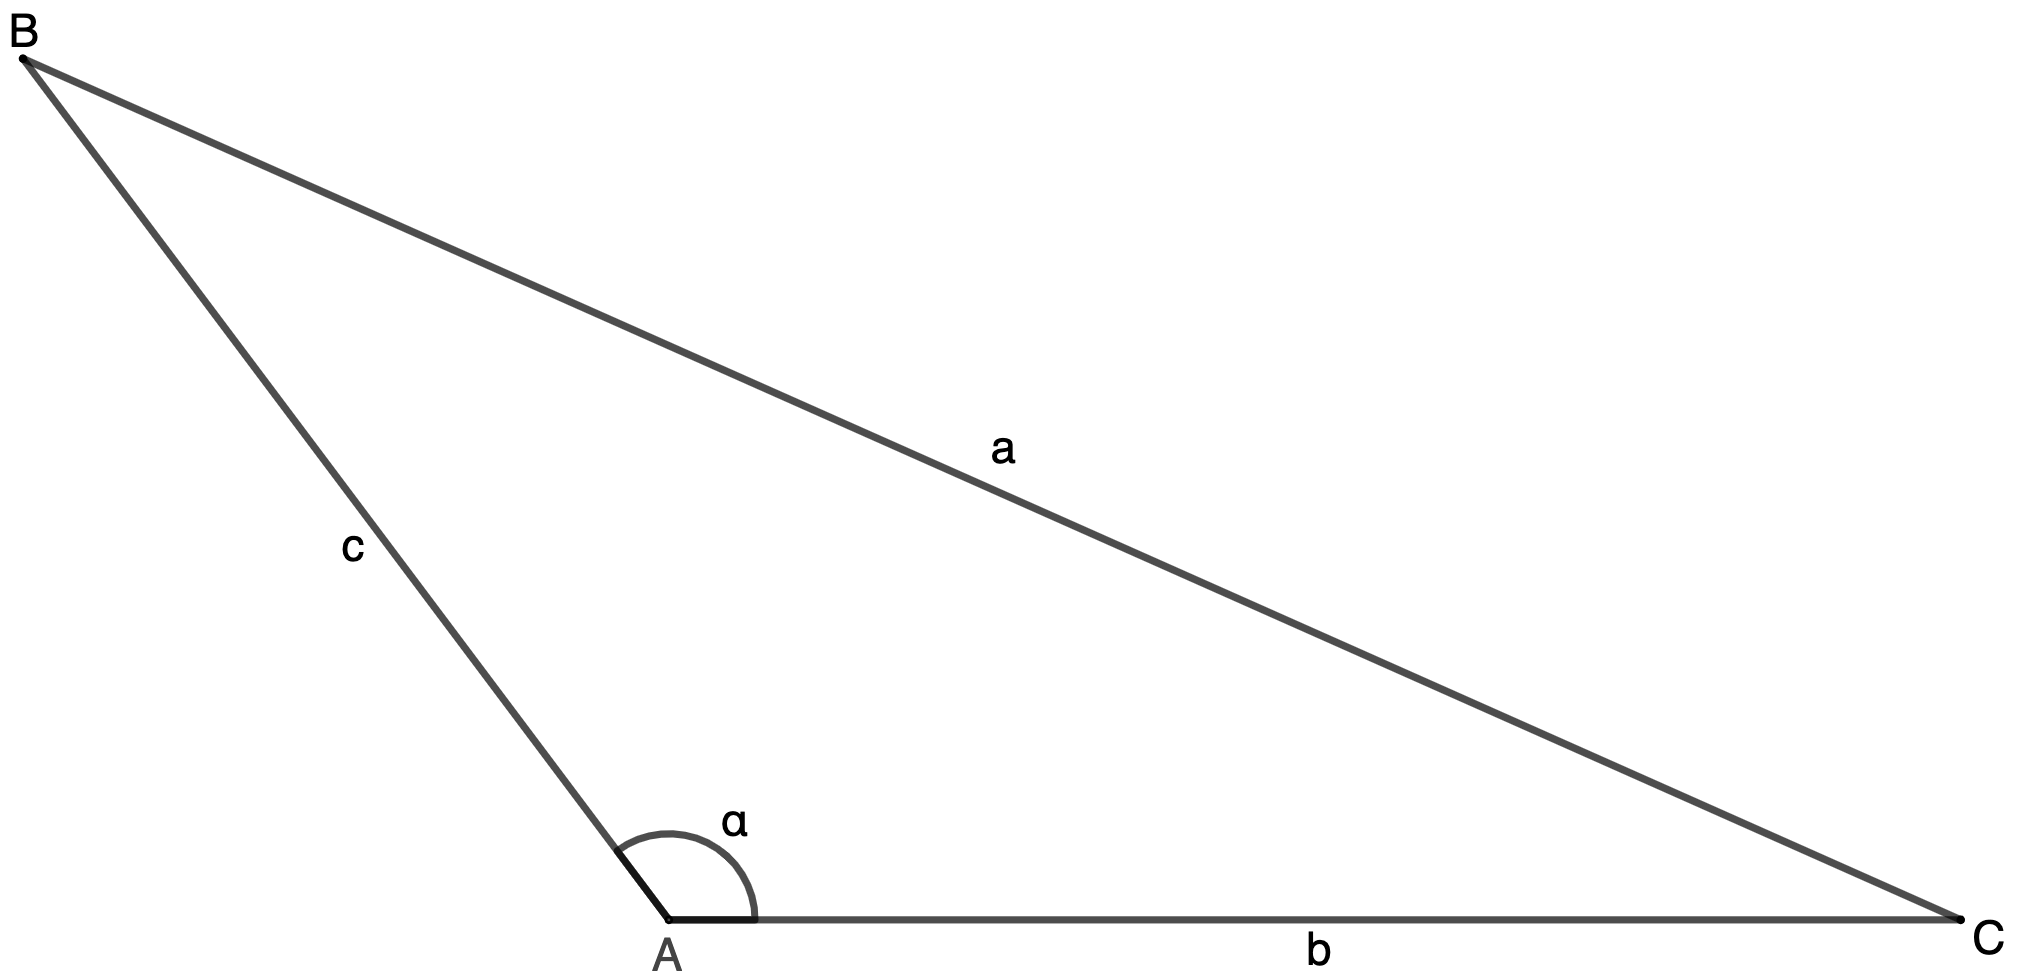
\includegraphics[scale=0.7]{sec2_leidoscossenos_enunciado_trigobt1.png}
    \caption{Triângulo $ABC$ onde $\alpha$ é um ângulo obtuso.}
    \label{sec2_leidoscossenos_fig_demo_obtusangulo_obtuso1}
\end{figure}

Seja, então, $BD$ a altura do triângulo $ABC$ traçada a partir do vértice $B$, como podemos ver na \Fref{sec2_leidoscossenos_fig_demo_obtusangulo_obtuso2}. Denotemos por $h$ e $u$ as medidas da altura $BD$ e do segmento $AD$, respectivamente.

\begin{figure}[H]
    \centering
    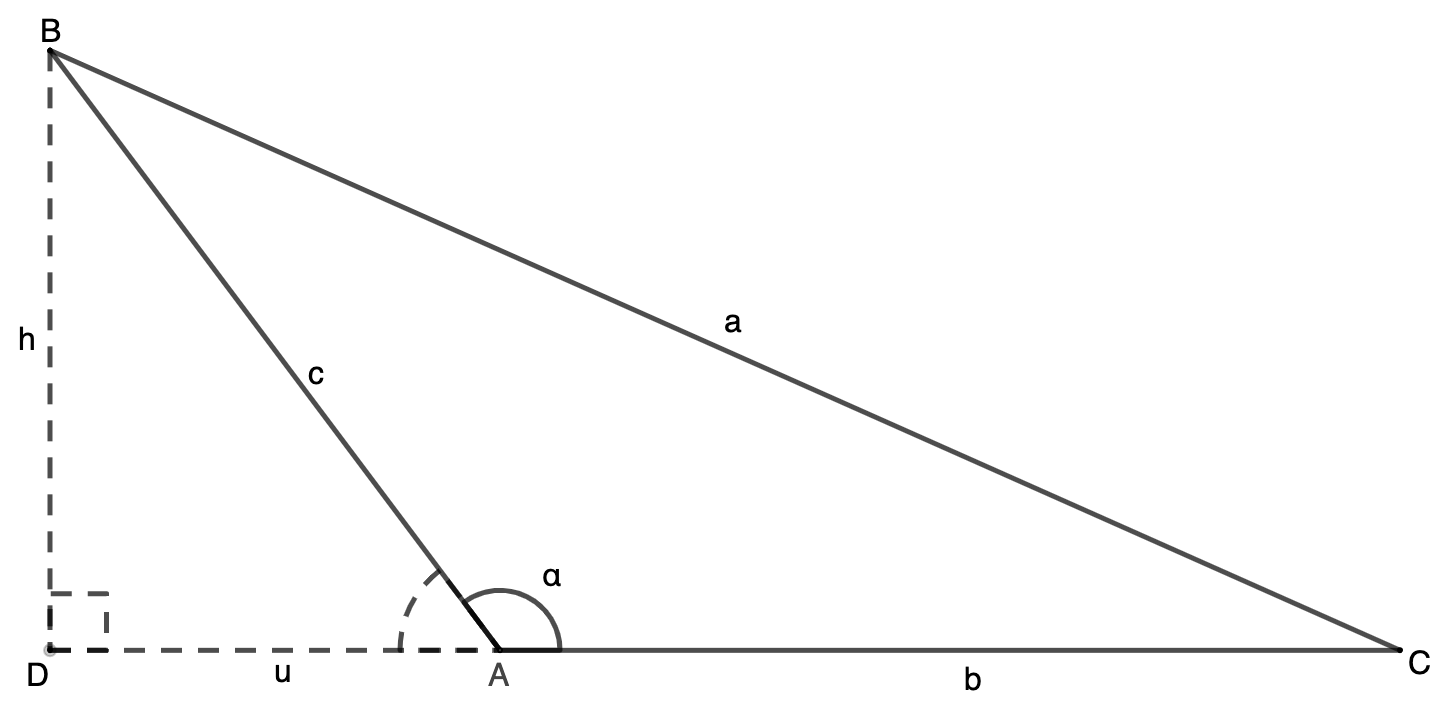
\includegraphics[scale=0.3]{sec2_leidoscossenos_demoobtuso.png}
    \caption{Triângulo $ABC$ onde $\alpha$ é um ângulo obtuso.}
    \label{sec2_leidoscossenos_fig_demo_obtusangulo_obtuso2}
\end{figure}

Repare que $ADB$ é um triângulo retângulo em $D$. Usando as razões trigonométricas estudadas na seção anterior, temos:
\begin{eqnarray}{}
 \sen (180^\circ-\alpha) = \fra{h}{c} & \iff h=c\sen (180^\circ-\alpha), \label{sec2_leidoscossenos_demo8}\\ 
 \cos (180^\circ-\alpha) = \fra{u}{c} & \iff u=c\cos (180^\circ-\alpha). \label{sec2_leidoscossenos_demo9}
\end{eqnarray}

E ainda, podemos notar que $BDC$ é também um triângulo retângulo em $D$. Assim, aplicando o teorema de Pitágoras neste triângulo obtemos:
\begin{equation}
    a^2=h^2+(b+u)^2. \label{sec2_leidoscossenos_demo10}
\end{equation}

Substituindo as equações \eqref{sec2_leidoscossenos_demo8} e \eqref{sec2_leidoscossenos_demo9} em \eqref{sec2_leidoscossenos_demo10}, obtemos:
$$a^2=(c\sen (180^\circ-\alpha))^2+(b+c\cos (180^\circ-\alpha))^2,$$
ou seja,
$$\begin{array}{ccc}
    a^2 & = &  c^2\sen^2 (180^\circ-\alpha)+b^2+2bc\cos (180^\circ-\alpha)+c^2\cos^2 (180^\circ-\alpha)\\
    & = & c^2(\sen^2 (180^\circ-\alpha)+\cos^2 (180^\circ-\alpha))+b^2+2bc\cos (180^\circ-\alpha).
\end{array}$$
Usando a relação fundamental, concluímos que:
\begin{equation}
    a^2=b^2+c^2+2bc\cos (180^\circ-\alpha).\label{sec2_leidoscossenos_demo11}
\end{equation}

Pela definição anterior, temos que $\cos(180^\circ-\alpha)=-\cos\alpha$, portanto, 
$$a^2=b^2+c^2-2bc\cos\alpha,$$
mostrando assim que \eqref{sec2_leidoscossenos_eq2} vale neste caso.

Consideremos agora que $\alpha$ é agudo. Veja a \Fref{sec2_leidoscossenos_fig_demo_obtusangulo_agudo1}.

\begin{figure}[H]
    \centering
    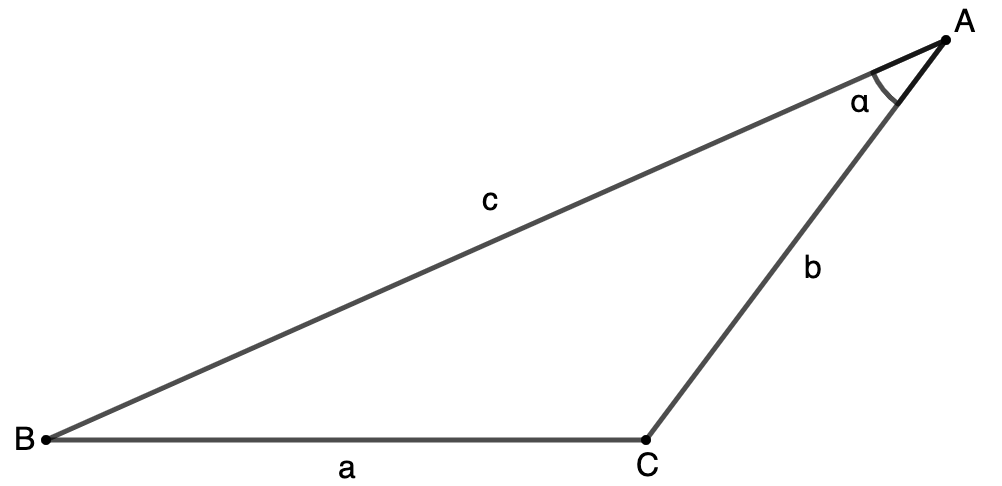
\includegraphics[scale=0.4]{sec2_leidoscossenos_enunciado_trigobt2.png}
    \caption{Triângulo $ABC$ onde $\alpha$ é um ângulo agudo.}
    \label{sec2_leidoscossenos_fig_demo_obtusangulo_agudo1}
\end{figure}

Considere $CD$ a altura do triângulo $ABC$ traçada a partir de $C$, como podemos ver na \Fref{sec2_leidoscossenos_fig_demo_obtusangulo_agudo2}. Chamaremos de $u, v$ e $h$ as medidas dos segmentos $AD, BD$ e $CD$, respectivamente.

\begin{figure}[H]
    \centering
    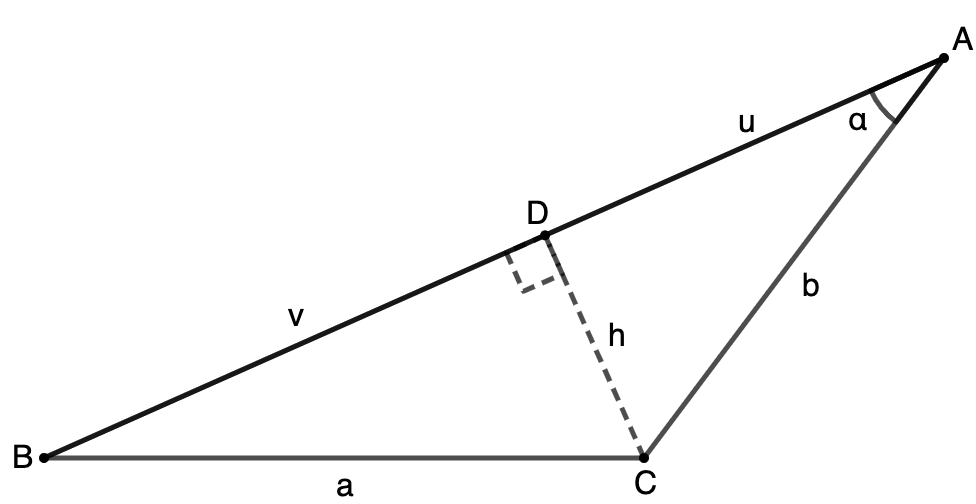
\includegraphics[scale=0.4]{sec2_leidoscossenos_demo_obtusangulo_agudo.png}
    \caption{Triângulo $ABC$ onde $\alpha$ é um ângulo agudo.}
    \label{sec2_leidoscossenos_fig_demo_obtusangulo_agudo2}
\end{figure}

Como $ACD$ é um triângulo retângulo em $D$, então 
\begin{equation}
    \cos\alpha=\frac{u}{b}.\label{sec2_leidoscossenos_demo12}
\end{equation}

Além disso, pelo teorema de Pitágoras, temos
 \begin{equation} 
    b^2=u^2+h^2. \label{sec2_leidoscossenos_demo13}
\end{equation}

Como $CDB$ também é um triângulo retângulo, então novamente pelo teorema de Pitágoras, temos
\begin{equation}
    a^2=v^2+h^2. \label{sec2_leidoscossenos_demo14}
\end{equation}

Da equação \eqref{sec2_leidoscossenos_demo13} temos que $h^2=b^2-u^2$. Substituindo em \eqref{sec2_leidoscossenos_demo14}, encontramos

\begin{eqnarray}{}
   a^2 & = & v^2+b^2-u^2 \nonumber\\
       & = & b^2+(v^2-u^2) \nonumber \\
       & = & b^2+(v+u)(v-u) \nonumber\\
       & = & b^2+c(v-u).\label{sec2_leidoscossenos_demo15}
\end{eqnarray}

Como $u+v=c \iff v=c-u$, por \eqref{sec2_leidoscossenos_demo12} temos que
\begin{equation}
    v-u=(c-u)-u=c-2u= c-2b\cos\alpha. \label{sec2_leidoscossenos_demo16}
\end{equation}

Substituindo \eqref{sec2_leidoscossenos_demo16} em \eqref{sec2_leidoscossenos_demo15} encontramos
$$a^2=b^2+c^2-2bc\cos\alpha,$$
mostrando que a equação \eqref{sec2_leidoscossenos_eq2} vale também para este caso.\hspace{4.5cm}$\square$


Após estudar a parte 1 e a parte 2 da lei dos cossenos, concluímos que, dado um triângulo qualquer $ABC$, onde $a, b$ e $c$ são as medidas dos lados $BC, AC$ e $AB$, respectivamente, e $\alpha=\angle(C\hat{A}B)$, vale a seguinte relação:
$$a^2=b^2+c^2-2bc\cos\alpha.$$

Você se lembra dos questionamentos que fizemos anteriormente sobre a existência de uma relação entre os lados em um triângulo qualquer? Somente agora, com os resultados da parte 1 e da parte 2 do teorema demonstrados, temos a possibilidade de responder ao que foi perguntado com convicção: sim, existe uma relação entre lados de um triângulo qualquer (chamada lei dos cossenos), mas diferentemente do teorema de Pitágoras, ela também envolve algum dos ângulos do triângulo. 

A lei dos cossenos recai sobre o teorema de Pitágoras caso $\alpha=90^\circ$, ou seja, se $ABC$ é um triângulo retângulo. Sendo assim, o teorema de Pitágoras pode ser visto como um caso particular da lei dos cossenos.

Vejamos a seguir um exemplo que busca encontrar a medida de um lado de um triângulo, dados um de seus ângulos e a medida dos outros dois lados.
\clearmargin
\def\currentcolor{session2}
\begin{objectives}{Estudando as câmeras de segurança de um estacionamento}
{
Aplicar a lei dos cossenos em um problema contextualizado. 
}{1}{1}
\end{objectives}
\begin{sugestions}{Estudando as câmeras de segurança de um estacionamento}
{
Nesta atividade serão utilizados os seguintes dados, que poderão ser acessados pelos estudantes na tabela trigonométrica do fim do capítulo: $\cos (55^\circ)=0,57$ e $\cos(125^\circ)=-0,57$. 

\textbf{Organização da turma}: em duplas.

\textbf{Conceitos abordados}: lei dos cossenos.

Dificuldades previstas: esta será a primeira vez, após a apresentação da lei dos cossenos, que os estudantes precisarão modelar um problema por um triângulo não retângulo e usar a lei para resolvê-lo. Como eles estarão diante de algo novo, é possível que ainda se sintam despreparados para resolver a questão e tenham dificuldade até mesmo para começar a solução. Caso essa seja a realidade dos estudantes, é importante que o professor auxilie os estudantes com uma interpretação correta da situação e também o uso adequado da lei dos cossenos. É muito comum o estudante não perceber que do lado esquerdo da equação dada pela lei dos cossenos está a medida ao quadrado do lado oposto ao ângulo considerado do lado direita da equação. Sendo assim, é preciso que o professor enfatize a correta interpretação da fórmula, de acordo com os dados do problema dado.
}{1}{1}1
\end{sugestions}
\begin{answer}{Estudando as câmeras de segurança de um estacionamento}
{
\begin{enumerate}
\item{} 
    A \Fref{sec2_resatestacionamento1} mostra o esboço da situação.
    \begin{figure}[H]
        \centering
        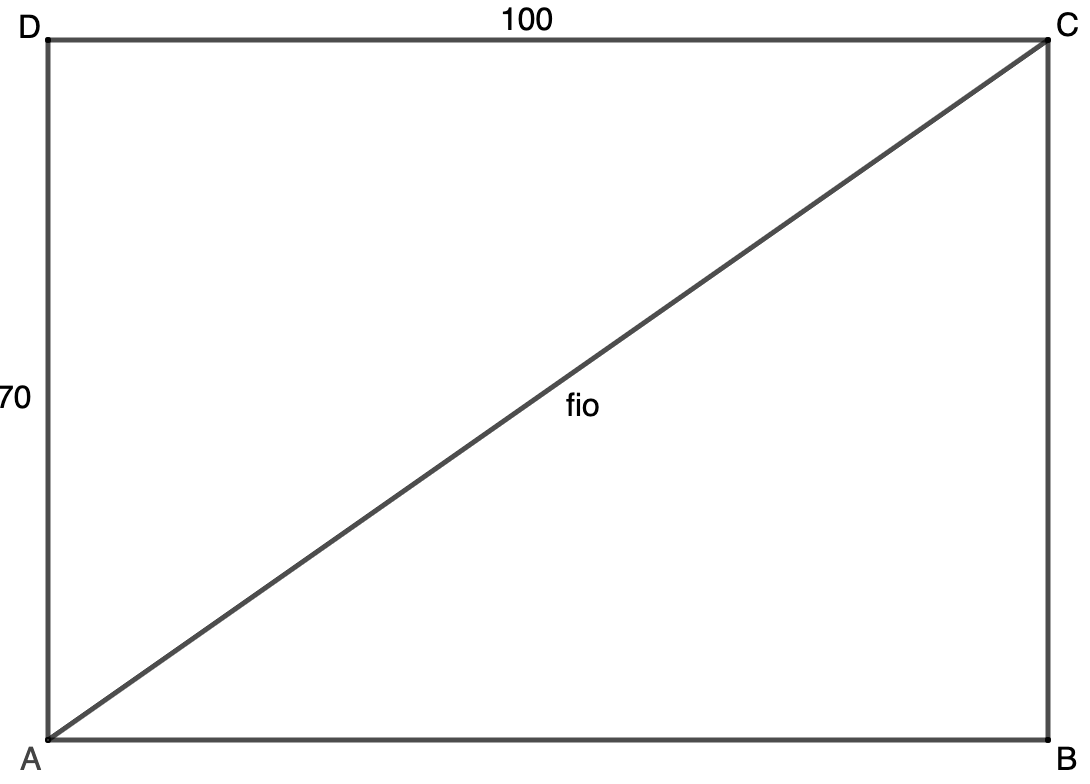
\includegraphics[scale=0.25]{sec2_atestacionamento1.png}
        \caption{Estacionamento em forma de retângulo $ABCD$.}
        \label{sec2_resatestacionamento1}
    \end{figure}
\end{enumerate}
}{1}
\end{answer}

\begin{answer}{Estudando as câmeras de segurança de um estacionamento}
{
\setcounter{enumi}{1}
\begin{enumerate}
\item Como o estacionamento é modelado por um retângulo onde conhecemos seus lados e o fio que será medido é a diagonal desse retângulo, é possível calcular o que é pedido utilizando o teorema de Pitágoras. 
    
    Nesse caso, $ABC$ é um triângulo retângulo em $B$. Assim, pelo teorema de Pitágoras obtemos 
    $$AC^2=100^2+70^2 \iff AC=10\sqrt{149}\text{m}$$
    que é o comprimento procurado do fio.

    \item{}
    A \Fref{sec2_resatestacionamento2} mostra o esboço da nova situação.
    \begin{figure}[H]
        \centering
        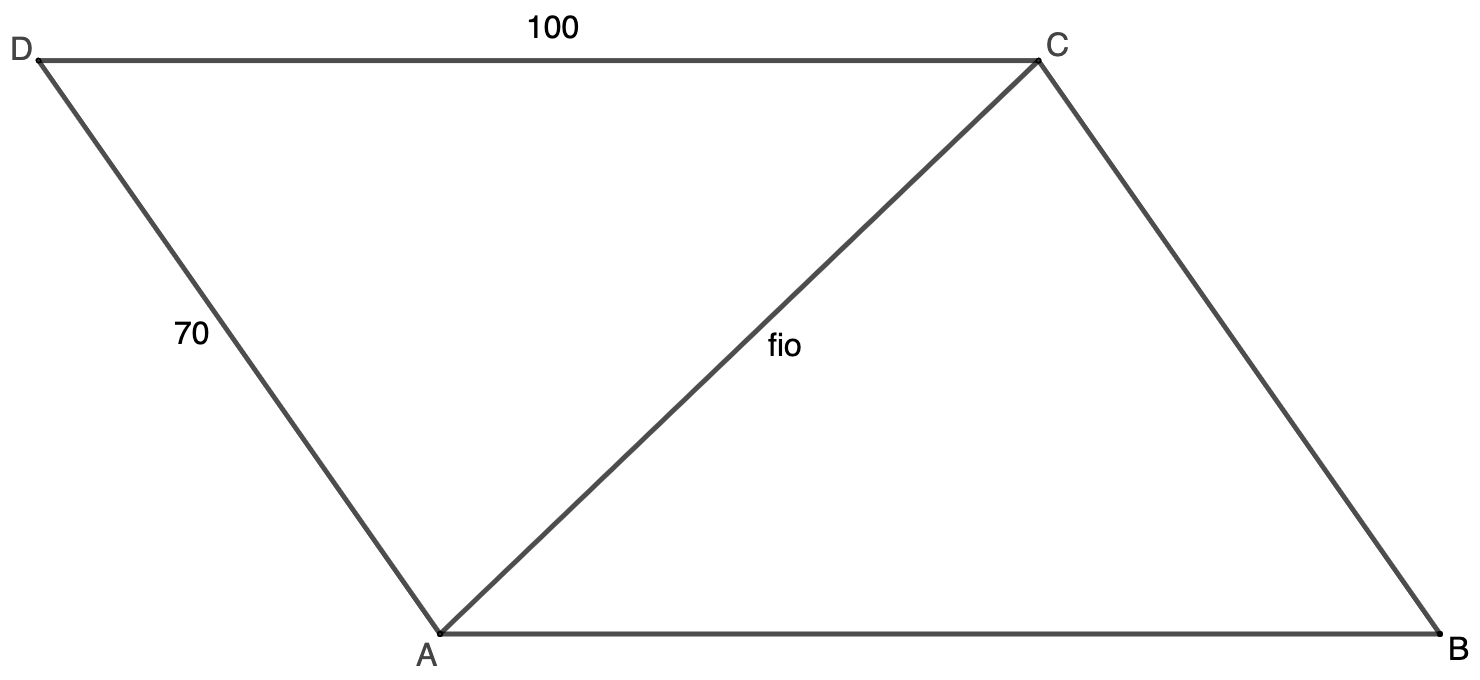
\includegraphics[scale=0.15]{sec2_atestacionamento2.png}
        \caption{Estacionamento em forma de paralelogramo $ABCD$.}
        \label{sec2_resatestacionamento2}
    \end{figure}

    \item{}
    Não podemos, pois o paralelogramo que modela a situação pode ter diversos ângulos internos. 

    \item{}
    A seguir faremos uma construção que mostra que neste caso é possível calcular o tamanho do fio.
    
    Vamos chamar de $B$ o vértice do paralelogramo que modela o estacionamento de forma que $A\hat{B}C=55^\circ$. Sendo assim, em relação ao triângulo $ABC$ são conhecidos dois de seus lados e o ângulo compartilhado por eles. Neste caso, usando a lei do cossenos, podemos calcular o lado oposto ao ângulo $55^\circ$, isto é, o comprimento do fio.
    Pela lei dos cossenos,
    $$AC^2=BA^2+BC^2-2\cdot BA\cdot BC\cdot \cos(55^\circ)=100^2+70^2-2\cdot100\cdot70\cdot \cos(55^\circ).$$
    Com o auxílio da tabela trigonométrica sabemos que $\cos(55^\circ)=0,57$. Logo,
    $$AC^2=100^2+70^2-2\cdot100\cdot70\cdot 0,57 \iff AC=2\sqrt{1730}\text{m}.$$
    \begin{figure}[H]
        \centering
        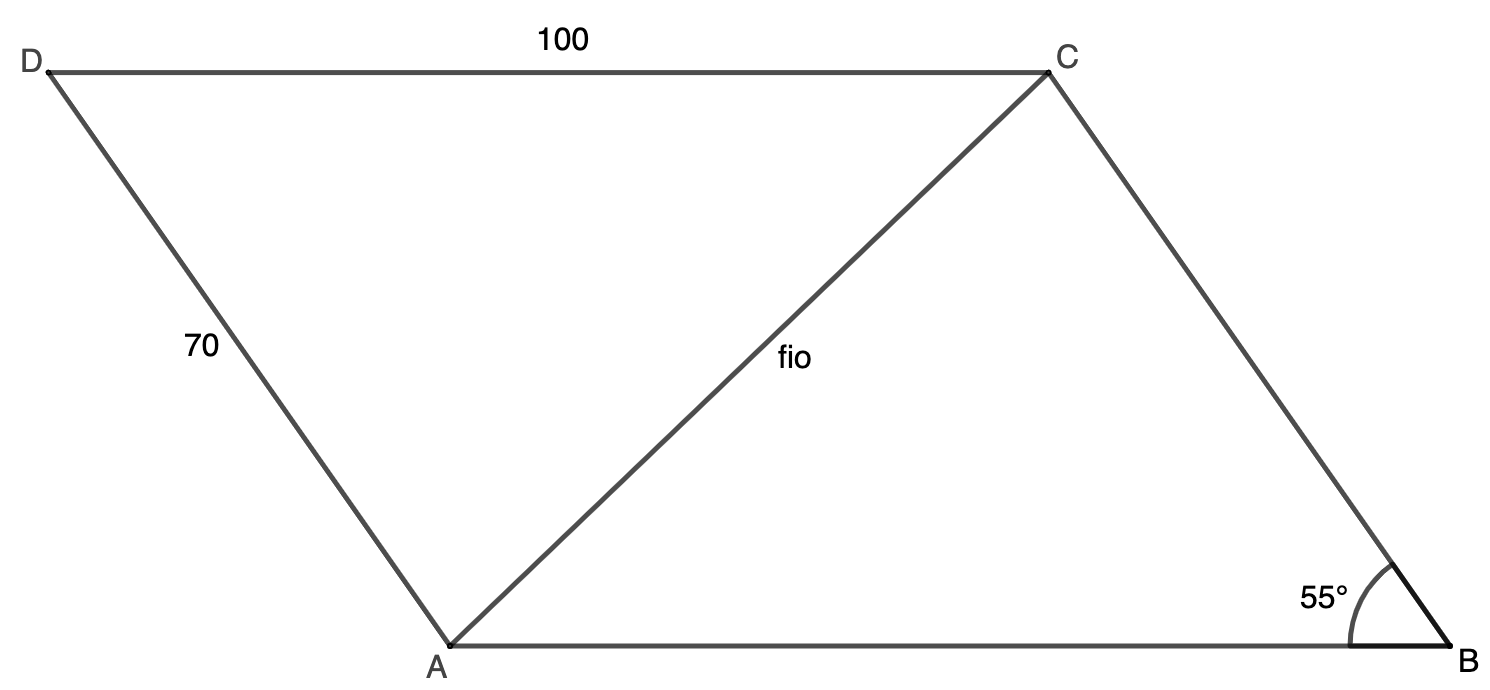
\includegraphics[scale=0.15]{sec2_atestacionamento3.png}
        \caption{Estacionamento em forma de um paralelogramo com um ângulo medindo $55^\circ$.}
        \label{sec2_resatestacionamento3}
    \end{figure}
    
    \item{}
    Sim, porque é possível determinar a medida do outro ângulo, já que em paralelogramos, ângulos adjacentes são complementares. Sendo assim, o ângulo $A\hat{B}C$ mede $125^\circ$. Neste caso, a lei dos cossenos nos daria o seguinte:
    $$AC^2=BA^2+BC^2-2\cdot BA\cdot BC\cdot \cos(125^\circ)=100^2+70^2-2\cdot100\cdot70\cdot \cos(125^\circ).$$
    Novamente utilizando a tabela trigonométrica, encontramos que $\cos(125^\circ)=-0,57$. Assim,
    $$AC^2=100^2+70^2-2\cdot100\cdot70\cdot (-0,57) \iff AC=4\sqrt{1430}\text{m}.$$
    \begin{figure}[H]
        \centering
        \includegraphics[scale=0.15]{sec2_atestacionamento4.png}
        \caption{Estacionamento em forma de um paralelogramo com um ângulo medindo $125^\circ$.}
        \label{sec2_resatestacionamento4}
    \end{figure}
\end{enumerate}
}{9}
\end{answer}

\clearmargin
\begin{objectives}{Molécula de água líquida e congelada}
{
\begin{itemize}
\item Utilizar a lei dos cossenos para resolver um problema contextualizado na área de Química e interpretar os resultados matemáticos obtidos diante da situação real estudada.

\item \textbf{Conceitos abordados}: lei dos cossenos, além de conceitos da Química, como átomos, moléculas e ângulo de ligação entre os átomos.
\end{itemize}
}{1}{2}
\end{objectives}
\begin{sugestions}{Molécula de água líquida e congelada}
{
Nesta atividade serão utilizados os seguintes dados, que poderão ser acessados pelos estudantes na tabela trigonométrica do fim do capítulo: $\arccos({0,25})=75^\circ$ e $\arccos({0,33})=71^\circ$. 

\textbf{Organização da turma}: em duplas.

\textbf{Dificuldades previstas}: destacamos mais uma vez ser necessário ter atenção ao uso adequado da lei dos cossenos em relação ao ângulo considerado. Além disso, nesta atividade, os estudantes podem ter dificuldades com os termos utilizados em Química, como átomos, moléculas, ligação entre átomos e etc. Sugerimos ao professor que esteja preparado para intervir caso seja constatada tal dificuldade e, sendo necessário, o professor de Química dos estudantes pode ser chamado para uma conversa conjunta. Neste caso, pode-se solicitar que o vocabulário usado na questão seja trabalhado, destacando o quanto as áreas de Matemática e Química estão relacionadas.
}{1}{2}
\end{sugestions}
\begin{answer}{Molécula de água líquida e congelada}
{
\begin{enumerate}
    \item{} A \Fref{sec2_resatquimica2} mostra um esquema  para a representação da molécula de água. 
    \begin{figure}[H]
        \centering
        \includegraphics[scale=0.3]{sec2_atquimica2.png}
        \caption{Esquema para representação de uma molécula de água.}
        \label{sec2_resatquimica2}
    \end{figure}
     
    \item{}
    Queremos encontrar o ângulo $H_1\hat{O}H_2$. Como conhecemos os três lados desse triângulo do $OH_1H_2$, usando a lei dos cossenos, podemos obter informações sobre um ângulo do triângulo. Usando, então, a lei dos cossenos de modo a obter o cosseno do ângulo $H_1\hat{O}H_2$, temos
    $$(H_1H_2)^2=(OH_1)^2+(OH_2)^2-2\cdot OH_1\cdot OH_2\cdot\cos({H_1\hat{O}H_2}).$$
    Substituindo os valores dos lados do triângulo $OH_1H_2$ na equação acima:
    $$151,8^2=96^2+96^2-2\cdot 96\cdot 96\cdot\cos({H_1\hat{O}H_2}) \iff \cos({H_1\hat{O}H_2})=-0,25.$$
    
    Como o ângulo ${H_1\hat{O}H_2}$ possui cosseno igual a $-0,25$, precisamos lembrar que se $\cos(H_1\hat{O}H_2)=\cos(180^\circ-\alpha)=-0,2501$, então 
    $$-\cos\alpha=\cos(180^\circ-\alpha)=-0,25 \iff \cos\alpha=0,25.$$
    Logo, $\alpha$ mede aproximadamente $75^\circ$, de acordo com a tabela trigonométrica do final do capítulo. Sendo assim, $H_1\hat{O}H_2$ mede aproximadamente $180^\circ-\alpha=180^\circ-75^\circ=105^\circ.$
    
    \item{}
    A \Fref{sec2_resatquimica2} mostra um esquema  para a representação da molécula de água usando os novos valores das distâncias entre os átomos.
    \begin{figure}[H]
        \centering
        \includegraphics[scale=0.3]{sec2_atquimica3.png}
        \caption{Esquema para representação de uma molécula de água.}
        \label{sec2_resatquimica3}
    \end{figure}
    Seguindo o mesmo caminho da questão anterior, temos que
    $$165^2=101^2+101^2-2\cdot 101\cdot 101\cdot\cos({H_1\hat{O}H_2}) \iff \cos({H_1\hat{O}H_2})=-0,33.$$
    
    Como o ângulo ${H_1\hat{O}H_2}$ possui cosseno igual a $-0,33$, análogo ao que foi feito no item anterior, precisamos lembrar que se $\cos(H_1\hat{O}H_2)=\cos(180^\circ-\alpha)=-0,33$, então 
    $$-\cos\alpha=\cos(180^\circ-\alpha)=-0,3344 \iff \cos\alpha=0,33.$$
    Logo, $\alpha$ mede aproximadamente $71^\circ$, de acordo com a tabela trigonométrica do final do capítulo. Sendo assim, $H_1\hat{O}H_2$ mede aproximadamente $180^\circ-\alpha=180^\circ-71^\circ=109^\circ.$
    
    \item{}
    Como visto nos dois itens anteriores, o ângulo da molécula de água aumenta quando ela é congelada. Mesmo sendo o triângulo um elemento geométrico plano, podemos conjecturar que esse aumento do ângulo se reflete no aumento do volume da água quando congelada. 
\end{enumerate}
}{9}
\end{answer}
\def\currentcolor{session4}

\begin{example}{Distância entre as margens de um lago} \label{sec2_leidoscossenos_ex}

(UERJ-2017) Ao coletar os dados para um estudo topográfico da margem de um lago a partir dos pontos $A, B$ e $T$, um técnico determinou as medidas $AT = 32$m, $BT = 13$m e $A\hat{T}B = 120^\circ$, representadas na \Fref{Lago}.
\begin{figure}[H]
    \centering
    \includegraphics[scale=0.65]{Lago.JPG}
    \caption{Lago.}
    \label{Lago}
\end{figure}
Calcule a distância, em metros, entre os pontos $A$ e $B$, definidos pelo técnico nas margens desse lago.

\paragraph{Solução}
\phantomsection\label{LA_sec2_leidoscossenos_exres}
Para encontrar a distância entre os pontos $A$ e $B$, podemos utilizar diretamente a lei dos cossenos no triângulo $ATB$, sendo $A\hat{T}B$ o ângulo a ser utilizado já que é o único conhecido no triângulo.

Para utilizar o ângulo $A\hat{T}B$, a lei dos cossenos se aplica ao triângulo $ATB$ da seguinte forma:
$$AB^2=AT^2+BT^2-2\cdot AT\cdot BT\cdot\cos(A\hat{T}B),$$ 
ou seja,
\begin{equation}
    AB^2=32^2+13^2-2\cdot32\cdot13\cdot\cos120^\circ. \label{sec2_leidoscossenos_ex_eq1}
\end{equation}

Pela definição de cossenos de ângulo obtuso,
$$\cos120^\circ=-\cos60^\circ=-\fra12.$$
Logo, substituindo esse valor da equação \eqref{sec2_leidoscossenos_ex_eq1}, concluímos que
$$AB^2=1024+169-832\cdot\left(-\fra12\right)=1609.$$
Sendo assim, $AB=\sqrt{1609}$m, ou seja, a distância entre os pontos $A$ e $B$ é de aproximadamente $40,11$m.
\end{example}

\practice{Praticando a lei dos cossenos}\label{prat_leidoscossenos}

\begin{task}{Estudando as câmeras de segurança de um estacionamento}
Atualmente, é muito comum encontrarmos câmeras de segurança em diversos locais que frequentamos diariamente. 
%
Além de aumentarem a segurança dos locais, as câmeras têm por finalidade auxiliar na identificação de objetos esquecidos, controle de grandes aglomerações de pessoas, etc. Em muitos desse locais, costuma-se utilizar as câmeras aos pares,  em posições opostas, garantindo, assim, o alcance de todo o espaço do estacionamento (\Fref{sec2_at_fig_camseguranca1}). 
 
\begin{figure}[H]
    \centering
    \includegraphics[scale=0.35]{sec2_at_enunciado_camseguranca1.png}
    \caption{Posicionamento de câmeras de segurança. Fonte: https://bit.ly/310nJFS.}
    \label{sec2_at_fig_camseguranca1}
\end{figure}

\begin{enumerate}
    \item{}
    Em um estacionamento com formato retangular de comprimento $100$m e largura $70$m serão instaladas duas câmeras de segurança em vértices opostos do estacionamento. Essas duas câmeras serão interligadas subterraneamente por um fio posicionado totalmente esticado, ou seja, em linha reta. Faça um esboço da situação, nomeando de $A$ e $C$ os vértices por onde passarão os fios que ligam essas câmeras.

    \item{}
    Apenas com os dados fornecidos no item anterior, é possível calcular o comprimento da parte subterrânea do fio que fará a ligação entre as câmeras? Se sim, encontre o seu comprimento.

    \item{}
    Imagine agora que, por razões técnicas, o estacionamento de um determinado shopping tenha o formato de um paralelogramo cujos lados medem $100$m e $70$m. Faça um esboço da situação, nomeando de $A$ e $C$ os vértices por onde passarão os fios que ligam essas câmeras.

    \item{}
    Apenas com os dados fornecidos no item anterior, é possível calcular o comprimento da parte subterrânea do fio que fará a ligação entre as câmeras? Se sim, encontre o comprimento.

    \item{}
    Considere agora que um dos ângulos do paralelogramo que determina o formato do estacionamento é $55^\circ$ e que o fio ficará oposto a esse ângulo. Nesse caso, é possível calcular o comprimento da parte subterrânea do fio que fará a ligação entre as câmeras? Se sim, encontre o comprimento.
    
    \item{}
    E se, ao contrário do considerado anteriormente, o fio cortasse o ângulo de $55^\circ$ que mencionamos no item anterior? Nesse caso, é possível calcular o comprimento da parte subterrânea do fio que fará a ligação entre as câmeras? Se sim, encontre o comprimento.
\end{enumerate}
\end{task}

\begin{task}{Molécula de água líquida e congelada}\label{sec2_leidoscossenos_atquimica}
Uma molécula de água é formada por dois átomos de hidrogênio e um átomo de oxigênio. A ligação entre os átomos de hidrogênio e de oxigênio faz com que a molécula da água tenha sempre formato triangular, independente de seu estado. Quando em estado líquido, a distância entre o átomo de oxigênio e o átomo de hidrogênio é de 96 picômetros e entre os dois átomos de hidrogênio é 151,8 picômetros ($1$ picômetro corresponde à $10^{-12}$ metros). Utilizando esses dados, faça o que se pede.

Caso seja necessário, utilize 2 casas decimais para calcular as aproximações pedidas.

\begin{enumerate}
    \item{}
    Faça um esquema que represente uma molécula de água, considerando que não há ligação entre os átomos de hidrogênio. O átomo de oxigênio deve ser denotado por $O$, enquanto os dois átomos de hidrogênio devem ser denotados por $H_1$ e $H_2$.
    
    \item{}
    Encontre o ângulo de ligação entre os átomos da molécula de água, ou seja, o ângulo $H_1\hat{O}H_2$.
    
    \item{}
    Quando a água congela, a distância entre o átomo de oxigênio e o átomo de hidrogênio é alterada para 101 picômetros e entre os dois átomos de hidrogênio para 165 picômetros. Encontre o ângulo de ligação entre os átomos da molécula de água nesta nova situação.

    \item{}
    Podemos perceber que, quando a água congela, ela tende a aumentar seu volume. Tente relacionar essa informação com o que foi calculado anteriormente.  
\end{enumerate}
\end{task}

\know{}
A lei dos cossenos nos trouxe uma equação que relaciona lados e o ângulos de um triângulo qualquer. A partir desse resultado, conseguimos relacionar também o tipo de triângulo com os tamanhos de seus lados da seguinte forma: 

Se $ABC$ um triângulo onde $AB=c, BC=a$ e $AC=b$. Se $a>b>c$, então
\begin{enumerate}
    \item{}
    $ABC$ é retângulo $\iff a^2=b^2+c^2$.
    
    \item{}
    $ABC$ é acutângulo $\iff a^2<b^2+c^2$.
    
    \item{}
    $ABC$ é obtusângulo $\iff a^2>b^2+c^2$.
\end{enumerate}

Por que isso é verdade?

\begin{enumerate}
    \item{}
    Utilizando a lei dos cossenos, temos que 
    $$\begin{array}{ccl}
        a^2 = b^2+c^2 & \iff & b^2+c^2-2bc\cos (C\hat{A}B) = b^2+c^2 \\
                      & \iff & -2bc\cos (C\hat{A}B)= 0\\
                      & \iff & \cos (C\hat{A}B)=0\\
                      & \iff & C\hat{A}B=90^\circ.
    \end{array}$$
    Este primeiro item, na verdade, é o teorema de Pitágoras e sua recíproca. 
    
    Vale a pena frisar que, a recíproca do teorema de Pitágoras diz que, se a igualdade $a^2=b^2+c^2$ é satisfeita para um triângulo $ABC$ onde $AB=c, BC=a$ e $AC=b$, então esse triângulo é retângulo em $A$.
    
    \item{}
    Utilizando a lei dos cossenos, temos que 
    $$\begin{array}{ccl}
        a^2 < b^2+c^2 & \iff & b^2+c^2-2bc\cos (C\hat{A}B)< b^2+c^2 \\
                      & \iff & -2bc\cos (C\hat{A}B)< 0\\
                      & \iff & \cos (C\hat{A}B)>0\\
                      & \iff & C\hat{A}B<90^\circ.
    \end{array}$$
    
    \item{}
    Analogamente ao que foi feito anteriormente, vamos utilizar a lei dos cossenos: 
    $$\begin{array}{ccl}
        a^2 > b^2+c^2 & \iff & b^2+c^2-2bc\cos (C\hat{A}B) > b^2+c^2 \\
                      & \iff & -2bc\cos (C\hat{A}B) > 0\\
                      & \iff & \cos (C\hat{A}B) < 0\\
                      & \iff & C\hat{A}B > 90^\circ.
    \end{array}$$
\end{enumerate}

\cleardoublepage
\def\currentcolor{session1}
\begin{objectives}{Medindo distâncias inacessíveis}
{
\begin{itemize}
\item Aplicar a argumentação utilizada na lei dos senos, que será apresentada adiante, na solução de um problema numérico e adquirir familiaridade com este tipo de argumentação antes de sua formalização.

\item \textbf{Conceitos abordados}: razões trigonométricas e lei dos cossenos.
\end{itemize}
}{1}{1}
\end{objectives}
\begin{sugestions}{Medindo distâncias inacessíveis}
{
Esta atividade tem por finalidade apresentar os passos da demonstração da lei dos senos em um contexto numérico. 
%
Com o desenvolvimento dessa atividade, acreditamos que os estudantes compreenderão de forma mais natural esta demonstração. 
%
Além disso, sugerimos ao professor que estimule o aluno a construir uma estratégia de resolução a partir de seus dados, antes de realizar os cálculos de uma questão. Por exemplo, o estudante deve perceber que não há possibilidade de utilizar a lei dos cossenos pelos dados fornecidos no enunciado.

Nesta atividade serão utilizados os seguintes dados, que poderão ser acessados pelos estudantes na tabela trigonométrica do fim do capítulo: $\sen(62^\circ)=0,88, \sen(48^\circ)=0,74$ e $\sen(70^\circ)=0,93$.

\textbf{Organização da turma}: em duplas.
}{1}{1}
\end{sugestions}
\begin{answer}{Medindo distâncias inacessíveis}
{
Notemos, primeiramente, que precisamos calcular a altura do drone em cada uma das posições apresentadas nos itens da atividade para determinar se ele produzirá imagens com boa qualidade onde está posicionado. Para isso, vamos trabalhar com um triângulo onde dois de seus vértices coincidem com os córneres diametralmente opostos do campo, digamos $A$ e $B$, e o terceiro vértice do triângulo com a posição do drone, digamos $C$. Sendo assim, queremos encontrar a altura do triângulo $ABC$ a partir do vértice $C$. 

Em cada uma das situações apresentadas,  conhecemos dois ângulos internos do triângulo $ABC$ e, consequentemente o terceiro também. Além disso, podemos calcular a medida do segmento $AB$, que coincide com a diagonal do campo em forma retangular, através do teorema de Pitágoras:
$$AB^2=90^2+120^2=22500 \iff AB=150\text{m}.$$ 
Neste caso, estamos trabalhando com um triângulo como o da \Fref{sec2_at_drone_resolucao1_fig}, onde os ângulos internos dependem de cada situação. 
\begin{figure}[H]
    \centering
    \includegraphics[scale=0.6]{sec2_at_drone_resolucao1.png}
    \caption{Triângulo $ABC$.}
    \label{sec2_at_drone_resolucao1_fig}
\end{figure}

\begin{enumerate}
\item{}
Neste primeiro item, o drone está posicionado acima do centro do campo, de modo que seja visto de córneres diametralmente opostos por um ângulo de $45^\circ$. Neste caso, modelando a situação pelo triângulo $ABC$, como já discutido anteriormente, temos que os ângulos $C\hat{A}B$ e $A\hat{B}C$ devem medir $45^\circ$.

Neste caso, como a soma dos ângulos internos de um triângulo qualquer é $180^\circ$, o ângulo $A\hat{C}B$ mede $90^\circ$. Assim, o triângulo $ABC$ é isósceles de base $AB$ e retângulo em $C$, como vemos na \Fref{sec2_at_drone_resolucao_itema_1_fig}.
\begin{figure}[H]
    \centering
    \includegraphics[scale=0.6]{sec2_at_drone_resolucao_itema_1.png}
    \caption{Triângulo $ABC$.}
    \label{sec2_at_drone_resolucao_itema_1_fig}
\end{figure}

Seja $CD$ a altura de $ABC$ a partir do vértice $C$ e $h$ sua medida. Como $ABC$ é isósceles, sabemos que sua altura divide a base em dois segmentos de mesmo comprimento. Logo, as medidas de $AD$ e $DB$ são iguais a $75$m. Veja a \Fref{sec2_at_drone_resolucao_itema_2_fig}.
\begin{figure}[H]
    \centering
    \includegraphics[scale=0.6]{sec2_at_drone_resolucao_itema_2.png}
    \caption{Triângulo $ABC$.}
    \label{sec2_at_drone_resolucao_itema_2_fig}
\end{figure}

Note que o triângulo $ADC$ é retângulo em $D$ e seu ângulo interno $C\hat{A}D$ mede $45^\circ$. Logo, como a soma dos ângulos internos de um triângulo qualquer é $180^\circ$, a medida de $A\hat{C}D$ é também $45^\circ$. Ou seja, $ADC$ é isósceles de base $AC$. Sendo assim, a medida dos lados $AD$ e $CD$ são iguais. Portanto, $h=75$m.

Assim, o drone está a uma altura de $75$m e abaixo do limite estipulado para gerar boas imagens.

\item{}
Nesta nova situação, análogo ao que tínhamos no item anterior, vemos que $ABC$ possui ângulos internos $C\hat{A}B, A\hat{B}C$ e $B\hat{C}A$ medindo $70^\circ, 62^\circ$ e $48^\circ$, respectivamente. Além disso, conhecemos a medida de $AB$, que é $150$m. Veja a \Fref{sec2_at_drone_resolucao_itemb_1_fig}.
\begin{figure}[H]
    \centering
    \includegraphics[scale=0.6]{sec2_at_drone_resolucao_itemb_1.png}
    \caption{Triângulo $ABC$.}
    \label{sec2_at_drone_resolucao_itemb_1_fig}
\end{figure}

Sejam $CD$ a altura do triângulo $ABC$ traçada a partir de $C$ e $h$ sua medida. Tracemos a altura $AE$ do triângulo $ABC$ a partir do vértice $A$ e denotemos sua medida por $h'$. A situação está esboçada na \Fref{sec2_at_drone_resolucao_itemb_2_fig}.
\begin{figure}[H]
    \centering
    \includegraphics[scale=0.6]{sec2_at_drone_resolucao_itemb_3.png}
    \caption{Triângulo $ABC$ com alturas $CD$ e $AE$.}
    \label{sec2_at_drone_resolucao_itemb_2_fig}
\end{figure}

No triângulo retângulo $ABE$, temos que:
\begin{equation}
    \sen(62^\circ)=\fra{AE}{AB}=\fra{h'}{150},\label{sec2_at_drone_itema_eq1}
\end{equation}
e no triângulo retângulo $CAE$, temos que:
\begin{equation}
    \sen(48^\circ)=\fra{AE}{AC}=\fra{h'}{AC}.\label{sec2_at_drone_itema_eq2}
\end{equation}

De \eqref{sec2_at_drone_itema_eq1} e \eqref{sec2_at_drone_itema_eq2}, temos que
$$150\cdot\sen(62^\circ)=AC\cdot\sen(48^\circ).$$
Logo, 
\begin{equation}
    \fra{\sen(48^\circ)}{150}=\fra{\sen(62^\circ)}{AC}.\label{sec2_at_drone_itema_eq3}
\end{equation}
Substituindo os valores de $\sen(62^\circ)=0,88$ e $\sen(48^\circ)=0,74$ encontrados na tabela trigonométrica do final do capítulo e aproximados por duas casas decimais, na equação acima encontramos:
$$\fra{0,74}{150}=\fra{0,88}{AC} \iff AC=178,37\text{m}.$$

No triângulo $CAD$, temos
$$\sen(70^\circ)=\fra{CD}{AC}.$$
Usando novamente a tabela trigonométrica encontramos $\sen(70^\circ)=0,93$, que pode ser substituído na equação acima para encontrar o seguinte:
$$0,93=\fra{CD}{178,37} \iff CD=165,88\text{m}.$$
Sendo assim, a altura do drone é $165,88$m e podemos concluir que as imagens feitas por ele não terão qualidade suficiente para a exibição das imagens no canal de televisão.
\end{enumerate}
}{9}
\end{answer}

\explore{Trabalhando com um triângulo qualquer}\label{exp_outrarelacaonotriangulo}
Vimos anteriormente que a lei dos cossenos estende o teorema de Pitágoras, na medida em que fornece uma relação válida em um triângulo qualquer e que recai sobre o teorema de Pitágoras quando se trata de um triângulo retângulo. Nesta seção, mostraremos que podemos construir uma outra relação válida em um triângulo qualquer, mas que difere da lei dos cossenos por utilizar diferentes informações do triângulo.

\begin{task}{Medindo distâncias inacessíveis}
Um drone está sobrevoando um campo de futebol em formato retangular para fazer imagens de um jogo que será transmitido por um canal de televisão. Segundo especialistas em geração de imagem, a altura máxima deste drone para que as imagens possam ter boa qualidade é de $150$m. Considere que o campo possui $120$m de comprimento e $90$m de largura para responder as perguntas a seguir.

Se for preciso, faça aproximações de valores decimais com duas casas decimais.

\begin{enumerate}
    \item{}
    Caso o drone esteja posicionado acima do centro do campo, de modo que duas pessoas posicionadas em dois córneres do campo diametralmente opostos o vejam por um ângulo de $45^\circ$, as imagens produzidas pelo drone desta posição terão boa qualidade?
    
    Dizer que o drone é visto por um ângulo de $45^\circ$ significa que o ângulo entre o segmento que liga os dois córneres onde estão posicionadas as pessoas e o segmento que liga os pés da pessoa posicionada sobre um córner e o drone é $45^\circ$. Veja a \Fref{sec2_leidossenos_atdrone_fig1}.
    \begin{figure}[H]
    \centering
    \includegraphics[scale=0.6]{sec2_at_drone_enunciado.png}
    \caption{Drone posicionado sobre um campo de futebol (Esta figura é apenas ilustrativa da situação, mas precisaremos de uma figura feita pelo designer contendo o campo, o drone e etc.). 
    }
    \label{sec2_leidossenos_atdrone_fig1}
\end{figure}

    
    \item{}
    Agora, considere que o drone esteja posicionado em um ponto qualquer acima do campo, de forma que duas pessoas posicionadas em dois córneres do campo diametralmente opostos o vejam por ângulos de $70^\circ$ e $62^\circ$. Neste caso, as imagens produzidas desta posição terão boa qualidade? 
\end{enumerate}
\end{task}

\arrange{Lei dos Senos}

Aplicando a lei dos cossenos a um triângulo qualquer, podemos determinar a medida de seus lados, caso sejam conhecidos os outros dois e o ângulo entre eles, ou de seus ângulos, caso sejam conhecidas as medidas de seus três lados. Mas, se conhecemos apenas a medida de um lado e de dois ângulos de um triângulo, não é possível aplicar a lei dos cossenos. Nesta seção, o objetivo é encontrar uma nova relação válida para qualquer triângulo envolvendo as medidas dos lados e dos ângulos de um triângulo qualquer.  Esta relação será chamada lei dos senos.

Primeiramente, enunciaremos e demonstraremos a lei dos senos para triângulos acutângulos. Mais adiante, estenderemos esse resultado para triângulos retângulos e obtusângulos.

\begin{observationtitle}{Lei dos Senos - Parte 1}
\phantomsection\label{sec2_leidossenos}
Seja $ABC$ um triângulo acutângulo, onde $a, b$ e $c$ são as medidas dos lados $BC, AC$ e $AB$, e $\alpha, \beta, \gamma$ são as medidas dos ângulos $B\hat{A}C,C\hat{B}A$ e $A\hat{C}B$, respectivamente (\Fref{sec2_leidossenos_parte1_demo_enunciado_fig}). Então,
\begin{equation}\label{sec2_leidossenos_eq_parte1}
    \frac{a}{\sen\alpha} = \frac{b}{\sen\beta} = \frac{c}{\sen\gamma}.
\end{equation}
\begin{figure}[H]
    \centering
    \includegraphics[scale=0.7]{sec2_leidossenos_parte1_enunciado.png}
    \caption{$ABC$ é um triângulo acutângulo como do enunciado da lei dos senos - parte 1.}
    \label{sec2_leidossenos_parte1_demo_enunciado_fig}
\end{figure}
\end{observationtitle}

\paragraph{Demonstração da Lei dos Senos - Parte 1}

Considere, então, o triângulo acutângulo $ABC$, como mostrado na \Fref{sec2_leidossenos_parte1_demo_enunciado_fig}.

Seja $CD$ a altura do triângulo $ABC$ traçada a partir do vértice $C$ e $h$ sua medida. Veja a \Fref{sec2_leidossenos_parte1_demo1_fig}.
\begin{figure}[H]
    \centering
    \includegraphics[scale=0.7]{sec2_leidossenos_parte1_demo1.png}
    \caption{$ABC$ é um triângulo acutângulo com altura $CD$.}
    \label{sec2_leidossenos_parte1_demo1_fig}
\end{figure}

No triângulo $CBD$, temos que 
\begin{equation}
\sen\beta=\fra{CD}{BC}=\fra{h}{a}.    \label{sec2_leidossenos_demo_parte1_eq1}
\end{equation}
E, no triângulo $CAD$, temos que
\begin{equation}
\sen\alpha=\fra{CD}{AC}=\fra{h}{b}.    \label{sec2_leidossenos_demo_parte1_eq2}
\end{equation}

De \eqref{sec2_leidossenos_demo_parte1_eq1} e \eqref{sec2_leidossenos_demo_parte1_eq2}, vemos que
$$a \sen\beta = b \sen\alpha.$$
Logo,
\begin{equation}
\fra{\sen\alpha}{a}=\fra{\sen\beta}{b}.    \label{sec2_leidossenos_demo_parte1_eq3}
\end{equation}

Agora, seja $AE$ a altura do triângulo $ABC$ traçada a partir de $A$ e denotemos por $h'$ sua medida. A situação está esboçada na \Fref{sec2_leidossenos_parte1_demo2_fig}.
\begin{figure}[H]
    \centering
    \includegraphics[scale=0.75]{sec2_leidossenos_parte1_demo2.png}
    \caption{$ABC$ é um triângulo acutângulo com altura $AE$.}
    \label{sec2_leidossenos_parte1_demo2_fig}
\end{figure}

No triângulo $ACE$, temos que 
\begin{equation}
\sen\gamma=\fra{AE}{AC}=\fra{h'}{b}.    \label{sec2_leidossenos_demo_parte1_eq4}
\end{equation}
E, no triângulo $ABE$, temos que
\begin{equation}
\sen\beta=\fra{AE}{AB}=\fra{h'}{c}.    \label{sec2_leidossenos_demo_parte1_eq5}
\end{equation}

De \eqref{sec2_leidossenos_demo_parte1_eq4} e \eqref{sec2_leidossenos_demo_parte1_eq5}, vemos que
$$b \sen\gamma = c \sen\beta.$$
Logo,
\begin{equation}
\fra{\sen\beta}{b}=\fra{\sen\gamma}{c}.    \label{sec2_leidossenos_demo_parte1_eq6}
\end{equation}

Unindo \eqref{sec2_leidossenos_demo_parte1_eq3} e \eqref{sec2_leidossenos_demo_parte1_eq6}, obtemos
$$\frac{a}{\sen\alpha} = \frac{b}{\sen\beta} = \frac{c}{\sen\gamma},$$
como desejado.


Agora, nosso desafio é compreender se é possível encontrar um resultado semelhante ao encontrado na lei dos senos - parte 1 para triângulos retângulos e obtusângulos. É importante ressaltar que, a relação encontrada anteriormente envolve o seno dos ângulos internos do triângulo. Isso não foi um problema, já que trabalhamos com um triângulo acutângulo e portanto, seus ângulos internos são todos agudos. E, para ângulos agudos, já sabemos como calcular seu seno. 

Agora, queremos generalizar este resultado para qualquer triângulo. Para isso, precisamos trabalhar com triângulos retângulos e obtusângulos e neste caso, será necessário calcular o seno de ângulos retos e obtusos, além de agudos. Para, então, proceder com essa extensão da lei dos senos, vamos ampliar a definição de seno de um ângulo agudo para um ângulos qualquer entre $0^\circ$ e $180^\circ$, como fizemos com o cosseno desses mesmos ângulos ao trabalhar a lei dos cossenos. 

Definimos:
\begin{itemize}[topsep=0pt, itemsep=0pt]
\item $\sen(0^\circ)= 0$;
\item $\sen(90^\circ)= 1$;
\item $\sen(180^\circ)= 0$;
\item para um ângulo obtuso $\alpha$, $\sen\alpha=\sen(180^\circ-\alpha).$
\end{itemize}

Nesta definição, utilizamos o seno de $180^\circ-\alpha$ para definir o seno de $\alpha$. Observe que se $\alpha$ é um ângulo obtuso, então $180^\circ-\alpha$ é um ângulo agudo e portanto, sabemos calcular seu seno com o conteúdo que aprendemos até aqui. 

\begin{observation}
Já sabemos que o seno de um ângulo agudo $\alpha$ assume apenas valores positivos e menores que $1$, então, de acordo com a definição acima,  
$$\text{se }0^\circ \leq\alpha \leq180^\circ, \text{então} 0\leq\sen\alpha\leq 1.$$
\end{observation}

No que se segue, utilizaremos a definição anterior para trabalhar com o seno de ângulos entre $0^\circ$ e $180^\circ$. Como já mencionado anteriormente, caso você queira saber um pouco mais sobre essa definição, veja o \textit{Para saber+ Explorando a definição de senos e cossenos}. 

\begin{observationtitle}{Relação Fundamental para ângulos entre $0^\circ$ e $180^\circ$}
Antes de prosseguir com o estudo da generalização da lei dos senos, já que agora sabemos calcular o seno e cosseno de $0^\circ, 90^\circ, 180^\circ$ e de ângulos obtusos, vamos discutir se a relação fundamental válida para ângulos agudos pode ser estendida para qualquer ângulo entre $0^\circ$ e $180^\circ$:

$\bullet$ se $\sen(0^\circ)= 0$ e $\cos(0^\circ)= 1$, então $\sen^2(0^\circ)+\cos^2(0^\circ)=1$;

$\bullet$ se $\sen(90^\circ)= 1$ e $\cos(90^\circ)= 0$, então $\sen^2(90^\circ)+\cos^2(90^\circ)=1$;

$\bullet$ se $\sen(180^\circ)= 0$ e $\cos(180^\circ)= -1$, então $\sen^2(180^\circ)+\cos^2(180^\circ)=1$;

$\bullet$ se $\alpha$ é um ângulo obtuso onde  $\sen\alpha=\sen(180^\circ-\alpha)$ e $\cos\alpha=-\cos(180^\circ-\alpha)$, então
\begin{equation}
  \sen^2\alpha+\cos^2\alpha=(\sen(180^\circ-\alpha))^2+(-\cos(180^\circ-\alpha))^2. \label{sec2_relacaofundamental_angobt1}  
\end{equation}

Como $\alpha$ é um ângulo obtuso, então $180^\circ-\alpha$ é um ângulo agudo e portanto, já conhecemos a relação fundamental que estabelece neste caso que
\begin{equation}
  \sen^2(180^\circ-\alpha)+\cos^2(180^\circ-\alpha)=1. \label{sec2_relacaofundamental_angobt2}  
\end{equation}

Por \eqref{sec2_relacaofundamental_angobt1} e \eqref{sec2_relacaofundamental_angobt2}, 
$$\sen^2\alpha+\cos^2\alpha=1.$$

Sendo assim, concluímos que, para todo ângulo $\alpha$ entre $0^\circ$ e $180^\circ$, vale que
$$\sen^2\alpha+\cos^2\alpha=1.$$
\end{observationtitle}

Como já sabemos calcular o seno de qualquer ângulo entre $0^\circ$ e $180^\circ$, então estamos prontos para  enunciar e demonstrar a lei dos senos para triângulos retângulos e obtusângulos. 

\begin{observationtitle}{Lei dos Senos - Parte 2}
\phantomsection\label{sec2_leidossenos_parte2}
Seja $ABC$ um triângulo retângulo em $A$ ou obtusângulo, onde $a, b$ e $c$ são as medidas dos lados $BC, AC$ e $AB$, e $\alpha, \beta, \gamma$ são as medidas dos ângulos $B\hat{A}C,C\hat{B}A$ e $A\hat{C}B$, respectivamente (\Fref{sec2_leidossenos_parte2_enunciado_fig}). Então,
\begin{equation}\label{sec2_leidossenos_eq_parte2}
    \frac{a}{\sen\alpha} = \frac{b}{\sen\beta} = \frac{c}{\sen\gamma}.
\end{equation}
\begin{figure}[H]
    \centering
    \includegraphics[scale=0.6]{sec2_leidossenos_parte2_demo3.png}
    \qquad
    \includegraphics[scale=0.6]{sec2_leidossenos_parte2_enunciado1.png}
    \caption{Triângulos $ABC$ retângulo (da esquerda) e obtusângulo (da direita) como do enunciado da lei dos senos - parte 2.}
    \label{sec2_leidossenos_parte2_enunciado_fig}
\end{figure}

\end{observationtitle}


\paragraph{Demonstração da Lei dos Senos - Parte 2}

Nesta demonstração, precisamos considerar que o triângulo $ABC$ pode ser retângulo ou obtusângulo, como mostra a \Fref{sec2_leidossenos_parte2_enunciado_fig}. Sendo assim, organizaremos esta demonstração em duas partes. 

Primeira parte: $ABC$ é retângulo em $A$.

Neste caso, estamos considerando que $\alpha=90^\circ$ (veja a \Fref{sec2_leidossenos_parte2_enunciado_fig}).

Observando o triângulo $ABC$, obtemos que:
\begin{eqnarray}
\sen\beta=\fra{AC}{BC}=\fra{b}{a} \iff a=\fra{b}{\sen\beta},   \label{sec2_leidossenos_demo_parte2_eq7} \\ 
\sen\gamma=\fra{AB}{BC}=\fra{c}{a} \iff a=\fra{c}{\sen\gamma}.   \label{sec2_leidossenos_demo_parte2_eq8} 
\end{eqnarray}

De \eqref{sec2_leidossenos_demo_parte2_eq7} e \eqref{sec2_leidossenos_demo_parte2_eq8}, encontramos
$$a=\fra{b}{\sen\beta}=\fra{c}{\sen\beta}.$$
Como, por definição, $\sen\alpha=\sen90^\circ=1$, então a equação acima pode ser reescrita da seguinda maneira: 
$$\fra{a}{\sen\alpha}=\fra{b}{\sen\beta}=\fra{c}{\sen\gamma},$$
que é a equação procurada.

Segunda parte: $ABC$ é obtusângulo.

Consideremos, então, o triângulo obtusângulo $ABC$, como mostrado na \Fref{sec2_leidossenos_parte2_enunciado_fig}.

Seja $CD$ a altura do triângulo $ABC$ traçada a partir do vértice $C$ e $h$ sua medida. Veja a \Fref{sec2_leidossenos_parte2_demo1_fig}.
\begin{figure}[H]
    \centering
    \includegraphics[scale=0.55]{sec2_leidossenos_parte2_demo1.png}
    \caption{$ABC$ é um triângulo obtusângulo com altura $CD$.}
    \label{sec2_leidossenos_parte2_demo1_fig}
\end{figure}

No triângulo $CDB$, temos que 
\begin{equation}
\sen\beta=\fra{CD}{BC}=\fra{h}{a}.    \label{sec2_leidossenos_demo_parte2_eq1}
\end{equation}
E, no triângulo $CAD$, temos que
\begin{equation}
\sen(180^\circ-\alpha)=\fra{CD}{AC}=\fra{h}{b}.    \label{sec2_leidossenos_demo_parte2_eq2}
\end{equation}

De \eqref{sec2_leidossenos_demo_parte2_eq1} e \eqref{sec2_leidossenos_demo_parte2_eq2}, vemos que
$$a \sen\beta = b \sen(180^\circ-\alpha).$$
Como $\sen(180^\circ-\alpha)=\sen\alpha$, temos
\begin{equation}
\fra{\sen\alpha}{a}=\fra{\sen\beta}{b}.    \label{sec2_leidossenos_demo_parte2_eq3}
\end{equation}

Agora, seja $AE$ a altura do triângulo $ABC$ traçada a partir de $A$ e denotemos por $h'$ sua medida. A situação está esboçada na \Fref{sec2_leidossenos_parte2_demo2_fig}.
\begin{figure}[H]
    \centering
    \includegraphics[scale=0.55]{sec2_leidossenos_parte2_demo2.png}
    \caption{$ABC$ é um triângulo obtusângulo com altura $AE$.}
    \label{sec2_leidossenos_parte2_demo2_fig}
\end{figure}

No triângulo $ACE$, temos que 
\begin{equation}
\sen\gamma=\fra{AE}{AC}=\fra{h'}{b}.    \label{sec2_leidossenos_demo_parte2_eq4}
\end{equation}
E, no triângulo $ABE$, temos que
\begin{equation}
\sen\beta=\fra{AE}{AB}=\fra{h'}{c}.    \label{sec2_leidossenos_demo_parte2_eq5}
\end{equation}

De \eqref{sec2_leidossenos_demo_parte2_eq4} e \eqref{sec2_leidossenos_demo_parte2_eq5}, vemos que
$$b \sen\gamma = c \sen\beta.$$
Logo,
\begin{equation}
\fra{\sen\beta}{b}=\fra{\sen\gamma}{c}.    \label{sec2_leidossenos_demo_parte2_eq6}
\end{equation}

Unindo \eqref{sec2_leidossenos_demo_parte2_eq3} e \eqref{sec2_leidossenos_demo_parte2_eq6}, obtemos
$$\frac{a}{\sen\alpha} = \frac{b}{\sen\beta} = \frac{c}{\sen\gamma},$$
como desejado.

Após estudar a parte 1 e a parte 2 da lei dos senos, concluímos que, dado um triângulo qualquer $ABC$, onde $a, b$ e $c$ são as medidas dos lados $BC, AC$ e $AB$, e $\alpha, \beta, \gamma$ são as medidas dos ângulos $B\hat{A}C,C\hat{B}A$ e $A\hat{C}B$, respectivamente, então
    $$\frac{a}{\sen\alpha} = \frac{b}{\sen\beta} = \frac{c}{\sen\gamma}.$$

Com esse resultado, encontramos então uma nova relação válida para um triângulo qualquer envolvendo as medidas dos ângulos e dos lados desse triângulo. Sendo assim, conhecemos dois resultados válidos em triângulos quaisquer que fornecem esse tipo de relação: lei dos cossenos e lei dos senos. A aplicabilidade de cada uma das leis será determinada pelos dados do problema a ser resolvido.

%%%%% Exemplo da lei dos senos
\begin{example}{Distância entre dois corredores} \label{sec2_leidossenos_exemplo}

Um corredor corre em linha reta partindo do ponto $A$ no sentido $AX$ e com velocidade constante igual à $v_S= 8,0$ m/s. Já um outro corredor, se desloca a partir de $B$ em linha reta no sentindo $BX$ e com velocidade constante igual à $v_B=8\sqrt{3}$ m/s, e pretende alcançar o corredor $A$ no ponto $X$. Veja a \Fref{sec2_leidossenos_ex_enunciado}.
\begin{figure}[H]
    \centering
    \includegraphics[scale=0.65]{sec2_leidossenos_ex_enunciado.png}
    \caption{Corredores partindo dos pontos $A$ e $B$.}
    \label{sec2_leidossenos_ex_enunciado}
\end{figure}

Supondo que os corredores partem simultaneamente de suas posições iniciais $A$ e $B$ e que o ângulo $B\hat{A}X$ mede $120^\circ$, determine a medida do ângulo $\alpha$ que a trajetória de $B$ deve fazer com o segmento $AB$ para que o encontro entre os dois corredores aconteça no ponto $X$.

\paragraph{Solução}
\phantomsection\label{sec2_leidossenos_exemplo_res}
 Antes de iniciarmos a questão, precisamos lembrar da Física que a distância percorrida por um corredor com velocidade constante $v$ em um intervalo de tempo $t$ é $d=v\cdot t$. Utilizaremos este fato mais adiante na resolução da atividade.
 
 Para que os corredores se encontrem no ponto $X$ tendo partido simultaneamente de suas posições iniciais $A$ e $B$, eles devem levar o mesmo intervalo de tempo $t$ para percorrer seus percursos. Assim, como $v_A= 8,0$ m/s e $v_B=8\sqrt{3}$ m/s são as velocidades dos corredores que partem de $A$ e $B$, respectivamente, a distância percorrida em metros por eles no intervalo de tempo $t$ é $8t$ (partindo de $A$) e $8\sqrt{3}t$ (partindo de $B$). 
 
 Neste caso, o triângulo $ABX$ possui o lado $AX$ medindo $8t$ e o lado $BX$ medindo $8\sqrt{3}t$. Veja a \Fref{sec2_leidossenos_ex_resolucao}.
  \begin{figure}[H]
    \centering
    \includegraphics[scale=0.7]{sec2_leidossenos_ex_res1.png}
    \caption{Trajetórias dos corredores $C_1$ e $C_2$.}
    \label{sec2_leidossenos_ex_resolucao}
\end{figure}

Neste caso, estamos interessadas em encontrar o ângulo $\alpha$, mas não conhecemos todos os lados do triângulo. Por isso, não podemos utilizar a lei dos cossenos. Porém, como conhecemos a medida dos lados opostos aos ângulos $\alpha$ e $B\hat{A}X$, então a lei dos senos é a indicada para resolver o problema.
    
    Usando a lei dos senos no triângulo $ABX$, segue que:
    $$\frac{8t}{\sen\alpha}=\frac{8\sqrt{3}t}{\sen120^\circ}\iff \sen\alpha=\frac{1}{2}.$$ 
    Ora, como nesse caso, $0^\circ < \alpha < 90^\circ$ , segue que $\alpha=30^\circ$.
\end{example}

\begin{knowledge} \label{sec2_parasabermais_trianguloinscrito}
\vspace{-1em}
\paragraph{Triângulo inscrito em um círculo}

A relação apresentada e demonstrada na lei dos senos estabelece que em um triângulo qualquer as medidas de seus lados são proporcionais aos senos de seus ângulos opostos, ou seja, se $ABC$ é um triângulo onde $a, b$ e $c$ são as medidas dos lados $BC, AC$ e $AB$, e $\alpha, \beta, \gamma$ são as medidas dos ângulos $B\hat{A}C,C\hat{B}A$ e $A\hat{C}B$, respectivamente, então
    $$\frac{a}{\sen\alpha} = \frac{b}{\sen\beta} = \frac{c}{\sen\gamma}.$$

Além disso, é possível mostrar que se $ABC$ está inscrito em uma circunferência de raio $R$, então 
$$\frac{a}{\sen\alpha} = \frac{b}{\sen\beta} = \frac{c}{\sen\gamma}=2R.$$

Deixaremos a demonstração desse resultado para o leitor interessado em aprofundar o estudo da Trigonometria. A demonstração pode ser encontrada em \cite{iezzi1993}.
\end{knowledge}

%%%%% Acabou aqui o Para Saber Mais
%%%%%

Agora que sabemos calcular o seno e cosseno de $0^\circ, 180^\circ$ e de ângulos obtusos, podemos então definir a tangente desses ângulos da forma a seguir.

\begin{description}\label{sec2_deftangente}
\item[Definição] Definimos:
\begin{itemize}
\item $\tg 0^\circ= 0$;
\item $\tg 180^\circ= 0$;
\item para um ângulo obtuso $\alpha$, $\tg\alpha=\dfrac{\sen\alpha}{\cos\alpha}.$
\end{itemize}
\end{description}

Note que, a tangente do ângulo de $90^\circ$ não é definida. Isto está ligado ao fato de $\cos(90^\circ)$ ser $0$. Para saber mais sobre isso, leia o \textit{Para saber+ Explorando a definição de senos e cossenos}.

%%%%%
\clearmargin
\def\currentcolor{session2}
\begin{objectives}{UNESP 2011, Questão 89 - Adaptada}
{
\begin{itemize}
\item Adquirir familiaridade com a lei dos senos através de sua aplicação em um problema contextualizado.

\item \textbf{Conceitos abordados}: lei dos senos.
\end{itemize}
}{1}{2}
\end{objectives}
\begin{sugestions}{UNESP 2011, Questão 89 - Adaptada}
{
Recomenda-se ao professor estimular os alunos a raciocinar sobre como escolher o resultado mais adequado para ser usado na solução da atividade. Nesse caso, não há possibilidade de utilizar a lei dos cossenos pelos dados fornecidos no enunciado e os alunos precisam estar cientes disso. 

\textbf{Organização da turma}: em duplas.

\textbf{Dificuldades previstas}: como este não é um problema resolvido diretamente pela aplicação de uma única fórmula, os estudantes podem não compreender, a priori, qual o primeiro passo da solução. 
%
Neste caso, recomenda-se que o professor fique  alerta para auxiliar os estudantes a construir seu raciocínio neste primeiro momento. 
%
Além disso, a fórmula da lei dos senos contém quocientes onde no denominador encontramos o seno de um ângulo e no denominador a medida do lado oposto a esse ângulo. 
%
Sendo assim, relacionar lado oposto e ângulo corretamente é fundamental para a aplicação correta da lei dos senos. Como já foi relatado anteriormente, essa relação é comumente feita de maneira errada pelos estudantes e por isso requer especial atenção do professor.
}{1}{2}
\end{sugestions}
\begin{answer}{UNESP 2011, Questão 89 - Adaptada}
{
Primeiramente, notamos que não é possível trabalhar apenas com o triângulo $BCD$, visto que só conhecemos os seus ângulos. Assim, precisamos recorrer ao triângulo $ABC$ para obter pelo menos um lado do triângulo $BCD$ e daí poderemos obter os outros lados usando a lei dos senos.

Sabendo que a soma dos ângulos internos de um triângulo qualquer é $180^\circ$, obtemos que a medida do ângulo  $A\hat{B}C$ é $180^\circ-30^\circ-105^\circ=45^\circ$.  Agora, como conhecemos a medida de um dos lados desse triângulos, podemos aplicar a lei dos senos para encontrar a medida de $BC$:
\begin{equation}\label{sec2_resativmastrobandeira2}
    \fra{BC}{\sen(30^\circ)}=\fra{AC}{\sen(45^\circ)}.
\end{equation}

Além disso, no triângulo retângulo $BCD$, observamos que
\begin{equation}\label{sec2_resativmastrobandeira1}
    \sen(30^\circ)=\fra{h}{BC} \iff \fra12=\fra{h}{BC} \iff BC=2h.
\end{equation}

Substituindo \eqref{sec2_resativmastrobandeira1} em \eqref{sec2_resativmastrobandeira2} e os valores de $\sen(30^\circ)=1/2$ e $\sen(45^\circ)=\sqrt{2}/2$, obtemos o seguinte:
$$\fra{2h}{1/2}=\fra{50}{\sqrt{2}/2} \iff h=\fra{25}{2}\sqrt{2}\text{m}.$$

Logo, altura procurada é $\fra{25}{2}\sqrt{2}$m.
}{0}
\end{answer}

\clearmargin
\begin{objectives}{Escorando a Torre de Pisa}
{
\begin{itemize}
\item Aplicar a lei dos senos em um problema contextualizado.

\item Conceitos abordados: lei dos senos.
\end{itemize}

}{1}{1}
\end{objectives}
\begin{sugestions}{Escorando a Torre de Pisa}
{
Mais uma vez, sugerimos ao professor que estimule o aluno a construir uma estratégia de resolução antes de iniciar os cálculos, a partir dos dados do problema. Por exemplo, o estudante deve perceber que não há possibilidade de utilizar a lei dos cossenos com os dados fornecidos no enunciado e o porquê da escolha da lei dos senos para solucionar esta questão.

Nesta atividade serão utilizados os seguintes dados, que poderão ser acessados pelos estudantes na tabela trigonométrica do fim do capítulo: $\sen(95,5^\circ)=0,99$ e  $\cos(95,5^\circ)=-0,1$. Além disso, será necessário acessar a tabela de forma a encontrar o ângulo que possui o seno igual a $0,7$, ou seja, $\arcsen({0,7}) = 46^\circ$. Mais uma vez, lembramos que a linguagem de função trigonométrica inversa não deve ser utilizada pelo professor em sala de aula.
}{1}{1}
\end{sugestions}
\begin{answer}{Escorando a Torre de Pisa}
{
Repare que, em relação ao triângulos $ABC$, conhecemos dois de seus lados e o ângulo entre eles. Para resolver a questão, precisamos encontrar a medida de $AC$ e o ângulo $C\hat{A}B$ do triângulo $ABC$. Neste caso,  aplicando a lei dos cossenos encontramos o comprimento do cabo $AC$ e aplicando a lei dos senos encontramos o ângulo $C\hat{A}B$. Vamos encontrar cada um desses elementos nos itens a seguir.

\begin{enumerate}
    \item{}
    Pela lei dos cossenos, temos que 
    $$AC^2=50^2+56^2-2\cdot50\cdot56\cdot\cos(95,5^\circ).$$
    
    Como $\cos(95,5^\circ)=-\cos(180^\circ-95,5^\circ)=-\cos(84,5^\circ)$, vamos aproximar o $\cos(95,5^\circ)$ por $-0,1$, já que $\cos(84^\circ)=0,1$ pela tabela trigonométrica (é possível fazer a aproximação utilizando o ângulo de $85^\circ$, caso se queira). Substituindo na equação acima temos:
    $$AC^2=50^2+56^2-2\cdot50\cdot56\cdot(-0,1)=6196.$$
    Logo, $AC=78,71$m, que é a medida do cabo que poderia sustentar a torre para que ela não desabasse.
 
    \item{} 
    Utilizando diretamente a lei dos senos, temos
    $$\fra{BC}{\sen(C\hat{A}B)}=\fra{AC}{\sen(A\hat{B}C)} \iff \fra{56}{\sen (C\hat{A}B)}=\fra{78,71}{\sen(95,5^\circ)}.$$
    
    Como $\sen(95,5^\circ)=\sen(180^\circ-95^\circ)=\sen(84,5^\circ)$, pela tabela trigonométrica encontramos $\sen(95,5^\circ)=0,99$. Logo, a equação acima pode ser reescrita da seguinte forma:
    $$\fra{56}{\sen(C\hat{A}B)}=\fra{78,71}{0,99}.$$
    
    Logo, $\sen(C\hat{A}B)=0,7$. Com o auxílio da tabela trigonométrica, encontramos que o ângulo que possui seno igual a $0,7$ é $46^\circ$. Sendo assim, o ângulo de inclinação do cabo em relação ao chão é $46^\circ$.
\end{enumerate}
}{9}
\end{answer}
\def\currentcolor{session4}

\begin{reflection}
 
No estudo da Geometria Euclidiana, diz-se que duas figuras são congruentes quando uma pode ser transformada na outra pelos chamados movimentos rígidos (rotação e translação). Como polígonos em geral podem ser decompostos em triângulos, costumamos dar uma atenção especial à congruência de triângulos. 

Você se lembra quais são as condições mínimas para que dois determinados triângulos sejam congruentes? Vamos relembrar os casos de congruência de triângulos. 
\begin{itemize}
    \item Caso LLL: se dois triângulos têm os lados correspondentes congruentes, então eles são congruentes.
    \begin{figure}[H]
    \centering
   \includegraphics[scale=0.6]{LLL.JPG}
    \caption{$AB \equiv DE, BC\equiv EF, CA \equiv FD \Rightarrow ABC \equiv DEF$.}
    \label{LLL}
    \end{figure}
    
    \item Caso LAL: se dois triângulos têm dois lados correspondentes congruentes, e o ângulo entre esses lados são congruentes, então eles são congruentes.
    \begin{figure}[H]
    \centering
   \includegraphics[scale=0.6]{LAL.JPG}
    \caption{$AB \equiv DE, BC\equiv EF, A\hat{B}C \equiv D\hat{E}F \Rightarrow ABC \equiv DEF$.}
    \label{LAL}
    \end{figure}
    
    \item Caso ALA: se dois triângulos têm dois ângulos iguais, então eles são congruentes.
    \begin{figure}[H]
    \centering
   \includegraphics[scale=0.6]{ALA.JPG}
    \caption{ $BC\equiv EF, A\hat{B}C \equiv D\hat{E}F, A\hat{C}B \equiv D\hat{F}E  \Rightarrow ABC \equiv DEF$.}
    \label{ALA}
    \end{figure}
\end{itemize}
Utilizando as leis dos cossenos e senos, você conseguiria justificar os três casos de congruência de triângulos mencionados acima? Além disso, se dois triângulos têm um lado e dois ângulos em comum (LAA) podemos garantir que eles são congruentes? Justifique!
\end{reflection}



\practice{Praticando a lei dos senos}

\begin{task}{UNESP 2011, Questão 89 - Adaptada}
Uma pessoa se encontra no ponto $A$ de uma planície, às margens de um rio e vê, do outro lado do rio, o topo do mastro de uma bandeira, ponto $B$. Com o objetivo de determinar a altura $h$ do mastro, ela anda, em linha reta, $50$m para a direita do ponto em que se encontrava (vide \Fref{sec2_leidossenos_atunesp2}) e marca o ponto $C$. Considerando que $D$ o pé do mastro, os ângulos $B\hat{A}C$ e $B\hat{C}D$ valem $30^\circ$, o ângulo $A\hat{C}B$  mede $105^\circ$ (como mostra a  \Fref{sec2_leidossenos_atunesp2}), calcule a altura $h$ do mastro da bandeira, em metros.
\begin{figure}[H]
    \centering
    \includegraphics[scale=0.4]{sec2_vestibularunesp2011_Q89.png}
    \caption{Questão 89 do vestibular da UNESP 2011. }
    \label{sec2_leidossenos_atunesp2}
\end{figure}
\end{task}

\begin{task}{Escorando a Torre de Pisa}
A Torre de Pisa, campanário de uma igreja localizada na cidade de Pisa na Itália, começou a ser construída em 1173 e durante sua construção começou a se inclinar devido a problemas com sua fundação e o solo. 
%
Com o passar do tempo, essa inclinação aumentou e no ano de 1990 ela chegou a estar inclinada de $5,5^\circ$ em relação ao eixo vertical. 
%
Para evitar seu desmoronamento, engenheiros cogitaram afixar um cabo de aço super resistente ligando o topo da torre e um ponto do chão distante 50m da base da torre. 
%
Veja a \Fref{sec2_leidossenos_attorrepisa}. 

\begin{figure}[H]
    \centering
    \includegraphics[scale=0.6]{sec2_torrepisa.png}
    \caption{Torre de Pisa sendo escorada para evitar seu desabamento (Essa figura precisará ser feita pelo designer).
    %\lhaylla{Essa figura precisa ser refeita, pois contém direitos autorais.}
    }
    \label{sec2_leidossenos_attorrepisa}
\end{figure}


Sabendo que a torre tem aproximadamente $56$m de comprimento, responda às perguntas abaixo aproximando os valores decimais com duas casas decimais.
\begin{enumerate}
    \item{}
    Qual o tamanho do cabo a ser afixado na torre para prendê-la e evitar seu desabamento?
    
    \item{} 
    Qual o ângulo de inclinação do cabo em relação ao chão?
\end{enumerate}
\end{task}

\know{Explorando senos e cossenos}\label{sencostgangqq}

Você pode ter se questionado o porquê da definição de seno e cosseno ter sido dada de forma separada para ângulos agudos e obtusos, e se de alguma forma, não existe uma definição única para seno e cosseno de todos os ângulos com medida entre $0^\circ$ e $180^\circ$. Vamos agora então mostrar de onde vem a ideia dessas definições e uma forma de unificá-las.

Considere uma semicircunferência $\Gamma$ centrada em $O$, raio $1$ e diâmetro $AB$. Marque agora o ponto $C$ sobre $\Gamma$ de forma que $OC$ seja perpendicular à $AB$. Por essa construção, $A\hat{O}C$ é um ângulo central que mede $90^\circ$.

Sejam $X$ um ponto qualquer sobre $\Gamma$ e $\alpha$ o ângulo $X\hat{O}A$. Estamos interessados em estudar o seno, cosseno e tangente do ângulo $\alpha$, que é um ângulo central e por isso já conhecemos algumas de suas propriedades.

Vamos primeiramente considerar que $0\leq\alpha\leq 90^\circ$. Sendo assim, trace o pé da perpendicular baixada de $X$ até $BA$ e o nomeie de $E$. Faça o mesmo para a perpendicular baixada de $X$ até $OC$ nomeando seu pé de $D$. Veja a \Fref{sec2_sencosangagudo}.
\begin{figure}[H]
    \centering
    \includegraphics[scale=0.5]{sec2_sencosangagudo.png}
    \caption{Seno e cosseno de um ângulo agudo qualquer.}
    \label{sec2_sencosangagudo}
\end{figure}

Sendo assim, definimos:
$$\sen\alpha= OD \qquad \text{ e } \qquad \cos\alpha=OE.$$

Pela construção que fizemos, $OXE$ é um triângulo retângulo, e esta definição está totalmente de acordo com a definição de seno e cosseno de ângulos agudos estudada anteriormente, já que $OX=1$.

Usando esta definição, temos:
$$\sen0^\circ = 0 \qquad \text{ e } \qquad \cos0^\circ =1,$$
$$\sen90^\circ = 1 \qquad \text{ e } \qquad \cos90^\circ =0.$$

Agora, suponha que $X$ seja tal que $90^\circ<\alpha\leq 180^\circ$. Analogamente ao feito anteriormente, trace o pé da perpendicular baixada de $X$ até $BA$ e o nomeie de $E$. Faça o mesmo para a perpendicular baixada de $C$ até $OC$ nomeando seu pé de $D$. A situação está ilustrada na \Fref{sec2_sencosangobtuso}.
\begin{figure}[H]
    \centering
    \includegraphics[scale=0.5]{sec2_sencosangobtuso.png}
    \caption{Seno e cosseno de um ângulo obtuso qualquer.}
    \label{sec2_sencosangobtuso}
\end{figure}

Sendo assim, definimos:
$$\sen\alpha= OD \qquad \text{ e } \qquad \cos\alpha= -OE.$$

Neste caso, note que 
$$\sen 180^\circ = 0 \qquad \text{  e  } \qquad\cos 180^\circ = -1.$$

Além disso, desde $X$ e $C$ não coincidam, isto é, $\alpha\neq90^\circ$, definimos a tangente de um ângulo $\alpha$ da seguinte forma:
$$\tg\alpha = \fra{\sen\alpha}{\cos\alpha}.$$

\begin{figure}[H]
    \centering
    \includegraphics[scale=0.5]{sec2_sencossuplementares.png}
    \caption{Seno, cosseno e tangente de ângulos suplementares.}
    \label{sec2_sencosasuplementares}
\end{figure}
A partir de tudo que vimos e observando a \Fref{sec2_sencosasuplementares} onde $\alpha=A\hat{O}X$ e $180^\circ-\alpha=A\hat{O}X'$, relacionamos seno, cosseno e tangente de ângulos suplementares da seguinte forma:
$$\sen(180^\circ-\alpha)=\sen\alpha,\;\;  \cos(180^\circ-\alpha)=-\cos\alpha, \;\; \text{ e } \;\; \tg(180^\circ-\alpha)=-\tg\alpha.$$

Visto isso, concluímos que podemos unificar as definições de senos e cossenos para todos os ângulos entre $0^\circ$ e $180^\circ$ usando uma semicircunferência de raio $1$. Vale ressaltar que as definições para ângulos agudos e não agudos entre $0^\circ$ e $180^\circ$ dadas anteriormente recaem sobre a forma acima.

Agora, o que aconteceria se o raio da semicircunferência $\Gamma$ não fosse $1$, ou seja, se o raio de $\Gamma$ assumisse um valor real positivo qualquer? O que mudaria no que estudamos aqui? Discuta com seus colegas.

Caso tenha acesso a Internet (inclusive de um celular), você pode variar os pontos sobre a semicircunferência $\Gamma$ e calcular o seno e cosseno do ângulos encontrados por meio do aplicativo GeoGebra disponível em: \url{https://www.geogebra.org/m/fq6brzg5}.

%%%%%
\know{Área de um triângulo qualquer} 

Você sabia que existem várias formas diferentes de calcular a área de um triângulo? Vejamos duas delas garantidas pelo que estudamos aqui. Para isso, considere um triângulo $ABC$ com lados $BC,AB$ e $AB$ medindo $a, b$ e $c$, respectivamente. 

(1) Vale a seguinte igualdade: 
\begin{equation}
    \area(ABC)=\fra{bc\cdot\sen(C\hat{A}B)}{2}.\label{sec2_areatriag1}
\end{equation}

\begin{description}[wide]\small
\item[Demonstração:]
\leavevmode\phantomsection\label{sec2_formulaarea1}
Suponha que $ABC$ é um triângulo retângulo em $A$. Considerando $AB$ como base e $AC$ como altura de $ABC$, então 
$$\area(ABC)=\fra{bc}{2}=\fra{bc\cdot\sen(C\hat{A}B)}{2},$$
já que $\sen(C\hat{A}B)=\sen90^\circ=1$.

Suponha, agora, que $ABC$ é acutângulo como na \Fref{sec2_areadotriangulo_ag_res}. Se $D$ é o pé da perpendicular baixada de $B$ sobre $AC$ e h a altura $BD$, então
$$\sen(C\hat{A}B)=\fra{h}{c}\iff h=c\cdot\sen(C\hat{A}B).$$

\begin{figure}[H]
    \centering
    \includegraphics[scale=0.4]{sec2_areadotriangulo_ag.png}
    \caption{Triângulo acutângulo $ABC$.}
    \label{sec2_areadotriangulo_ag_res}
\end{figure}

Portanto,
$$\area(ABC)=\fra{bh}{2}=\fra{bc\cdot\sen(C\hat{A}B)}{2}.$$

Deixaremos para o leitor o caso em que $ABC$ é obtusângulo, já que ele é análogo ao caso anterior.
\end{description}

(2) Vale a seguinte igualdade: 
\begin{equation}
    \area(ABC)=\fra{abc}{4R},\label{sec2_areatriag2}
\end{equation}
onde $R$ é o raio  da circunferência circunscrita ao triângulo $ABC$.

\begin{description}[wide]
\small
\item[Demonstração:]
\phantomsection\label{sec2_formulaarea2} 
Segundo o \textit{Para saber + Triângulo inscrito em um círculo}, se um triângulo $ABC$ está inscrito em uma circunferência, relacionamos seu raio $R$ ao seno do ângulo $C\hat{A}B$ da seguinte forma: 
$$\sen(C\hat{A}B)=\fra{a}{2R}.$$ 
Substituindo essa igualdade na fórmula da área encontrada no item anterior, temos:
$$\area(ABC)=\fra{bc\fra{a}{2R}}{2}=\fra{abc}{4R}.$$
\end{description}


\exercise

%Página 1
\begin{answer}{Exercícios}
{\exerciselist
\begin{enumerate}
\item Letra \textit{b)}
\item Letra \textit{b)}
\end{enumerate}
}{1}
\end{answer}
\clearmargin
%Página 2
\begin{answer}{Exercícios}
{\exerciselist
\begin{enumerate}\setcounter{enumi}{2}
\item Letra \textit{a)}
\end{enumerate}
}{1}
\end{answer}
\clearmargin
%Página 3
\begin{answer}{Exercícios}
{\exerciselist
\begin{enumerate}\setcounter{enumi}{3}
\item Letra \textit{b)}
\item Letra \textit{b)}
\end{enumerate}
}{1}
\end{answer}
\clearmargin
%Página 4
\begin{answer}{Exercícios}
{\exerciselist
\begin{enumerate}\setcounter{enumi}{5}
\item Letra \textit{b)}
\end{enumerate}
}{1}
\end{answer}
\clearmargin
%Página 5
\begin{answer}{Exercícios}
{\exerciselist
\begin{enumerate}\setcounter{enumi}{6}
\item $2(9+2\sqrt{3}$ m
\item Letra \textit{c)}
\end{enumerate}
}{1}
\end{answer}
\clearmargin
%Página 6
\begin{answer}{Exercícios}
{\exerciselist
\begin{enumerate}\setcounter{enumi}{8}
\item $\sqrt{52}$ m
\item 
 \begin{enumerate}
       \item{} 
       Aplicando a lei dos cossenos ao triângulo $ADE$, temos:
       $$12^2=8^2+10^2-2\cdot 8 \cdot 10\cos\hat{A} \iff \cos\hat{A}=\frac{1}{8}.$$
       
       \item{}
       Agora, aplicando a lei dos cossenos ao triângulo $ABC$, segue que:
       \begin{align*}
       BC^2&=25^2+20^2-2\cdot 25 \cdot 20 \cdot \cos\hat{A} \iff \\
       BC^2&=25^2+20^2-2\cdot 25 \cdot 20 \cdot \frac{1}{8} \iff BC=30.
       \end{align*}
       
       \item{}
       Sim, há uma proporcionalidade entre os lados dos triângulos $ADE$ e $ABC$, 
       $$\frac{AD}{AC}=\frac{20}{8}=\frac{2}{5} \ \text{e} \ \frac{AE}{AB}=\frac{10}{25}=\frac{2}{5},$$
       o que revela que eles são triângulos semelhantes.
       
       \item{}
      Como os triângulos  $ADE$ e $ABC$ são semelhantes, segue que
      $$\frac{DE}{BC}=\frac{2}{5} \Rightarrow \frac{12}{BC}=\frac{2}{5} \Rightarrow BC=30.$$
   \end{enumerate}
\end{enumerate}
}{1}
\end{answer}
\clearmargin
%Página 7
\begin{answer}{Exercícios}
{\exerciselist
\begin{enumerate}\setcounter{enumi}{10}
\item Letra \textit{d)}
\item Letra \textit{c)}
\end{enumerate}
}{1}
\end{answer}
\clearmargin
%Página 8
\begin{answer}{Exercícios}
{\exerciselist
\begin{enumerate}\setcounter{enumi}{12}
\item Letra \textit{a)}
\end{enumerate}
}{1}
\end{answer}
\clearmargin
%Página 9
\begin{answer}{Exercícios}
{\exerciselist
\begin{enumerate}[wide]\setcounter{enumi}{13}
\item Letra \textit{d)}
\item 
\begin{enumerate}[wide]
    \item{}
    No triângulo $ACD$, 
    $$\cos\alpha=\frac{1}{AC} \iff AC=\frac{1}{\cos\alpha} \ \ \text{e}\ \  e \tg\alpha=\frac{CD}{1} \iff CD=\tg\alpha.$$

    \item{}
     No triângulo $ABD$, 
     $$\cos\beta=\frac{1}{AB} \iff AB=\frac{1}{\cos\beta} \ \text{e} \ \tg\beta=\frac{BD}{1} \iff BD=\tg\beta.$$
     
     \item{} 
     A área do triângulo $ABC$ pode ser calculada das seguintes formas:
     $$\text{Area}(ABC)=\frac{1}{2}AB\cdot AC\cdot\sen(\alpha+\beta) \ \text{e} \ \text{Area}(ABC)=\frac{1}{2}BC\cdot AD.$$
     Portanto,
    \begin{align*}
         \frac{1}{2}AB\cdot AC\cdot\sen(\alpha+\beta)&=\frac{1}{2}BC\cdot AD \iff\\
         AB\cdot AC \cdot \sen(\alpha+\beta)&=BC\cdot AD=BC \cdot 1=BC.
    \end{align*}     
     Logo,
    \begin{align*}
         AB\cdot AC \cdot \sen(\alpha+\beta)&=BC=BD+DC \iff\\
         \frac{1}{\cos\beta}\cdot\frac{1}{\cos\alpha}\sen(\alpha+\beta)&=\tg\beta+\tg\alpha \iff\\
         \sen(\alpha+\beta)&=\frac{\sen\alpha}{\cos\alpha}\cos\beta\cos\alpha+\frac{\sen\beta}{\cos\beta}\cos\beta\cos\alpha \iff\\
         \sen(\alpha+\beta)&=\sen\alpha\cos\beta+\sen\beta\cos\alpha.
    \end{align*}
\end{enumerate}
\end{enumerate}
}{1}
\end{answer}
\clearmargin
%Página 10
\begin{answer}{Exercícios}
{\exerciselist
\begin{enumerate}[wide]\setcounter{enumi}{14}
\item 
\begin{enumerate}[wide]\setcounter{enumii}{3}
    \item{}
     Tomando $\alpha=\beta$ na fórmula $\sen(\alpha+\beta)=\sen\alpha\cos\beta+\sen\beta\cos\alpha$, segue que
     $$\sen(\alpha+\alpha)=\sen\alpha\cos\alpha+\sen\alpha\cos\alpha \iff \sen(2\alpha)=2\sen\alpha\cos\alpha.$$
     
     \item{}
     No triângulo $EFG$, 
     $$\tg\alpha=\frac{FG}{1} \iff FG=\tg\alpha \ \text{e} \ \cos\alpha=\frac{1}{EG} \iff EG=\frac{1}{\cos\alpha}.$$
     
     No triângulo $EFH$, 
     $$\tg\beta=\frac{FH}{1} \iff FH=\tg\beta \ \text{e} \ \cos\beta=\frac{1}{EH} \iff EH=\frac{1}{\cos\beta}.$$ 
     
     Por fim,
    \begin{align*}
     \frac{1}{2} \cdot EH \cdot EG \cdot \sen(\alpha-\beta)&=\frac{1}{2}\cdot EF\cdot FG-\frac{1}{2}\cdot EF\cdot FH \iff\\
     EH\cdot EG&=1\cdot FG-1\cdot FH=FG-FH  \iff\\
     \frac{1}{\cos\beta}.\frac{1}{\cos\alpha}\cdot\sen(\alpha-\beta)&=\tg\alpha-\tg\beta \iff\\
     \sen(\alpha-\beta)&=\frac{\sen\alpha}{\cos\alpha}\cos\beta\cos\alpha-\frac{\sen\beta}{\cos\beta}\cos\beta\cos\alpha\iff\\
     \sen(\alpha-\beta)&=\sen\alpha\cos\beta-\sen\beta\cos\alpha.
    \end{align*}
\end{enumerate}

\item Considere a \Fref{retangulos1}:
     \begin{figure}[H]
    \centering
    \includegraphics[scale=0.3]{Retangulos1.JPG}
    \caption{Retângulos de lados $a$ e $3a$.}
    \label{retangulos1}
\end{figure}
\begin{enumerate}
    \item {}
     Pelo teorema de Pitágoras, $AB=\sqrt{(3a)^2+a^2}=a\sqrt{10}$, $BC=\sqrt{(2a)^2+(3a)^2}=a\sqrt{13}$ e $AC=\sqrt{(4a)^2+a^2}=a\sqrt{17}.$ Aplicando a lei dos cossenos no triângulo $ABC$, segue que:
    $$BC^2=AB^2+AC^2-2\cdot AB \cdot AC\cdot\cos(B\hat{A}C).$$
    
    Logo,  
    $$13a^2=10a^2+17a^2-2a^2\sqrt{170}\cos(B\hat{A}C),$$
    ou seja, $\cos(B\hat{A}C)=\frac{7}{\sqrt{170}}$.
    
    \item{}
    Como $\cos(B\hat{A}C)=\frac{7}{\sqrt{170}}$, verificamos na tabela trigonométrica do capítulo que, $B\hat{A}C\approx 57^\circ$.
\end{enumerate}
\end{enumerate}
}{1}
\end{answer}
\begin{answer}{Exercícios}
{\exerciselist
\begin{enumerate}\setcounter{enumi}{16}
\item Aplicando a lei do cossenos nos triângulos $ABD$ e $ABC$, segue que
    $$\begin{cases}
    d_1^2=a^2+b^2-2ab\cos(D\hat{A}B)\\
    d_2^2=a^2+b^2-2ab\cos(180^\circ-D\hat{A}B)
    \end{cases} \iff
    \begin{cases}
    d_1^2=a^2+b^2-2ab\cos(D\hat{A}B)\\
    d_2^2=a^2+b^2+2ab\cos(180^\circ-D\hat{A}B)
    \end{cases} 
    $$
    Adicionando membro a membro as igualdades acima, obtemos 
    $$d_1^2+d_2^2=2(a^2+b^2).$$
\end{enumerate}
}{0}
\end{answer}
\clearmargin
%Página 11
\begin{answer}{Exercícios}
{\exerciselist
\begin{enumerate}\setcounter{enumi}{18}
\item Ora, como as velocidades dos amigos estavam na razão $1:2:4$, após um tempo $t$ as suas distâncias em relação ao ponto de partida, que chamaremos de ponto O, serão $d, 2d$ e $4d$, respectivamente. Sendo $A, B$ e $C$ suas posições nesse instante, pela lei dos cossenos, segue que:
  \begin{align*}
      AB^2&=(2d)^2+d^2-2\cdot2d\cdot d\cdot\cos120^\circ \iff AB^2=7d^2,
      BC^2&=(2d)^2+(4d)^2-2\cdot2d\cdot4d.\cos120^\circ \iff BC^2=28d^2,
      AC^2&=(4d)^2+d^2-2\cdot 4d\cdot d\cdot\cos120^\circ \iff AC^2=21^2.
  \end{align*}
    Como $BC^2=AB^2+AC^2$, segue que o triângulo $ABC$ é retângulo.
        
\item
\begin{enumerate}
\item{}
Primeiramente precisamos traçar a bissetriz $BD$ de $A\hat{B}C$, como podemos ver na \Fref{Aurea1}. Note que o triângulo $BCD$ é isósceles de base $CD$, o que revela que $BD=BC=1$.
\begin{figure}[H]
\centering
\includegraphics[scale=0.4]{Aurea1.JPG}
\caption{ $BD$ é a bissetriz do ângulo $A\hat{B}C$.}
\label{Aurea1}
\end{figure}

Como os triângulos $ABC$ e $BCD$ são semelhantes, segue que
$$\frac{1}{1+x}=\frac{x}{1} \iff x^2+x-1=0 \iff x=\frac{\sqrt{5}-1}{2}.$$

Aplicando a lei dos senos do triângulo $BCD$, segue que 
$$\frac{x}{\sen36^\circ}=\frac{1}{\sen72^\circ} \iff \frac{x}{\sen36^\circ}=\frac{1}{2\sen36^\circ\cdot\cos36^\circ}.$$

Assim, $\cos36^\circ=\frac{1}{2x}=\frac{\sqrt{5}+1}{4}$.
    
\item{}
Ora, como $\varphi=\frac{\sqrt{5}+1}{2}$  e $\cos36^\circ=\frac{1+\sqrt{5}}{4}$, segue que
$$\cos36^\circ=\frac{\sqrt{5}+1}{4}=\frac{1}{2}\cdot \frac{\sqrt{5}+1}{2}=\frac{1}{2}\varphi.$$
\end{enumerate}
\end{enumerate}
}{1}
\end{answer}
\begin{answer}{Exercícios}
{\exerciselist
\begin{enumerate}\setcounter{enumi}{19}
\item Numa circunferência, cordas congruentes correspondem a arcos congruentes. Como, neste caso, temos seis cordas de comprimento $10$ (que correspondem a arcos de medida angular $\alpha$) e seis cordas de comprimento $20$ (que correspondem a arcos de medida angular $\beta$), existem seis arcos congruente de medida $\alpha$ e outros seis arcos de medida $\beta$. Assim,
    $$6\alpha+6\beta=360^\circ \iff \alpha+\beta=60^\circ.$$
   
    Além disso, $D\hat{C}B=\frac{1}{2}\cdot 300^\circ=150^\circ$, já que o ângulo $D\hat{C}B$ é um ângulo inscrito numa circunferência e, portanto, sua medida é igual a metade do arco correspondente, que nesse caso é $5(\alpha+\beta)=5\cdot60^\circ=300^\circ$.
    
    Conectando o centro $O$ com os vértices $B$ e $D$, o ângulo central $B\hat{O}D=\alpha+\beta=60^\circ$. Ora, como $OD=OB=R$, conforme ilustra a \Fref{praca2}, o triângulo $OBD$ é equilátero, implicando que $DB=R$. Por fim, aplicando a lei dos cossenos no triângulo $BCD$, segue que:
    $$R^2=10^2+20^2-2\cdot10\cdot20\cdot\cos150^\circ.$$
    Assim, 
    $$R^2=100+400-400.\left(-\frac{\sqrt{3}}{2}\right) \iff R=10\sqrt{5+2\sqrt{3}} \text{m}.$$
     \begin{figure}[H]
    \centering
    \includegraphics[scale=0.4]{Praca2.JPG}
    \caption{Calculando o raio da praça em formato circular.}
    \label{praca2}
    \end{figure}
    
    Portanto a área da praça é $S=\pi R^2=\pi (10\sqrt{5+2\sqrt{3}})^2=100(5+2\sqrt{3})\pi$ m$^2$.
\end{enumerate}
}{9}
\end{answer}

\label{trigonometria-exercicios}
\begin{enumerate}

\item{}
(ENEM) Para decorar um cilindro circular reto será usada uma faixa retangular de papel transparente, na qual está desenhada em negrito uma diagonal que forma um ângulo de $30^\circ$ com a borda inferior.
\begin{figure}[H]
    \centering
    \includegraphics[scale=0.65]{Cilindro.JPG}
    \caption{Cilindro circular reto.}
    \label{Cilindro}
\end{figure}
O raio da base do cilindro mede $\frac{6}{\pi}$cm, e ao enrolar a faixa obtém-se uma linha em formato de hélice como na \Fref{Cilindro}. O valor da medida da altura do cilindro, em centímetros, é
\begin{enumerate}
    \item $36\sqrt{3}$.
    \item $24\sqrt{3}$.
    \item $4\sqrt{3}$.
    \item $36$.
    \item $72$.
\end{enumerate} 

\item{}
(ENEM) Para determinar a distância de um barco até a praia, um navegante utilizou o seguinte procedimento: a partir de um ponto A, mediu o ângulo visual $\alpha$ fazendo mira em um ponto fixo $P$ da praia. Mantendo o barco no mesmo sentido, ele seguiu até um ponto B de modo que fosse possível ver o mesmo ponto $P$ da praia, no entanto sob um ângulo visual $2\alpha$. A \Fref{Barco} ilustra essa situação:
\begin{figure}[H]
    \centering
    \includegraphics[scale=0.45]{Barcotri.JPG}
    \caption{Barco navegando.}
    \label{Barco}
\end{figure}
Suponha que o navegante tenha medido o ângulo $\alpha= 30^\circ$ e, ao chegar ao ponto $B$, verificou que o barco havia percorrido a distância $AB = 2 000$m. Com base nesses dados e mantendo a mesma trajetória, a menor distância do barco até o ponto fixo $P$ será
\begin{enumerate}
    \item $1000$m.
    \item $1000\sqrt{3}$m.
    \item $2000\frac{\sqrt{3}}{3}$m.
    \item $2000$m.
    \item $2000\sqrt{3}$m.
\end{enumerate}

\item {}
(Unesp) A \Fref{Mesa} representa a vista superior do tampo plano e horizontal de uma mesa de bilhar retangular $ABCD$ com caçapas  em $A, B, C$ e $D$. O ponto $P$  localizado em $AB$  representa a posição de uma bola de bilhar, sendo $PB=1,5$m   e $PA=1,2$m. Após uma tacada na bola, ela se desloca em linha reta colidindo com $BC$  no ponto $T$  sendo a medida do ângulo $P\hat{T}B$  igual a $60^\circ$. Após essa colisão, a bola segue, em trajetória reta, diretamente até a caçapa $D$. 
\begin{figure}[H]
    \centering
    \includegraphics[scale=0.75]{Mesa.JPG}
    \caption{Mesa de bilhar.}
    \label{Mesa}
\end{figure}
Nas condições descritas e adotando $\sqrt{3} \approx 1,73$   a largura do tampo da mesa, em metros, é próxima de: 
\begin{enumerate}
    \item $2,42$.
    \item $2,08$.
    \item $2,28$.
    \item $2,00$.
    \item $2,56$.
\end{enumerate} 

\item{}
(Unicamp) Para trocar uma lâmpada, Roberto encostou uma escada na parede de sua casa, de forma que o topo da escada ficou a uma altura de $4$m. Enquanto Roberto subia os degraus, a base da escada escorregou por $1$m, tocando o muro paralelo à parede, conforme a \Fref{Escada2}. Refeito do susto, Roberto reparou que, após deslizar, a escada passou a fazer um ângulo de $45^\circ$ com o piso horizontal. 
\begin{figure}[H]
    \centering
    \includegraphics[scale=1]{Escada2.JPG}
    \caption{Escada.}
    \label{Escada2}
\end{figure}
A distância entre a parede da casa e o muro equivale a
\begin{enumerate}
    \item $(4\sqrt{3}+1)$m.
    \item $(3\sqrt{2}-1)$m.
    \item $4\sqrt{3}$m.
    \item $(3\sqrt{2}-2)$m.
    \item $4$m.
\end{enumerate} 

\item{}
(Epcar) Uma coruja está pousada em $R$, ponto mais alto de um poste, a uma altura $h$ do ponto $P$, no chão.
Ela é vista por um rato no ponto $A$, no solo, sob um ângulo de $30^\circ$, conforme mostra \Fref{Coruja}.
\begin{figure}[H]
    \centering
    \includegraphics[scale=0.8]{Coruja.JPG}
    \caption{Coruja capturando um rato.}
    \label{Coruja}
\end{figure}
O rato se desloca em linha reta até o ponto $B$, de onde vê a coruja, agora sob um ângulo de $45^\circ$ com o chão e a uma distância $BR$  de medida $6\sqrt{2}$  metros.
Com base nessas informações, estando os pontos $A, B$ e $P$ alinhados e desprezando-se a espessura do poste, pode-se afirmar então que a medida do deslocamento $AB$   do rato, em metros, é um número entre
\begin{enumerate}
    \item $3$ e $4$.
    \item $4$ e $5$.
    \item $5$ e $6$.
    \item $6$ e $7$.
    \item $8$ e $9$.
\end{enumerate}

\item{}
(Cefet-RJ)
Quem viaja no bondinho do Pão de Açúcar, percorre dois trechos: o primeiro vai da Praia Vermelha até o morro da Urca (segmento $PU$ da figura), e o segundo parte do morro da Urca até o Pão de Açúcar. Sabendo que o segmento $PM$ e a altura do morro da Urca equivalem a $\frac{4}{3}$  e a $\frac{5}{9}$   da altura do Pão de Açúcar, respectivamente, podemos afirmar que o ângulo $\beta$ formado pelos segmentos $PU$ e $PM$ indicados na \Fref{Paodeacucar1}.

\begin{figure}[H]
    \centering
    \includegraphics[scale=0.7]{Paodeacucar.JPG}
    \caption{Pão de açúcar.}
    \label{Paodeacucar}
\end{figure}


\begin{table}[H]
\centering

\begin{tabular}{|c|c|c|c|}\hline
\tcolor{Ângulo}  & \tcolor{Seno} &  \tcolor{Cosseno} & \tcolor{Tangente} \\ \hline
$21^\circ$  & $0,358$  &  $0,934$   & $0,384$ \\ \hline
$22^\circ$  & $0,375$  &  $0,927$   & $0,404$ \\ \hline
$23^\circ$  & $0,391$  &  $0,921$   & $0,424$ \\ \hline
$24^\circ$  & $0,407$  &  $0,913$   & $0,445$ \\ \hline
\end{tabular}
\end{table}

\begin{figure}[H]
    \centering
    \includegraphics[scale=0.6]{Paodeacucar1.JPG}
    \caption{Esquematicamente o Pão de açúcar.}
    \label{Paodeacucar1}
\end{figure}

\begin{enumerate}
    \item está entre $21^\circ$ e $22^\circ$.
    \item está entre $22^\circ$ e $23^\circ$.
    \item está entre $23^\circ$ e $24^\circ$.
    \item é maior que $24^\circ$.
    \item igual a $29^\circ$.
\end{enumerate}

\item{} A \Fref{Escadacg} representa uma escada apoiada sobre o piso de uma sala em forma de $L$. Admitindo que esta sala conecta dois corredores perpendiculares cujas larguras são $6$m e $9$ e que a escada forma um ângulo $\theta=30^\circ$ com uma das paredes da sala, determine o comprimento total da escada.
\begin{figure}[H]
    \centering
    \includegraphics[scale=0.4]{Escadacg.JPG}
    \caption{Uma escada apoiada sobre o piso de uma sala em $L$.}
    \label{Escadacg}
\end{figure}

\item{}
(PUC-PR) Um topógrafo deseja medir a distância $x$ de um ponto $Q$ na margem de um rio até um ponto inacessível $P$  na outra margem, conforme a \Fref{Rio}. Sabendo-se que ele visualiza o ponto $P$ segundo um ângulo $\beta$ e, em seguida, ele se desloca uma distância $b$  até o ponto $R$  e observa o ponto $P$ segundo o ângulo $\theta$  a expressão que calcula a distância  é:
\begin{figure}[H]
    \centering
    \includegraphics[scale=0.8]{Rio.JPG}
    \caption{Medindo distância entre dois pontos em margens opostas.}
    \label{Rio}
\end{figure}
\begin{enumerate}
    \item $x=\frac{b\sen\theta}{\cos(\beta+\theta)}$.
    \item $x=\frac{b\cos\theta}{\cos(\beta+\theta)}$.
    \item $x=\frac{b\sen\theta}{\sen(\beta+\theta)}$.
    \item $x=\frac{b\tg\theta}{\tg(\beta+\theta)}$.
    \item $x=\frac{b\sen\beta}{\sen(\beta+\theta)}$.
\end{enumerate}

\clearpage
\item{}
(OBMEP - Adaptada) Dois amigos partem ao mesmo tempo do ponto P e se afastam em direções que formam um ângulo de $60^\circ$, conforme mostra a \Fref{Amigos}. Eles caminham em linha reta, com velocidades constantes de $6 km/h$ e $8 km/h$. 
\begin{figure}[H]
    \centering
    \includegraphics[scale=0.8]{Amigos.JPG}
    \caption{Dois amigos caminhando em linha reta a $6 km/h$.}
    \label{Amigos}
\end{figure}
Após uma hora qual a distância entre eles?


\item{}
Observe o triângulo $ABC$ da \Fref{Semelhanca}.
\begin{figure}[H]
    \centering
    \includegraphics[scale=0.5]{Semelhanca.JPG}
    \caption{Determinando o comprimento do lado $AC$.}
    \label{Semelhanca}
\end{figure}
\begin{enumerate}
    \item Como você poderia determinar o cosseno do ângulo do vértice $A$? Qual esse valor?
    \item Usando o resultado do item anterior, como você poderia derterminar o comprimento do lado $AC$? Que comprimento é esse?
    \item Na figura você consegue identificar algum par de triângulos semelantes? Quais?
    \item Seria possível utilizar esses triângulos semelhantes para determinar a medida do segmento $AC$? 
\end{enumerate}

\item{}
(UFPB) A prefeitura de certa cidade vai construir, sobre um rio que corta essa cidade, uma ponte que deve ser reta e ligar dois pontos, $A$ e $B$, localizados nas margens opostas do rio. Para medir a distância entre esses pontos, um topógrafo localizou um terceiro ponto, $C$, distante $200$m do ponto $A$ e na mesma margem do rio onde se encontra o ponto $A$. Usando um teodolito (instrumento de precisão para medir ângulos horizontais e ângulos verticais, muito empregado em trabalhos topográficos), o topógrafo observou que os ângulos $B\hat{C}A$ e $C\hat{A}B$ mediam, respectivamente, $30^\circ$ e $105^\circ$, conforme ilustrado na \Fref{Rio1}.
\begin{figure}[H]
    \centering
    \includegraphics[scale=0.5]{Rio1.JPG}
    \caption{Medindo a distância entre dois pontos $A$ e $B$.}
    \label{Rio1}
\end{figure}
Com base nessas informações, é correto afirmar que a distância, em metros, do ponto $A$ ao ponto
$B$ é de: 
\begin{enumerate}
    \item $200\sqrt{2}$.
    \item $180\sqrt{2}$.
    \item $150\sqrt{2}$.
    \item $100\sqrt{2}$.
    \item $50\sqrt{2}$.
\end{enumerate} 

\item{}
(UERJ) O raio de uma roda gigante de centro $C$ mede $CA = CB = 10$m. Do centro $C$ ao plano horizontal do chão, há uma distância de $11$m. Os pontos $A$ e $B$, situados no mesmo plano vertical, $ACB$, pertencem à circunferência dessa roda e distam, respectivamente, $16$m e $3,95$m do plano do chão. Observe o esquema e a \Tref{Roda}.
\begin{figure}[H]
    \centering
    \includegraphics[scale=0.65]{Roda.JPG}
    \caption{Medindo a distância entre dois pontos $A$ e $B$.}
    \label{Roda}
\end{figure}
A medida, em graus, mais próxima do menor ângulo $A\hat{C}B$ corresponde a: 
\begin{enumerate}
    \item $45$.
    \item $60$.
    \item $75$.
    \item $105$.
    \item $109$.
\end{enumerate} 

\item{}
(UEL) Considere o planeta Terra como uma esfera com raio de $6400 km$. Um satélite percorre uma órbita circular em torno da Terra e, num dado instante, a antena de um radar está direcionada para ele, com uma inclinação de $30^\circ$ sobre a linha do horizonte, conforme mostra a \Fref{Radar}. 
\begin{figure}[H]
    \centering
    \includegraphics[scale=0.7]{Radar.jpg}
    \caption{Satélite em órbita.}
    \label{Radar}
\end{figure}
Usando  $\sqrt{2} \approx 1,4$ e $\sqrt{3} \approx 1,7$, é correto concluir que a distância $x$, em quilômetros, da superfície da Terra ao satélite, está compreendida entre

\begin{enumerate}
    \item $1350$km e $1450$km.
    \item $1500$km e $1600$km.
    \item $1650$km e $1750$km.
    \item $1800$km e $1900$km.
    \item $1950$km e $2050$km.
\end{enumerate} 

\item{}
(ENEM) Uma desenhista projetista deverá desenhar uma tampa de panela em forma circular. Para realizar esse desenho, ela dispõe, no momento, de apenas um compasso, cujo comprimento das hastes é de   um transferidor e uma folha de papel com um plano cartesiano. Para esboçar o desenho dessa tampa, ela afastou as hastes do compasso de forma que o ângulo formado por elas fosse de $120^\circ$.   A ponta seca está representada pelo ponto $C$  a ponta do grafite está representada pelo ponto $B$  e a cabeça do compasso está representada pelo ponto $A$  conforme a \Fref{Compasso}.
\begin{figure}[H]
    \centering
    \includegraphics[scale=0.5]{Compasso.JPG}
    \caption{Compasso.}
    \label{Compasso}
\end{figure}
Após concluir o desenho, ela o encaminha para o setor de produção. Ao receber o desenho com a indicação do raio da tampa, verificará em qual intervalo este se encontra e decidirá o tipo de material a ser utilizado na sua fabricação, de acordo com os dados.

\begin{table}[H]
\centering

    \begin{tabular}{|c|c|} \hline
    \tcolor{Tipo do material} & \tcolor{Intervalo de valores do raio (cm)} \\ \hline
    \textit{I}   &   $0 < R \leq 5$ \\ \hline
    \textit{II}   &   $5 < R \leq 10$ \\ \hline
    \textit{III}   &   $10 < R \leq 15$ \\ \hline
    \textit{IV}   &   $15 < R \leq 21$ \\ \hline
    \textit{V}   &   $21 < R \leq 40$ \\ \hline
    \end{tabular}
\end{table}
Considere $1,7$ como aproximação para  $\sqrt{3}$. O tipo de material a ser utilizado pelo setor de produção será 
\begin{enumerate}
    \item \textit{I}.
    \item \textit{II}.
    \item \textit{III}.
    \item \textit{IV}.
    \item \textit{V}.
\end{enumerate} 

\item{}
Na \Fref{AdicaoSubtracao}, vemos à esquerda um triângulo $ABC$ com altura $AD$ de comprimento $1$ e à direita, temos um triângulo retângulo $EFG$ em $F$ cujo cateto $EF$ tem medida $1$.
\begin{figure}[H]
    \centering
    \includegraphics[scale=0.4]{AdicaoSubtracao.JPG}
    \caption{Adição e subtração de arcos.}
    \label{AdicaoSubtracao}
\end{figure}
\begin{enumerate}
     \item No triângulo $ACD$, mostre que: 
     $$AC=\frac{1}{\cos\alpha} \ \ \text{e} \ \  CD=\tg\alpha.$$
     \item No triângulo $ABD$, mostre que que: 
     $$AB=\frac{1}{\cos\beta} \ \ \text{e} \ \  BD=\tg\beta.$$
    \item Calculando a área do triângulo $ABC$ em função dos lados $AB, AC, \alpha$ e $\beta$ e, em seguida, em função dos segmentos $AD$ e $BC$, conclua que:
    $$\sen(\alpha+\beta)=\sen\alpha\cos\beta+\sen\beta\cos\alpha.$$
    \item Usando o item anterior, conclua que: 
    $$\sen(2\alpha)=2\sen\alpha\cos\alpha.$$
    \item Usando o triângulo $EFG$ conclua que: 
    $$\sen(\alpha-\beta)=\sen\alpha\cos\beta-\sen\beta\cos\alpha.$$
\end{enumerate}

\item{}
A \Fref{Retangulos} mostra dois retângulos congruentes. Cada retângulo possui um lado igual ao triplo do outro.
\begin{figure}[H]
    \centering
    \includegraphics[scale=0.3]{Retangulos.JPG}
    \caption{Retângulos de lados $a$ e $3a$.}
    \label{Retangulos}
\end{figure}
\begin{enumerate}
    \item Calcule o cosseno do ângulo $B\hat{A}C$.
    \item Encontre uma aproximação com uma casa decimal para a medida desse ângulo.
\end{enumerate}

\item{}
(Lei do paralelogramo) Um paralelogramo é um quadrilátero que possui lados opostos paralelos. No paralelogramo $ABCD$, tem-se que $AB=CD=a,BC=DA=b$, com  diagonais $AC=d_1$ e $BD=d_2$, conforme ilustra a \Fref{Parelelogramo}. 
\begin{figure}[H]
    \centering
    \includegraphics[scale=0.6]{Paralelogramo.JPG}
    \caption{Paralelogramo $ABCD$.}
    \label{Parelelogramo}
\end{figure}
Mostre que as medidas $a,b, d_1$ e $d_2$ relacionam-se pela expressão
$$d_1^2+d_2^2=2(a^2+b^2),$$
que é conhecida como lei do paralelogramo.

\item{}
Depois de  uma pequena discussão, Paulinho, Carlos e Ary seguiram cada um o seu caminho, em direções de $120^\circ$ uma com a outra. Suas velocidades estavam na razão $1:2:4$. Mostre que, em qualquer instante, suas posições são os vértices de um triângulo retângulo.

\item{}
Na \Fref{Aurea}, o triângulo $ABC$ é isósceles de base $BC=1$. 
\begin{figure}[H]
    \centering
    \includegraphics[scale=0.4]{Aurea.JPG}
    \caption{Triângulo isósceles $ABC$ de base $BC$.}
    \label{Aurea}
\end{figure}
\begin{enumerate}
    \item Se $B\hat{A}C=36^\circ$, mostre que $AB=AC=\varphi=\frac{\sqrt{5}+1}{2}$ (esse é o chamado número de ouro).
    \item Conclua que $\cos36^\circ=\frac{1}{2}\varphi$.
\end{enumerate}

\item{}
Numa praça circular de centro $O$ é feita uma calçada em forma de um polígono convexo que possui seis lados medindo $10$m intercalados por outros seis lados medindo $20$m, conforme ilustra a \Fref{Praca}.
\begin{figure}[H]
    \centering
    \includegraphics[scale=0.3]{Praca.JPG}
    \caption{Praça em formato circular de centro em $O$.}
    \label{Praca}
\end{figure}
Para realizar um projeto de modernização da praça um engenheiro da prefeitura local precisa saber a área da praça circular para poder avaliar os custos da obra. Com as informações disponíveis, como o engenheiro pode obter a medida do área dessa praça?
\end{enumerate}





\ifnum\aluno=1
\clearpage
\else
\notasfinais
\fi


\bibliography{../Bibliografia/trigonometria_bibliografia.bib}

\nocite{*}

